%============================================================================%
% THIS IS ..... chapter{RATE-CHANGE: Up- and down-sampling module } .....     %
%============================================================================%
% Revision
% Jan.1995 - Simao Campos
% Nov.1995 - Simao Campos
% Jan.1996 - Peter Kroon, Simao Campos, Paul Voros
% Feb.1996 - Rafi Rabipour
% Apr.1996 - Mark Perkins, Simao Campos
% Feb.2000 - Convergence towards STL2000
% Nov.2000 - SG16 Plenary
% Feb.2001 - Edits in example section
% Apr.2005 - STL2005 revision -- Cyril Guillaum� & Stephane Smith
% Nov 2009 - STL2009 revision -- Adrien Cormier, Claude Lamblin and Yusuke Hiwasaki
%=============================================================================
\chapter{RATE-CHANGE: Up- and down-sampling module}
%=============================================================================

In certain applications involving digitized speech, such as
subjective evaluation of speech processed by digital algorithms, it
may be preferable to use sampling higher than the typical rate used
for the algorithms under test. This is desirable because simpler
analog filters with less phase distortion can be built. Another
advantage is that upper frequency components of the signal are not
lost. It also allows for the convenient shaping of the input signal,
such as IRS, $\Delta_{SM}$, and psophometric weightings.
Consequently there is a need to adapt the sampling rate of the
digitized signal to that of the processing algorithm.  For telephony
applications, the typical sampling rate is 8000 Hz with a signal
bandwidth in general of 300-3400 Hz, and for wideband speech
applications, a bandwidth of 50-7000 Hz is desired with sampling
rate of 16000 Hz. During the 2005-2008 ITU-T study period, greater audio bandwidth
were considered and superwideband and fullband audio codecs were developed. 
Their typical samplings rates are respectively 32000 Hz with a signal bandwidth 
of 50-14000 Hz, and 48000 Hz with a signal bandwidth of 20-20000 Hz.
Therefore, sampling rates above 8000 Hz and 16000
Hz are desirable, respectively. In several experiments
\cite{LDCELP-voitests} the sampling rate was 16 kHz. In others (see
\cite{ETSI-half} and \cite{AC-05-16}), 48 kHz and 32 kHz were
utilized. Hence the need for a software tool to carry out filtering
and sampling rate change. Next, the rate change and spectral
weighting routines implemented in the ITU-T STL are presented.


%-------------------------------------------
\section{Description of the Algorithm}

Signal processing theory describes the basic arrangement for
decimation of signals; first the signal is low-pass filtered to
limit its bandwidth in order to avoid aliasing when the rate is
lowered and, second, to decimate the samples, i.e., to drop out
samples from the input signal, such that the desired output rate is
obtained. For example, if a rate reduction from 48 kHz to 8
kHz is desired, a decimation factor of 6:1 is necessary. This is
equivalent to say that, after limiting the bandwidth of the digitized
speech to 4 kHz, 5 out 6 samples are skipped, or alternatively, only 1
out of 6 samples will be kept (or saved) from the signal.

The up-sampling of signals requires that each of the input samples be
followed by a number of zero samples, such that the desired output
rate is achieved; after this, an interpolation operation of these zero
samples is performed to obtain a continuous-envelope signal. For
example, up-sampling data from 8 kHz to 16 kHz requires interleaving
each sample of the input signal with a zero sample followed by
interpolation of the signal. This interpolation can be carried out by
means of a polynomial, which is equivalent to a filtering operation.

The type of filtering required is determined by the application
intended for the signals. For the tools needed in this version of the
STL, three different groups of characteristics were defined:

\rulex{5mm}
\begin{minipage}{150mm}
 $\bullet$ \parbox[t]{140mm}{
               {\bf High-quality}: Change in rate without changing the
               frequency response of the input signal. This is
               accomplished with a flat, linear phase, low-pass or bandpass
               FIR filter.}\\*[5mm]
 $\bullet$ \parbox[t]{140mm}{
               {\bf Spectral weighting}: Spectral weighting without
               rate change is necessary for some applications. For
               narrow-band speech, available are the IRS weighting
               specified in ITU-T Rec.  P.48, the so-called ``modified''
               IRS (annex D of ITU-T Rec.  P.830), the
               far-to-near-field conversion $\Delta_{SM}$ weighting,
               and the psophometric noise weighting of ITU-T
               Rec. O.41. For wideband signals, the mask for wideband
               handsets, as defined in ITU-T Rec. P.341, is also
               available. For super-wideband signals, the mask for
               super-wideband videoconferencing terminals
                has been derived as an extension of ITU-T Rec. P.341.}\\*[5mm]
 $\bullet$ \parbox[t]{140mm}{
               {\bf PCM quality}: Change in rate accompanied with
               modification of the frequency response of
               the input signal according to the mask specified
               in \textcolor{blue}{Recommendation ITU-T} G.712. This is accomplished
               with a non-linear phase low-pass IIR filter.}\\
\end{minipage}


%........................
\subsection{High-quality}

The response of the filters in this type of rate change must minimize
phase and amplitude distortion. For example, for decimation from 48
kHz to 16 kHz, the filter must be flat up to about 8 kHz (except for
the transition, or cut-off, region), with a linear phase. In other
cases, it may be desirable to remove the DC component and hum noise
(50--60 Hz AC line noise) from the signal without additional
phase distortion to the upper region of the spectrum.

%------------------ Begin of FIR filter --------------------------------
% this was x-y scaled by a factor of 6/7 (~0.85), to fit %
% and the box reduced in y by 1.26cm, to save space, and the ps data
% moved down by ~1cm (18 points)
\begin{figure}[hb]
  \begin{center}
    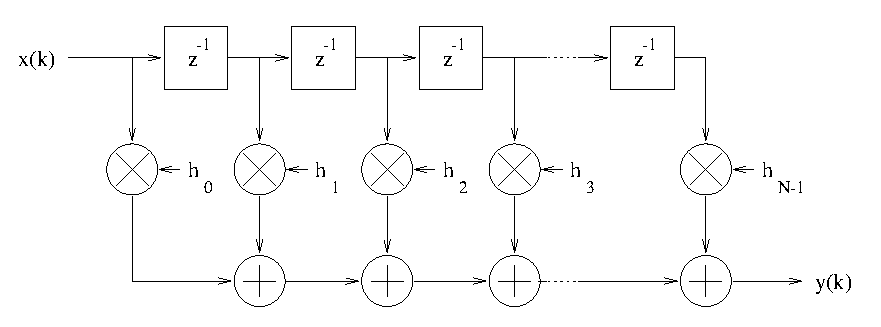
\includegraphics{fir}
  \end{center}
  \caption{\SF FIR filter block diagram.\label{FIR-filter}}
\end{figure}
%------------------ End of FIR filter -----------------------------------

One way to do this is to use a linear phase finite impulse
response (FIR) digital filter, as in figure \ref{FIR-filter}. The
input and output characteristic is defined by:
\[
      y(k) = \sum_{i=0}^{N-1} h(i) \cdot x(k-i)
\]
Linear phase is guaranteed if the filter is symmetric, i.e.:
\[
     h(k)=h(N-1-k), \mbox{ for } k=0..N-1
\]

%.........................
\subsection{Narrowband weighting}

\subsubsection{IRS weighting}

The IRS weighting corresponds to a bandpass filtering characteristic
whose mask can be found in \textcolor{blue}{Recommendation ITU-T} P.48 \cite{P.48}.
The send and receive spectral shapes of the IRS weighting were
obtained in a round-robin series of measurements made on a number of
analog telephones in the early 1970's
\cite{BNR-ModIRS}. From these measurements, the average send and
receive frequency-response characteristics were derived. However,
for the loudness balance purposes for which the IRS was designed, it
was also necessary to include a 300-3400 Hz bandpass filter, known
as the SRAEN {\em (Syst\`{e}me de R\'{e}f\'{e}rence pour la
d\'{e}termination de l'Affablissement \'{E}quivalent pour la
Nettet\'{e}; Reference System for determining Articulation Ratings)}
filter \cite{P.11, G.111}. The values of send and receive sensitivity
currently given in ITU-T Rec. P.48 (columns 2 and 3 in Table
\ref{tbl:IRS}) are therefore composed of the average send and
receive responses for a number of telephones, as well as the
response of the SRAEN filter (see column 4 of Table \ref{tbl:IRS}).

Because the P.48 IRS weighting used to be considered to model an
average narrow-band telephone handset deployed in the PSTN, the IRS
weighting has been chosen to simulate speech signals obtained from a
regular handset. Examples of standardization efforts using the P.48
weighting characteristic are the \textcolor{blue}{Recommendations
  ITU-T} G.711,
G.721, and G.728. This weighting, as defined in P.48, is sometimes
called ``full-IRS'' weighting.

While the weighting characteristic in P.48 was considered to model
connections over analog transmission facilities in the past
(although it is not clear why the SRAEN filter should be included in
both the send and receive paths), it is no longer representative of
connections over modern digital facilities. In particular, the low
frequency roll-off gives rise to unnecessary quality degradation.
For the purpose of low bit-rate coder evaluation, especially where
the coder is located in the telephone handset, a better
characteristic can be obtained by modifying the P.48 full-IRS
response to remove the SRAEN filter as shown in columns 5 and 6 of
Table \ref{tbl:IRS}. These values are specified in Annex D of
\textcolor{blue}{ITU-T Recommendation} P.830 \cite{P.830} and define the so-called
``modified'' IRS weighting. The modified IRS has been used in the
development of \textcolor{blue}{Recommendations ITU-T} G.723.1 and G.729.

\begin{table}
\Caption{14cm}{\SF \label{tbl:IRS} Send and receive amplitude
frequency
          characteristics for the IRS response as in ITU-T Rec.P.48,
          the SRAEN filter, and the modified IRS (P.48 IRS with SRAEN
          filter insertion loss removed).
        }
\begin{center}
\begin{tabular}{|c|c|c|c|c|c|}
\hline Frequency &\multicolumn{2}{|c|}{P.48 IRS}
        &SRAEN
        &\multicolumn{2}{|c|}{Modified IRS} \\
        & Send & Receive &Filter &Send & Receive \\
(Hz) & (dbPa/V) &(dbPa/V) &(dB) &(dbPa/V) &(dbPa/V) \\
\hline \hline
100     &-45.8  &-27.2  &14.1   &-31.7  &-13.4  \\
125     &-36.1  &-18.8  &11.4   &-24.7  & -7.4  \\
160     &-25.6  &-10.8  & 8.4   &-17.2  & -2.4  \\
200     &-19.2  & -2.7  & 5.9   &-13.3  &  3.2  \\
250     &-14.3  &  2.7  & 4.0   &-10.3  &  6.7  \\
300     &-11.3  &  6.4  & 2.8   & -8.5  &  9.2  \\
315     &-10.8  &  7.2  & 2.5   & -8.3  &  9.7  \\
400     & -8.4  &  9.9  & 1.4   & -7.0  & 11.3  \\
500     & -6.9  & 11.3  & 0.6   & -6.3  & 11.9  \\
600     & -6.3  & 11.8  & 0.3   & -6.0  & 12.1  \\
630     & -6.1  & 11.9  & 0.2   & -5.9  & 12.1  \\
800     & -4.9  & 12.3  & 0.0   & -4.9  & 12.3  \\
1000    & -3.7  & 12.6  & 0.0   & -3.7  & 12.6  \\
1250    & -2.3  & 12.5  & 0.0   & -2.3  & 12.5  \\
1600    & -0.6  & 13.0  & 0.1   & -0.5  & 13.1  \\
2000    &  0.3  & 13.1  &-0.2   &  0.1  & 12.9  \\
2500    &  1.8  & 13.1  &-0.5   &  1.3  & 12.6  \\
3000    &  1.5  & 12.5  & 0.5   &  2.0  & 13.0  \\
3150    &  1.8  & 12.6  & 0.3   &  2.1  & 12.9  \\
3500    & -7.3  &  3.9  & 7.0   & -0.3  & 10.9  \\
4000    &-37.2  &-31.6  &33.7   & -3.5  &  2.1  \\
5000    &-52.2  &-54.9  &43.2   & -9.0  &-11.7  \\
6300    &-73.6  &-67.5  &       & -23* &  \\
8000    &-90.0  &-90.0  &       & -40* &  \\
\hline \multicolumn{6}{|l|}{(*): Values estimated from the modified
IRS
                     implemented in the STL.}\\
\hline
\end{tabular}
\end{center}
\end{table}

\newpage
The most important part of either the full or the modified IRS
weighting is the transmission (or send) characteristic. The receive
characteristic is less important because listening is in general
done using handsets conforming to P.48 (which eliminates the need
for filtering by the software, since it is done by the telephone
terminal). In addition, the receive characteristic is relatively
flat. Some studies also show that the use of headphones instead of
handsets does not result in significantly different results while
yielding lesser listener fatigue \cite{HeadphoneACR,HeadphoneDCR}.
Nevertheless, for cases where the receive-side MIRS filter is to be
applied, a FIR implementation of this filter is available for 8000
Hz and 16000 Hz sampling rates.

An unspecified point in both P.48 and modified IRS is the phase
response of the filter. There have been discussions within UGST on
this topic and the 
conclusion was that, since the phase response is unspecified, it
should be kept as generic as possible, what is better accomplished by
keeping the phase linear\footnote{\SF In spite of that, a non-linear
phase IIR IRS filter is provided in the IIR module as an example of a
cascade-form IIR filter implementation.}. If a certain non-linear
phase characteristic is desired by the user, this can be implemented
by cascading an all-pass filter with the desired phase response with
one of the available FIR IRS implementations. Therefore, the IRS
filters are implemented as FIR filters, as depicted in Figure
\ref{FIR-filter}.

\textcolor{blue}{Recommendation ITU-T} P.48 presents the nominal values for the
amplitude response in column 2 of its Table 1 (here reproduced in
column 2 of Table \ref{tbl:IRS}) and then the upper and lower
tolerances listed in its Table 2. For the STL approach, it was decided
to design IRS filters whose characteristic would deviate no more than
0.5 dB from the average values in P.48 (see in Figure
\ref{tx-reg-irs-frq} the agreement of the nominal values, represented by
dots, and the measured frequency response for the original P.48 IRS
characteristic, represented by the continuous curve in the figure).

\subsubsection{Other weighting}

A filter that simulates the input response characteristic of certain
mobile terminals was incorporated in the STL for data sampled at 16
kHz. Figures \ref{msin-frq} and \ref{msin-ir} display the respective
frequency and impulse responses for the filter.

%% Another filter that models the input response characteristic of
%% certain super-wideband videoconferencing terminals was incorporated
%% in the STL for data sampled at 32 kHz. Figures \ref{50_14k-32k-frq}
%% and \ref{50_14k-32k-ir} show the respective frequency and impulse
%% responses for the filter.

%.........................
\subsection{Wideband weighting}
\subsubsection{P.341 weighting}

While the IRS filter is applicable to telephony bandwidth (or
narrowband) speech, for wideband speech the specification for the send
and receive sides is given in \textcolor{blue}{Recommendation ITU-T} P.341
\cite{P.341}. The mask specified in P.341 is rather wide, and an
implementation of the send-side mask agreed on by the experts has been
incorporated in the STL.

\subsubsection{Other weightings}

In the process to select a wideband codec at 32 and 24 kbit/s, a
50 Hz --5 kHz bandpass filter was developed and incorporated in the
STL. Figures \ref{bp5k-16k-frq} and \ref{bp5k-16k-ir} display the
respective frequency and impulse responses for the filter. 

A 100 Hz -- 5 kHz filter was also designed for tests of another wideband
codec. Figures \ref{bp100_5k-16k-frq} and \ref{bp100_5k-16k-ir} show
the respective frequency and impulse response of this filter.

%.........................
\subsection{Greater wideband weightings}

\subsubsection{P.341 extension weighting}
For super-wideband signals, the mask for super-wideband
videoconferencing terminals is based on the ITU-T Rec. P.341. The
sensitivity/frequency characteristics of the P.341 filter were
extended to a larger band [50 Hz - 14 kHz] with a sampling frequency
of 32 kHz.  The corresponding 50 Hz-14 kHz filter was developed and
incorporated in the STL. Figures \ref{50_14k-32k-frq} and
\ref{50_14k-32k-ir} display the respective frequency and impulse
responses for the filter.


\subsubsection{Other weightings}
To generate anchors typically used in BS.1534 \cite{BS.1534} ``MUlti
Stimulus test with Hidden Reference and Anchor (MUSHRA)'' subjective
tests, seven low-pass filters are also provided in the STL. Those
anchors are generated by low-pass filters with cut-off frequencies
1.5, 3.5, 7, 10, 12, 14 and 20~kHz at sampling frequency of
48~kHz. Their frequency responses are shown, respectively, in Figures
\ref{LP1p5-frq}, \ref{LP35-frq}, \ref{LP7-frq}, \ref{LP10-frq},
\ref{LP12-frq}, \ref{LP14-frq}, and \ref{LP20-frq}. Their impulse
responses are also given in Figures \ref{LP1p5-ir}, \ref{LP35-ir},
\ref{LP7-ir}, \ref{LP10-ir}, \ref{LP12-ir}, \ref{LP14-ir}, and
\ref{LP20-ir}. In addition a bandpass filter [20 Hz - 20 kHz)
  operating at sampling frequency of 48~kHz was also designed. Its
  frequency response is shown in figure \ref{bp20_20k-48k-frq} and its
  impulse responses in figure \ref{bp20_20k-48k-ir}.

%.........................
\subsection{Noise weighting}

Two weighting filters are available in this version of the STL,
the psophometric and the $\Delta_{SM}$ weighting filters.

The psophometric weighting curve defined by
\textcolor{blue}{Recommendation ITU-T} O.41
is used for measuring the noise level in telephone circuits,
accounting for the subjective perception of noise. The psophometric
noise measure (given in dBmp) is related to the North-American
C-message weighting curve (given in dBrnC), using to the
following:
\[
    dBmp = dBrnC - 90.0 dB
\]

The other type of signal weighting filter is the $\Delta_{SM}$, used
for converting acoustic signals recorded in the far field using an
omnidirectional microphone to the near-field equivalent of that signal
if it were in the background of a telephone user. Owing to the
directionality of the human mouth, head and torso, the high
frequencies will mainly be radiated in the frontal direction, while
the diffuse field will represent a spatial integration of the
radiation in all directions \cite{LTASS}. Hence, the $\Delta_{SM}$
filter is deployed for weighting acoustic noises (babble, vehicular,
etc.) before electrical summation with clean speech files, in order to
simulate speech corrupted by background noise. It is useful in
subjective listening tests where precise control of the actual SNR is
necessary.

Both these filters have been implemented as FIR filters. The
psophometric filter has been designed for speech sampled at 8 kHz, and
the $\Delta_{SM}$ filter for speech sampled at 16 kHz. It should be
noted that these filters, like the IRS filters, are also
frequency-specific and, unlike the low-pass high-quality FIR filters
described before, cannot be used for arbitrary rate ratio conversion.

%........................
\subsection{PCM Quality}

There are applications requiring the simulation of the response of
filters found in the A/D and D/A interfaces of current transmission
systems, which are in general PCM systems satisfying
\textcolor{blue}{Recommendation ITU-T} 
G.711. The filters associated with G.711 are specified in Recommendation
\textcolor{blue}{ITU-T} G.712 \cite{G.712}. The main characteristic of these filters is the
low out-of-band rejection of 25 dB.

%------------------ Begin of parallel-form IIR filter --------------------
\begin{figure}[h]
  \begin{center}
    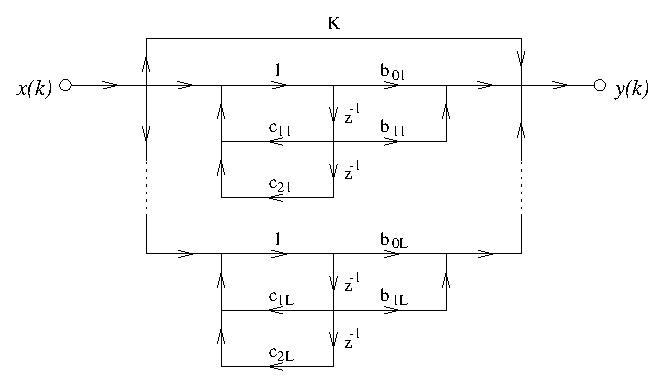
\includegraphics{iir-par}
  \end{center}
  \caption{\SF Parallel-form IIR filter block diagram.\label{IIR-filter}}
\end{figure}
%------------------ End of IIR filter -----------------------------------

In this context it is also necessary to simulate the convertion back
to and forth the analog domain, e.g. to simulate multiple transcodings
which are called {\em asynchronous trancodings}\footnote{\SF As the
name indicates, there is no synchronization between sampling instants
of the two digital systems, i.e., re-sampling in the succeeding A/D is
not synchronous to the clock in the preceding D/A converter.}. One
way to simulate asynchronous transcodings is by means of a non-linear
phase filter (non-constant group delay), which is most efficiently
implemented using IIR filters.

Infinite impulse response (IIR) filters used in this tool are of the
parallel form (see figure \ref{IIR-filter}), described by the
equation:
\[
    H_I^p(z) = K + \sum_{l=1}^{L}
                    { b_{0l}+b_{1l} z^{-1} \over
                      \ 1+c_{1l} z^{-1}+ c_{2l} z^{-2} \
                    }
\]
and of the cascade form (see figure \ref{IIR-cascade-filter}), described
by the equation:
\[
    H_I^c(z) = \prod_{l=1}^{N}
                    { b_{0l} + b_{1l} z^{-1} + b_{2l} z^{-2}\over
                           1 + c_{1l} z^{-1} + c_{2l} z^{-2}
                    }
\]

%------------------ Begin of cascade-form IIR filter --------------------
\begin{figure}
  \begin{center}
    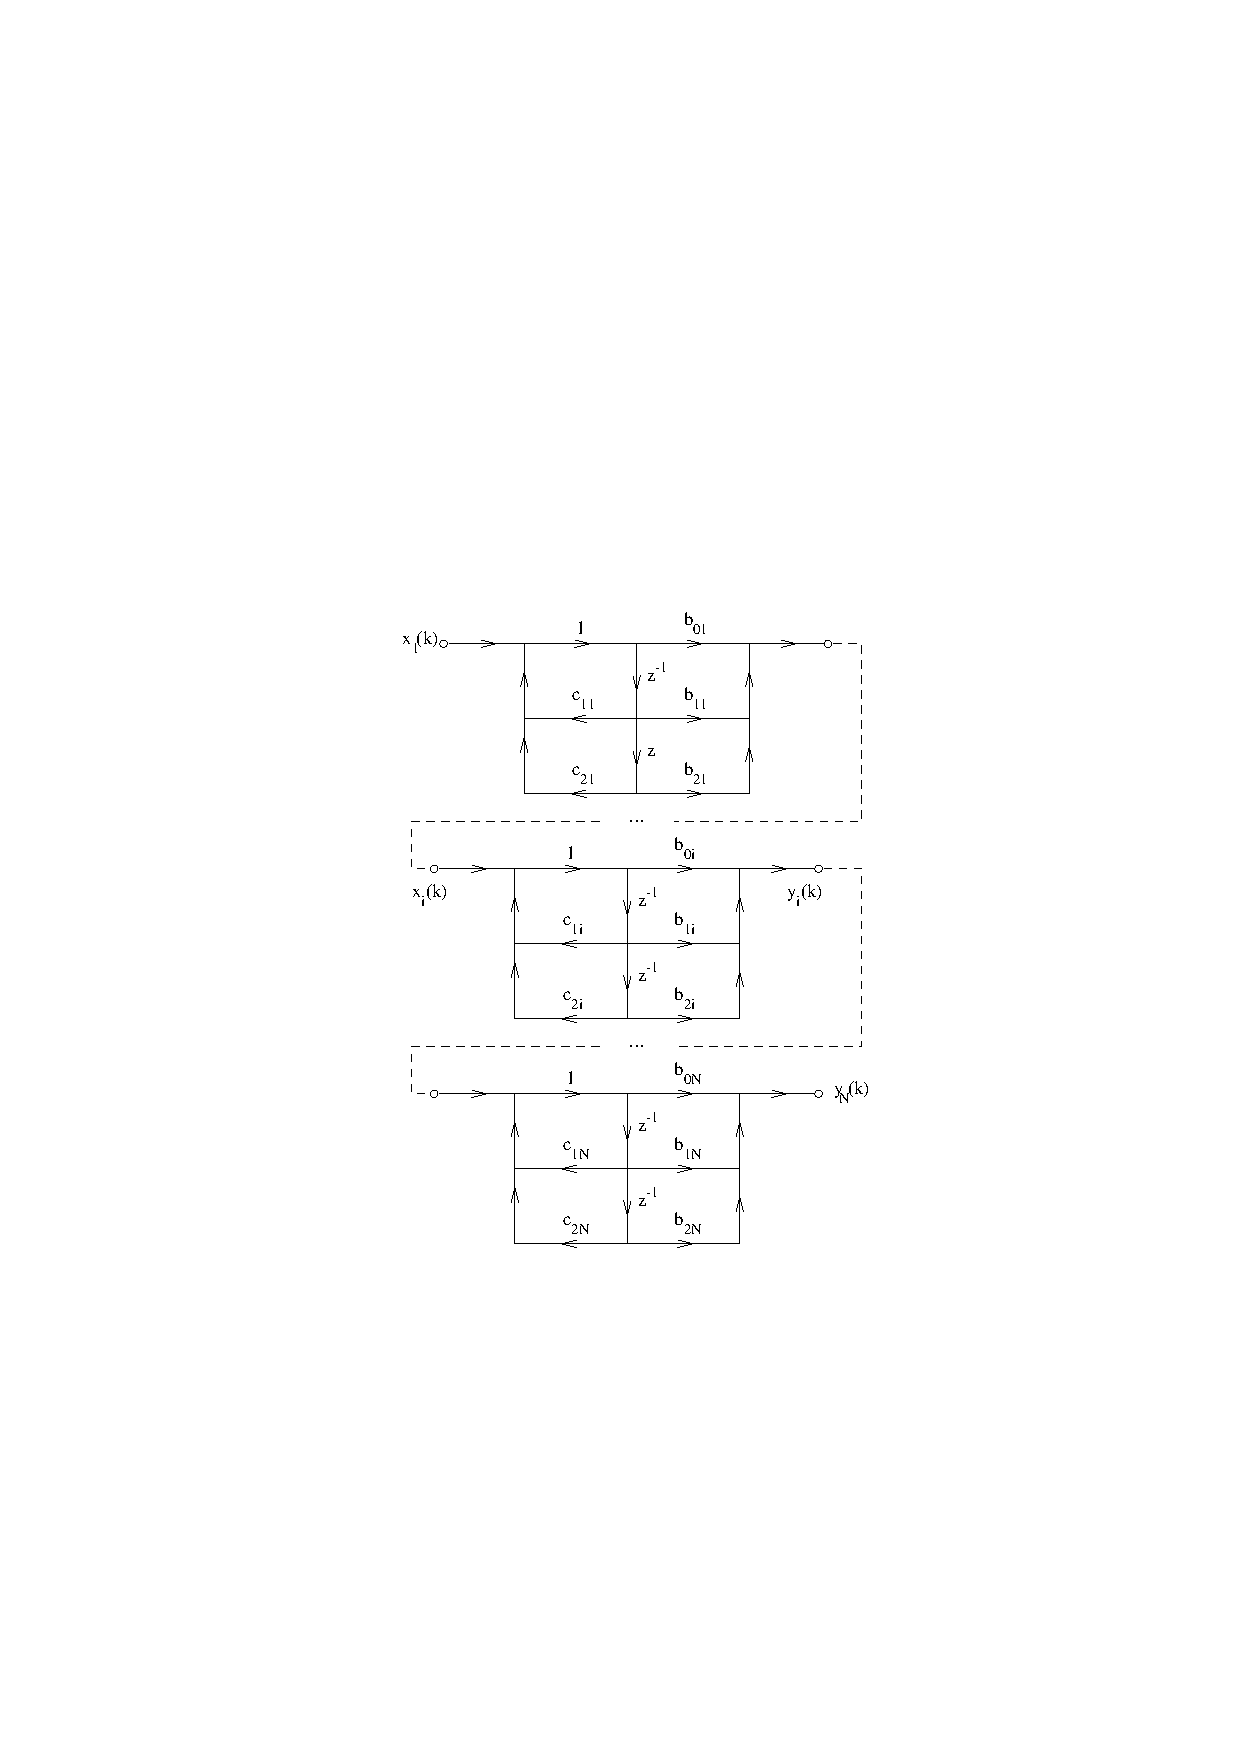
\includegraphics{iir-casc}
  \end{center}
  \caption{\SF Cascade-form IIR filter block diagram.
               \label{IIR-cascade-filter}}
\end{figure}
%------------------ End of IIR filter -----------------------------------


%=============================
\section{Implementation}

The rate change algorithm is organized in two modules, FIR and IIR,
with prototypes respectively in {\tt firflt.h} and {\tt iirflt.h}. It
evolved from a version initially developed as part of the ETSI
Half-rate GSM codec Host Laboratory exercise \cite{SCD-ETSI}. The
rate-change functionality was incorporated in the STL92 in two main
files, {\tt hqflt.c} and {\tt pcmflt.c}.  To make these routines more
flexible, the following modifications were included:
\begin{itemize}
 \item[FIR:] the FIR module was divided into a library source file ({\tt
        fir-lib.c}) containing the basic filtering and
        initialization functions, as well as into source files for each kind of
        filter: {\tt fir-flat.c} for high-quality low-pass and bandpass
        filters, {\tt fir-irs.c} for the classical and modified IRS
        filters, and so on;
 \item[IIR:] the IIR module was divided into a library file ({\tt
        iir-lib.c}) containing basic filtering and
        initialization functions, as well as into source files for each kind of
        filter: {\tt iir-g712.c} for G.712 filtering using the
        parallel-form filters, {\tt iir-flat.c} for flat bandpass 1:3
        and 3:1 asynchronization filtering using a cascade-form
        filter, and so on.
\end{itemize}

Files {\tt fir-*.c} of the FIR module contain all the routines
implementing FIR filters, i.e., the high-quality filters and IRS,
$\Delta_{SM}$ and psophometric weighing filters. Files {\tt iir-*.c}
of the IIR module implement the IIR filters, i.e., the parallel-form PCM
filter and the cascade-form 3:1 asynchronization filter.

Some of these filters have been implemented using 24-bit coefficients,
thus allowing real-time, bit-exact hardware implementation of these
routines. It may be noted that, for these filters in the STL, the
calculations are performed in floating-point arithmetics by converting
the coefficients from the range $\SF -2^{23}$..$\SF 2^{23}$--1 to $-1
.. +1$, which is not needed in real time hardware with fixed-point
DSPs.

Frequency response and impulse response plots are provided for the
STL filters in the forthcoming sections. It should be noted,
however, that the impulse responses shown have been computed from
the 16-bit quantized impulse responses of the filters, as generated
by the demonstration programs, while the frequency responses were
calculated as described in section \ref{RATE-Tests}. It should be
noted that the apparent asymmetry in some impulse responses happens
because an integer number of samples are generated, and linear
interpolation is used to draw the figure. If the impulse responses
were derived directly from the filter coefficients, the plot would
be symmetric.


\NOTE{158mm}{
                When the same filter type is used by several
                independent speech materials (e.g. several speech
                files) within the same execution of an application
                program, the user must remember that the filters have
                memory. Hence, wrong results can be obtained if a
                given number of initial samples are not discarded.
                See section \ref{Rate-exp} for an example, where the
                first 512 samples are skipped when calculating the
                power level of the output tone.
}


%-.-.-.-.-.-.-.-.-.-.-.-.-.-.-.-.-
\subsection{FIR module}

The frequency responses of the implemented high-quality low-pass
filters are shown in figures \ref{hq-frq-1-2} and \ref{hq-frq-1-3}
(for rate-change factors 2 and 3, respectively), while the telephone
bandwidth bandpass filter is given in figure \ref{hq-bandpass} (only
a rate-change factor of 2 is available). The impulse responses of
these filters are given in figures \ref{ir-hq-up}, \ref{ir-hq-down},
and \ref{ir-bandpass}, respectively for the up-sampling filters
(factors 2 and 3), for the down-sampling filters (factors 2 and 3),
and for the bandpass filter.

The transmit-side IRS filter has been implemented for the ``regular''
and modified flavors. The regular transmit-side P.48 IRS filter
amplitude responses are shown in figure \ref{tx-reg-irs-frq} (the
available sampling rates are 8 and 16 kHz). The transmit-side modified
IRS filter is available for sampling at 16 kHz and 48 kHz, and
their frequency responses are shown in figure \ref{tx-mod-irs-frq}.
The impulse response of these transmit-side IRS filters are in figures
\ref{tx-reg-irs-ir} and \ref{tx-mod-irs-ir} for the regular and
modified IRS filters, respectively. The receive-side modified IRS
filter has also been implemented and the frequency responses for 8 kHz
and 16 kHz sampling rate are found in figure \ref{rx-mod-irs-frq}. The
impulse responses of the receive-side modified IRS filters are shown in
figure \ref{rx-mod-irs-ir}.

The frequency response of the STL psophometric filter is given in
figure \ref{pso-08k-frq}, and that of the $\Delta_{SM}$ filter in figure
\ref{delta-sm-frq}.

For wideband signals, three weighting filters are available. The
transmit-side ITU-T P.341 filter amplitude response is shown in
figure \ref{tx-p341-frq}, and its impulse response is shown in
figure \ref{tx-p341-ir}. Alternatively to the P.341 filter, the
frequency and impulse responses of the two bandpass filters,
50 Hz-5 kHz bandpass filter and 100 Hz -5 kHz, are shown, respectively,
in figures \ref{bp5k-16k-frq} and \ref{bp5k-16k-ir}, and in figures
\ref{bp100_5k-16k-frq} and \ref{bp100_5k-16k-ir}.

For super wideband signals, four weighting filters are available.
The 50 Hz-14 kHz bandpass filter, extension of ITU-T P.341 filter, is
presented in figures \ref{50_14k-32k-frq} (frequency response), and
\ref{50_14k-32k-ir} (impulse response). Alternatively to this P.341
filter extension, the frequency responses of the three MUSHRA
anchors filters, LP3.5, LP7 and LP10 filters, are shown in figures
\ref{LP35-frq}, \ref{LP7-frq} and \ref{LP10-frq}, respectively.
Their impulse responses are shown in figures \ref{LP35-ir},
\ref{LP7-ir} and \ref{LP10-ir}, respectively.

The high-quality filters were implemented for rate-change factors
of 2 and 3. The IRS filters, band-limiting filters and MUSHRA
anchors have been designed for specific {\em sampling rates} (e.g.
8 and 48 kHz). It should be noted that, while the high-quality
filters are independent of the rate, these filters are not,
because their masks are specified in terms of Hz, rather than
normalized frequencies. This means that to carry out a
high-quality up-sampling from 8 to 16 kHz, and from 16 to 32 kHz,
the same routines are called, while for IRS, band-limiting or
MUSHRA anchors, there is no rate-change routine from 16 to 32 kHz.

Since the digital filters have memory, state variables are needed. In
this version of the STL, a type {\tt SCD\_FIR} is defined, containing the past
sample memory, as well as filter coefficients and other control
variables. Its fields, whose values shall never be changed by the
user, are as follows:
\begin{quote} \normalsize
 {\em lenh0}    \dotfill \parbox{110mm}{\SF Number of FIR coefficients}\\
 {\em dwn\_up}  \dotfill \ \parbox{110mm}{\SF Down-sampling factor }\\
 {\em k0}       \dotfill \parbox[t]{110mm}{\SF Start index in next segment
                                       (needed in segment-wise filtering) }\\
 {\em h0}       \dotfill \parbox{110mm}{\SF Pointer to array with FIR
                                          coefficients }\\
 {\em T}        \dotfill \parbox{110mm}{\SF Pointer to delay line }\\
 {\em hswitch}  \dotfill \parbox{110mm}{\SF Switch to FIR-kernel: up- or down-
                                          sampling }\\
\end{quote}

The relevant routines for each module are described in the next
sections.\footnote{\SF It should be noted that in the source code
files there are local (privately-defined) functions which are not
intended to be directly accessed by the user and therefore are not
described here.}


%----------- Begin of FIR filters response : frq for factor 2 ---------------
\begin{figure}[hbtp]
  \begin{center}
    %Both boxes' dimension: 15.24cm x  8.89cm
        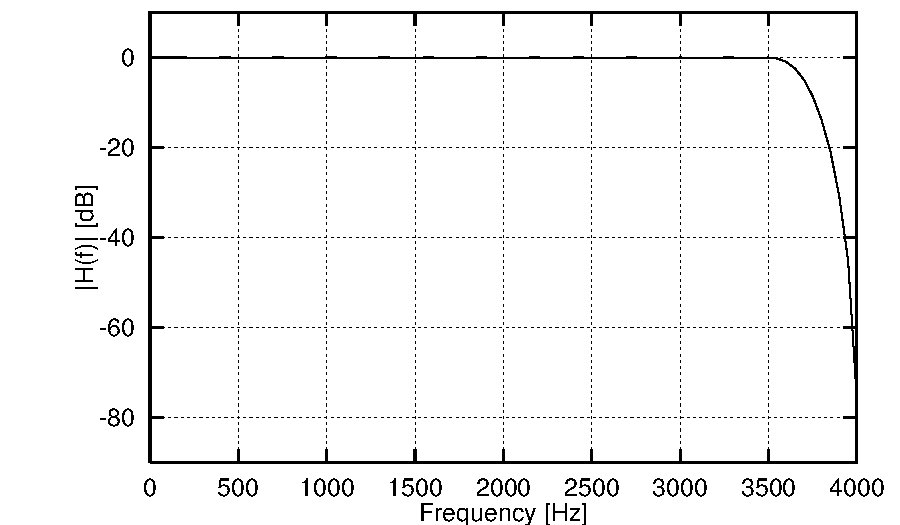
\includegraphics{hq2_1_2}
    \\
   (a) High-quality filter for up-sampling.

        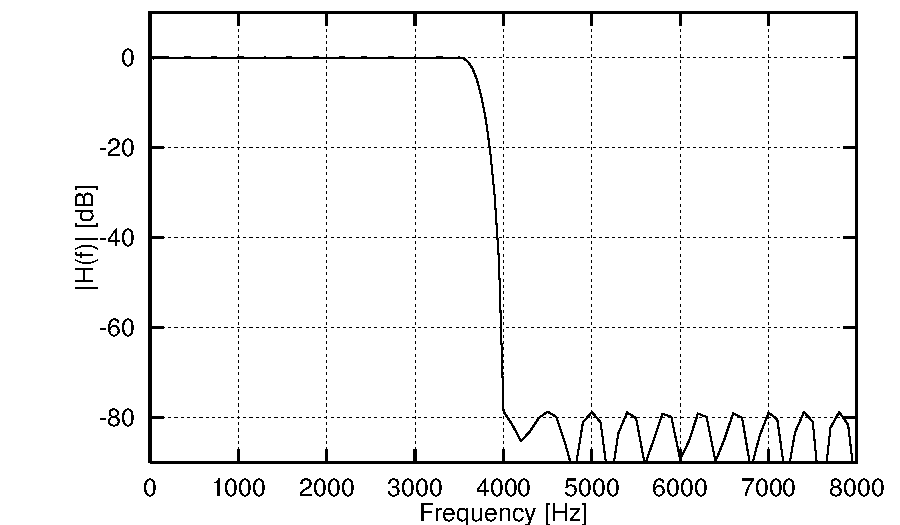
\includegraphics{hq2_2_1}
    \\
   (b) High-quality filter for down-sampling.

  \end{center}
  \caption{\SF High-quality filter responses for a
               factor of 2 and sampling rates of 8000 and
               16000 Hz.\label{hq-frq-1-2}}

\end{figure}
%------------- End of FIR filters response: frq for factor 2 ----------------

%----------- Begin of FIR filters response: frq for factor 3 ---------------
\begin{figure}[hbtp]
  \begin{center}
    %Both boxes' dimension: 15.24cm x  8.89cm
        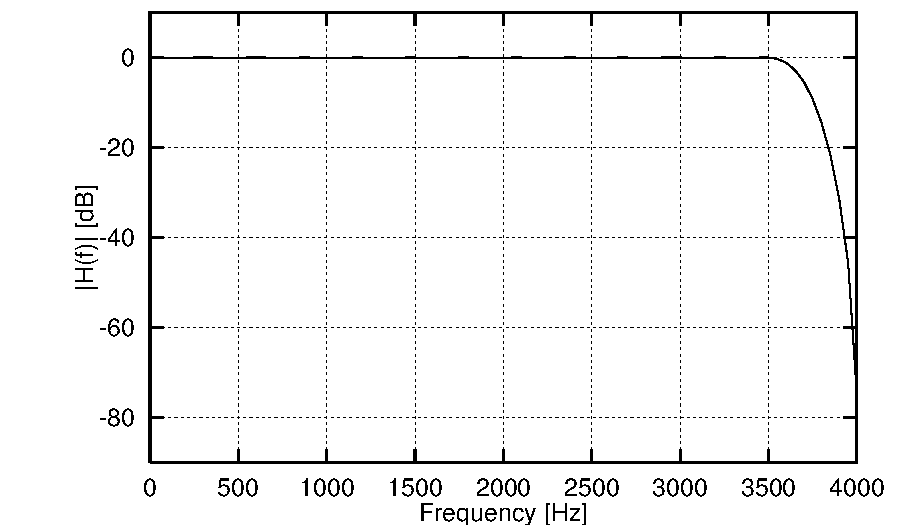
\includegraphics{hq3_1_3}
    \\
   (a) High-quality filter for up-sampling.

        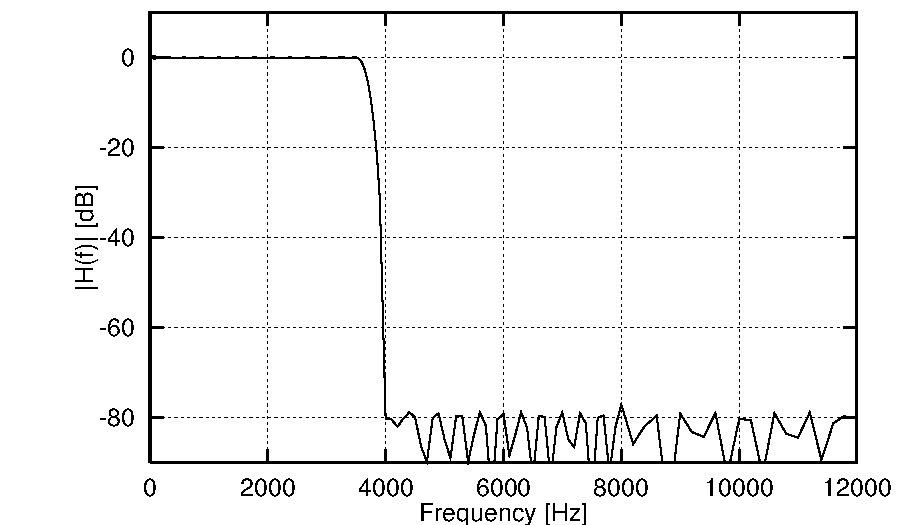
\includegraphics{hq3_3_1}
   \\
   (b) High-quality filter for down-sampling.

  \end{center}
  \caption{\SF High-quality filter responses for a
               factor of 3 and sampling rates of 8000 and
               24000 Hz.\label{hq-frq-1-3}}

\end{figure}
%------------- End of FIR filters response: frq for factor 3 ----------------


%----------- Begin of FIR filters response: frq for bandpass filter  --------
\begin{figure}[hbtp]
  \begin{center}
 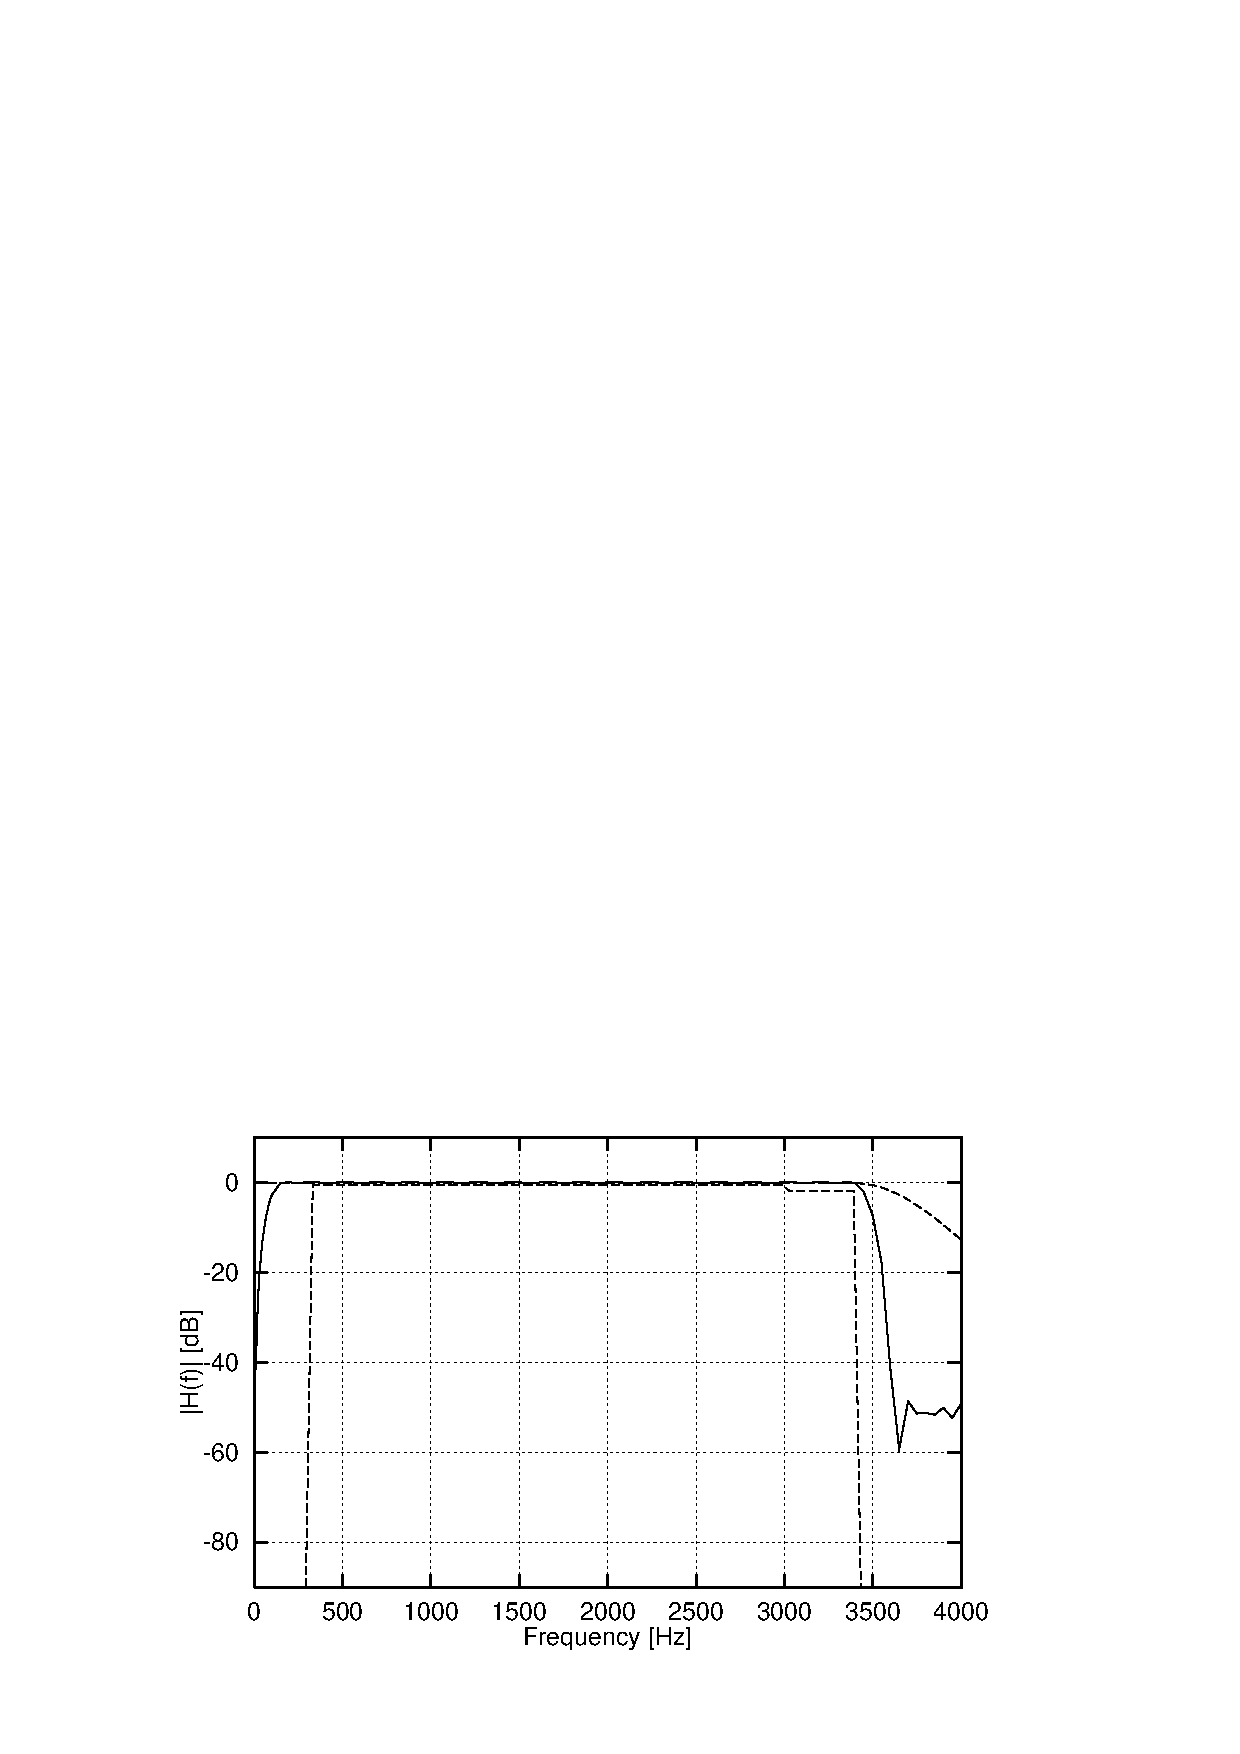
\includegraphics{flat_1_2}
 \\
   (a) High-quality bandpass for up-sampling (factor 1:2).

 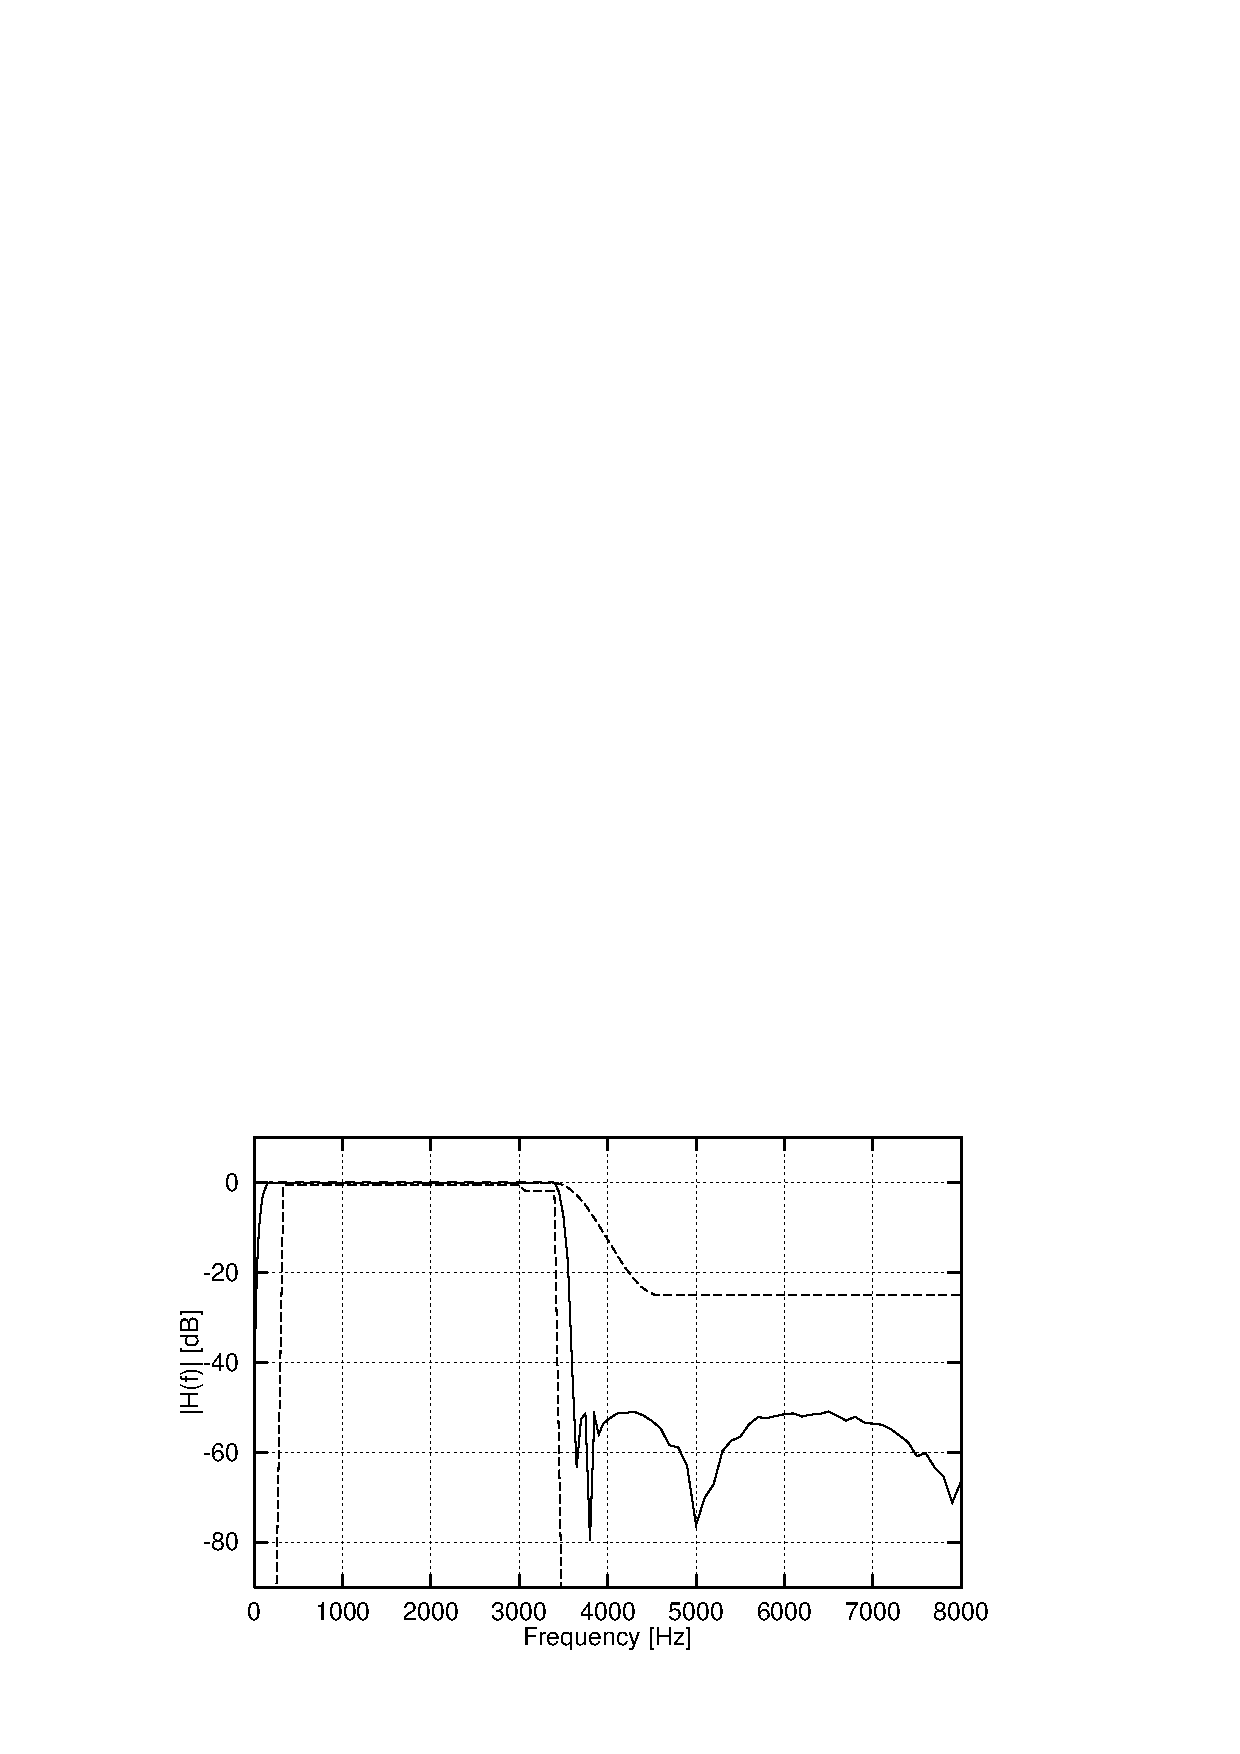
\includegraphics{flat_2_1}
 \\
   (b) High-quality bandpass for 2:1 down-sampling or for 1:1
       filtering.

  \end{center}
  \caption{\SF High-quality bandpass filter responses. Mask shown is
           that of the G.712 filter, for reference.
           \label{hq-bandpass}
          }
\end{figure}
%------------- End of FIR filters response: frq for bandpass ----------------


%--- Begin of FIR filters response: impulse response for UP filters ------
%Box dimension: 16.05cm x 18.03cm
\begin{figure}[hbtp]
  \begin{center}
 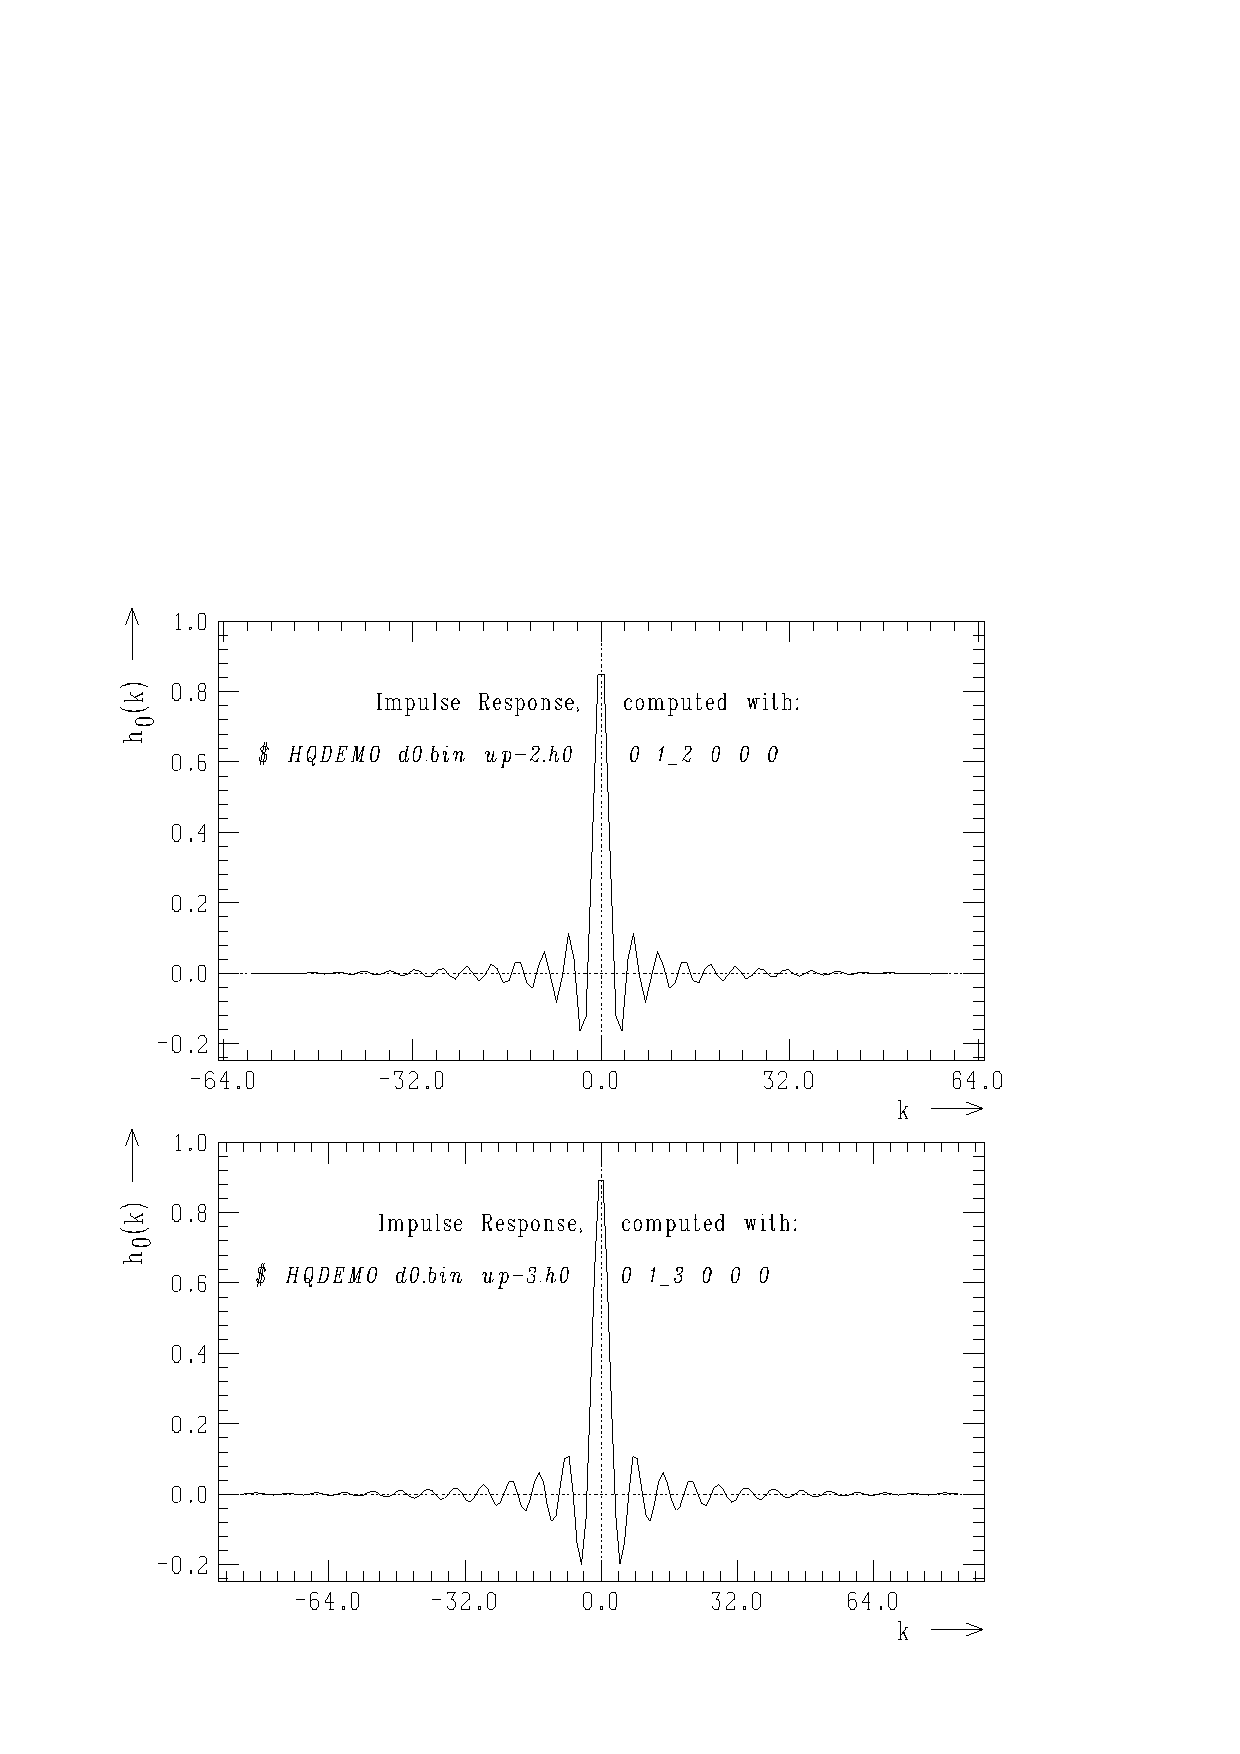
\includegraphics{hqup-h0}
  \end{center}
  \caption{\SF Impulse response for high-quality
               up-sampling filters (top, factor of 2; bottom,
               factor of 3).\label{ir-hq-up}}
\end{figure}
%----- End of FIR filters response: impulse response for UP filters ------


%--- Begin of FIR filters response: impulse response for DOWN filters ------
%Box dimension: 16.05cm x 18.03cm
\begin{figure}[hbtp]
  \begin{center}
 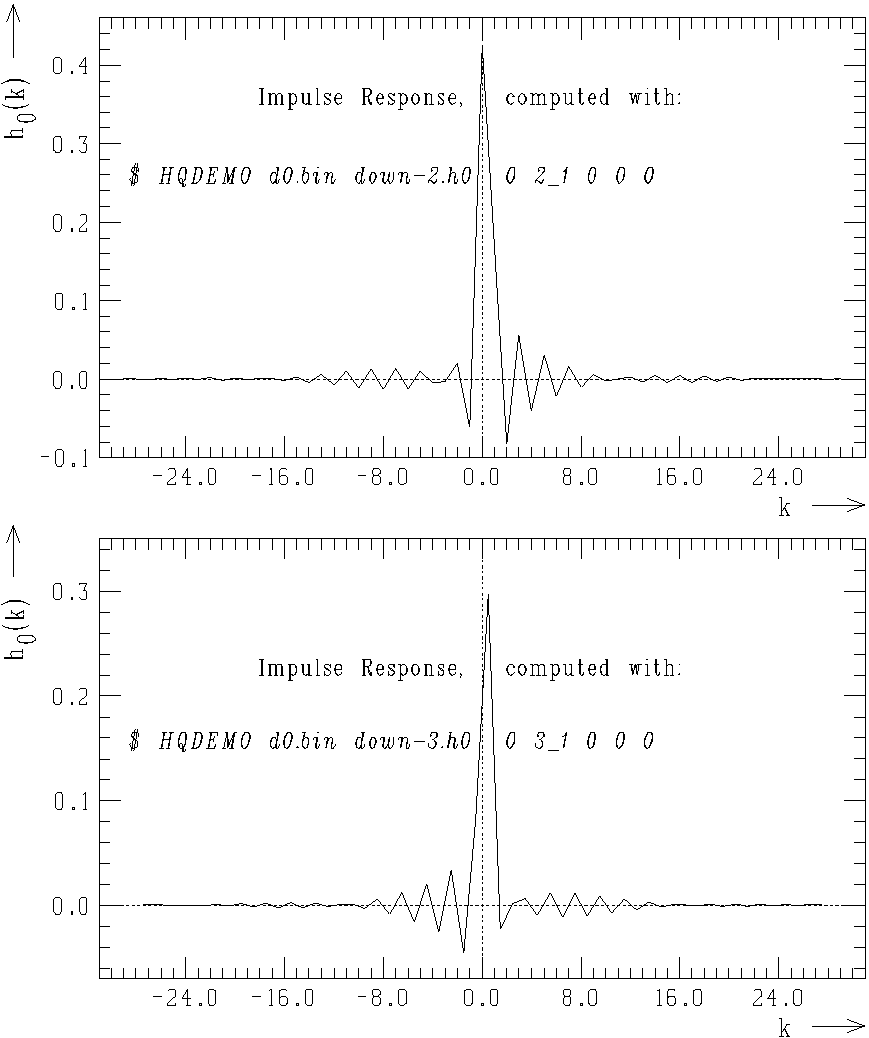
\includegraphics{hqdw-h0}
  \end{center}
  \caption{\SF Impulse response for high-quality
               down-sampling filters (top, factor of 2;
               bottom, factor of 3).\label{ir-hq-down}}
\end{figure}
%----- End of FIR filters response: impulse response for DOWN filters ------


%--- Begin of FIR filters response: impulse response for bandpass filter ----
%Box dimension: 16.05cm x 18.03cm
\begin{figure}[hbtp]
  \begin{center}
 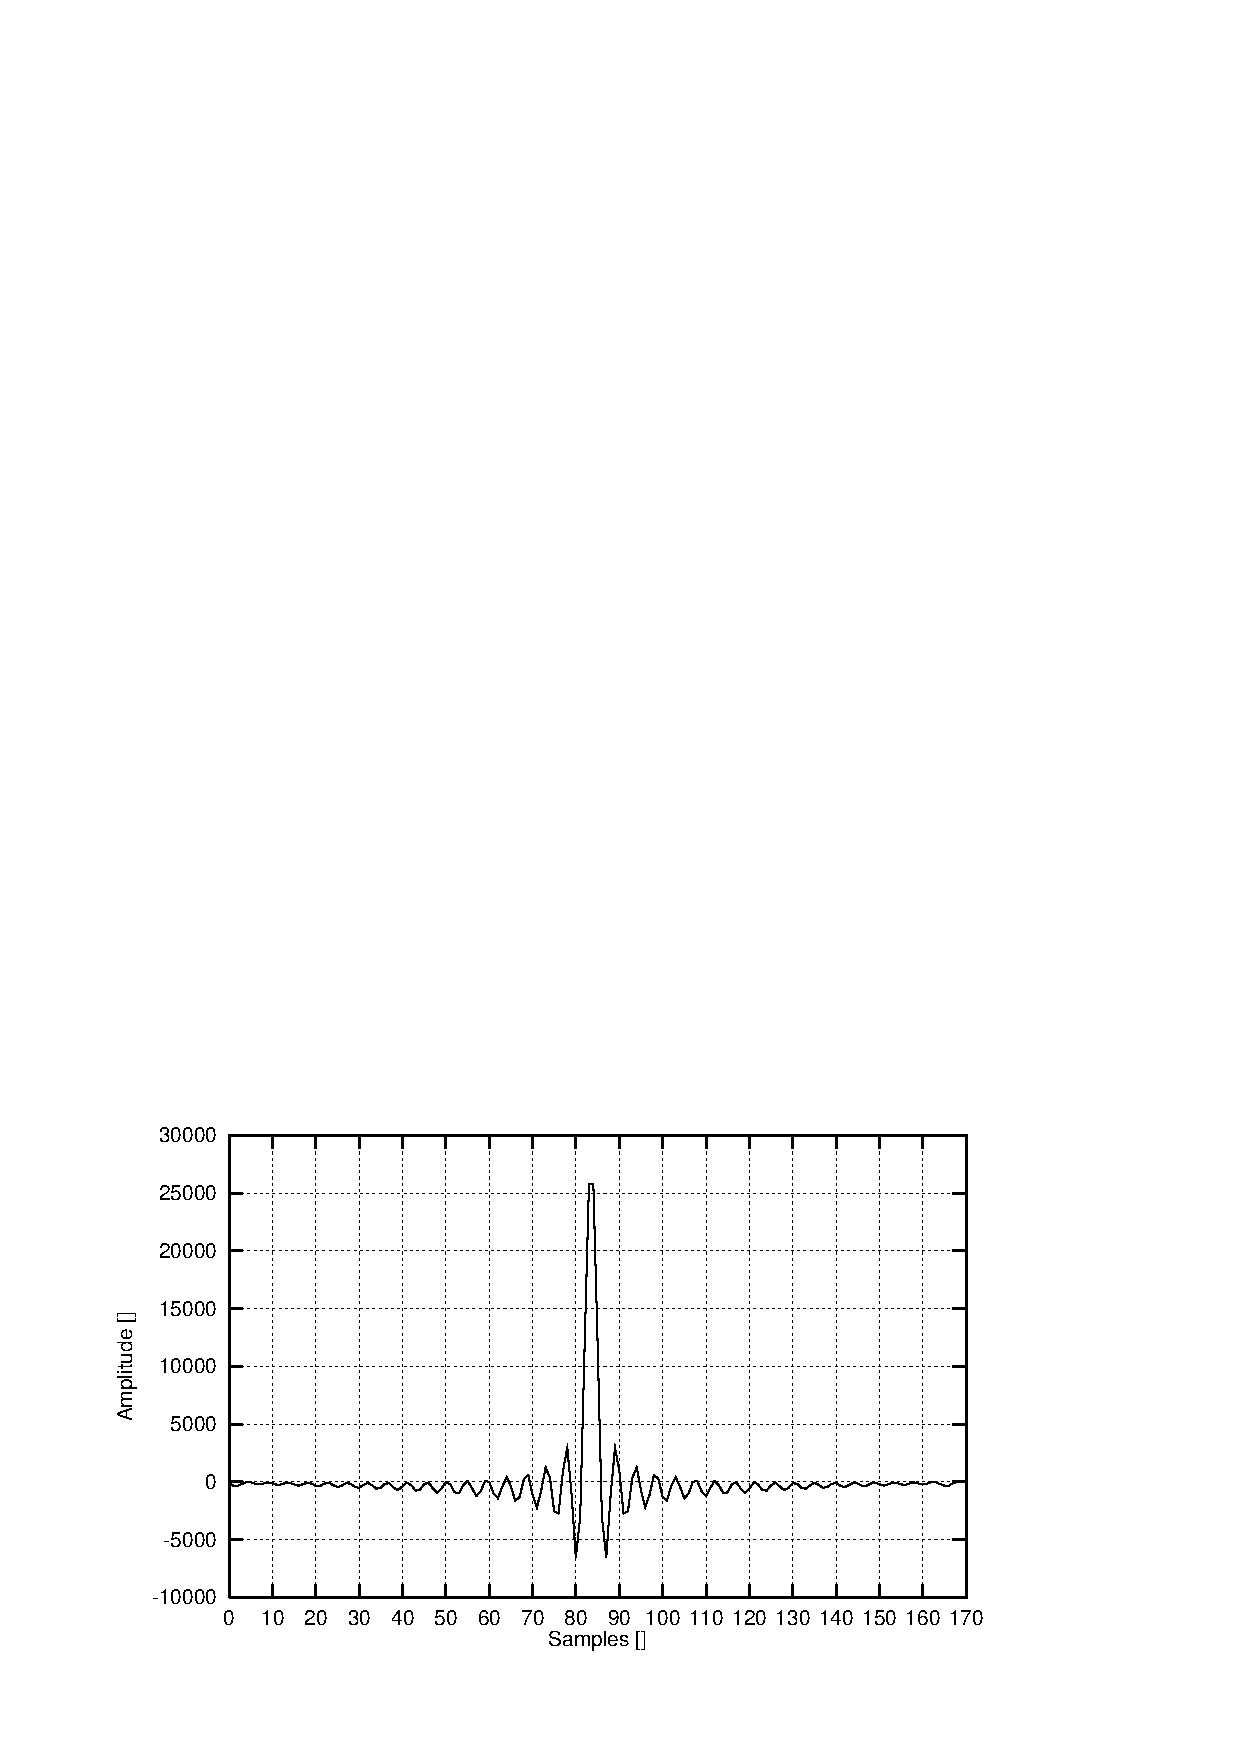
\includegraphics{bpup-h0}
 \\
   (a) High-quality bandpass for up-sampling (factor 1:2).

 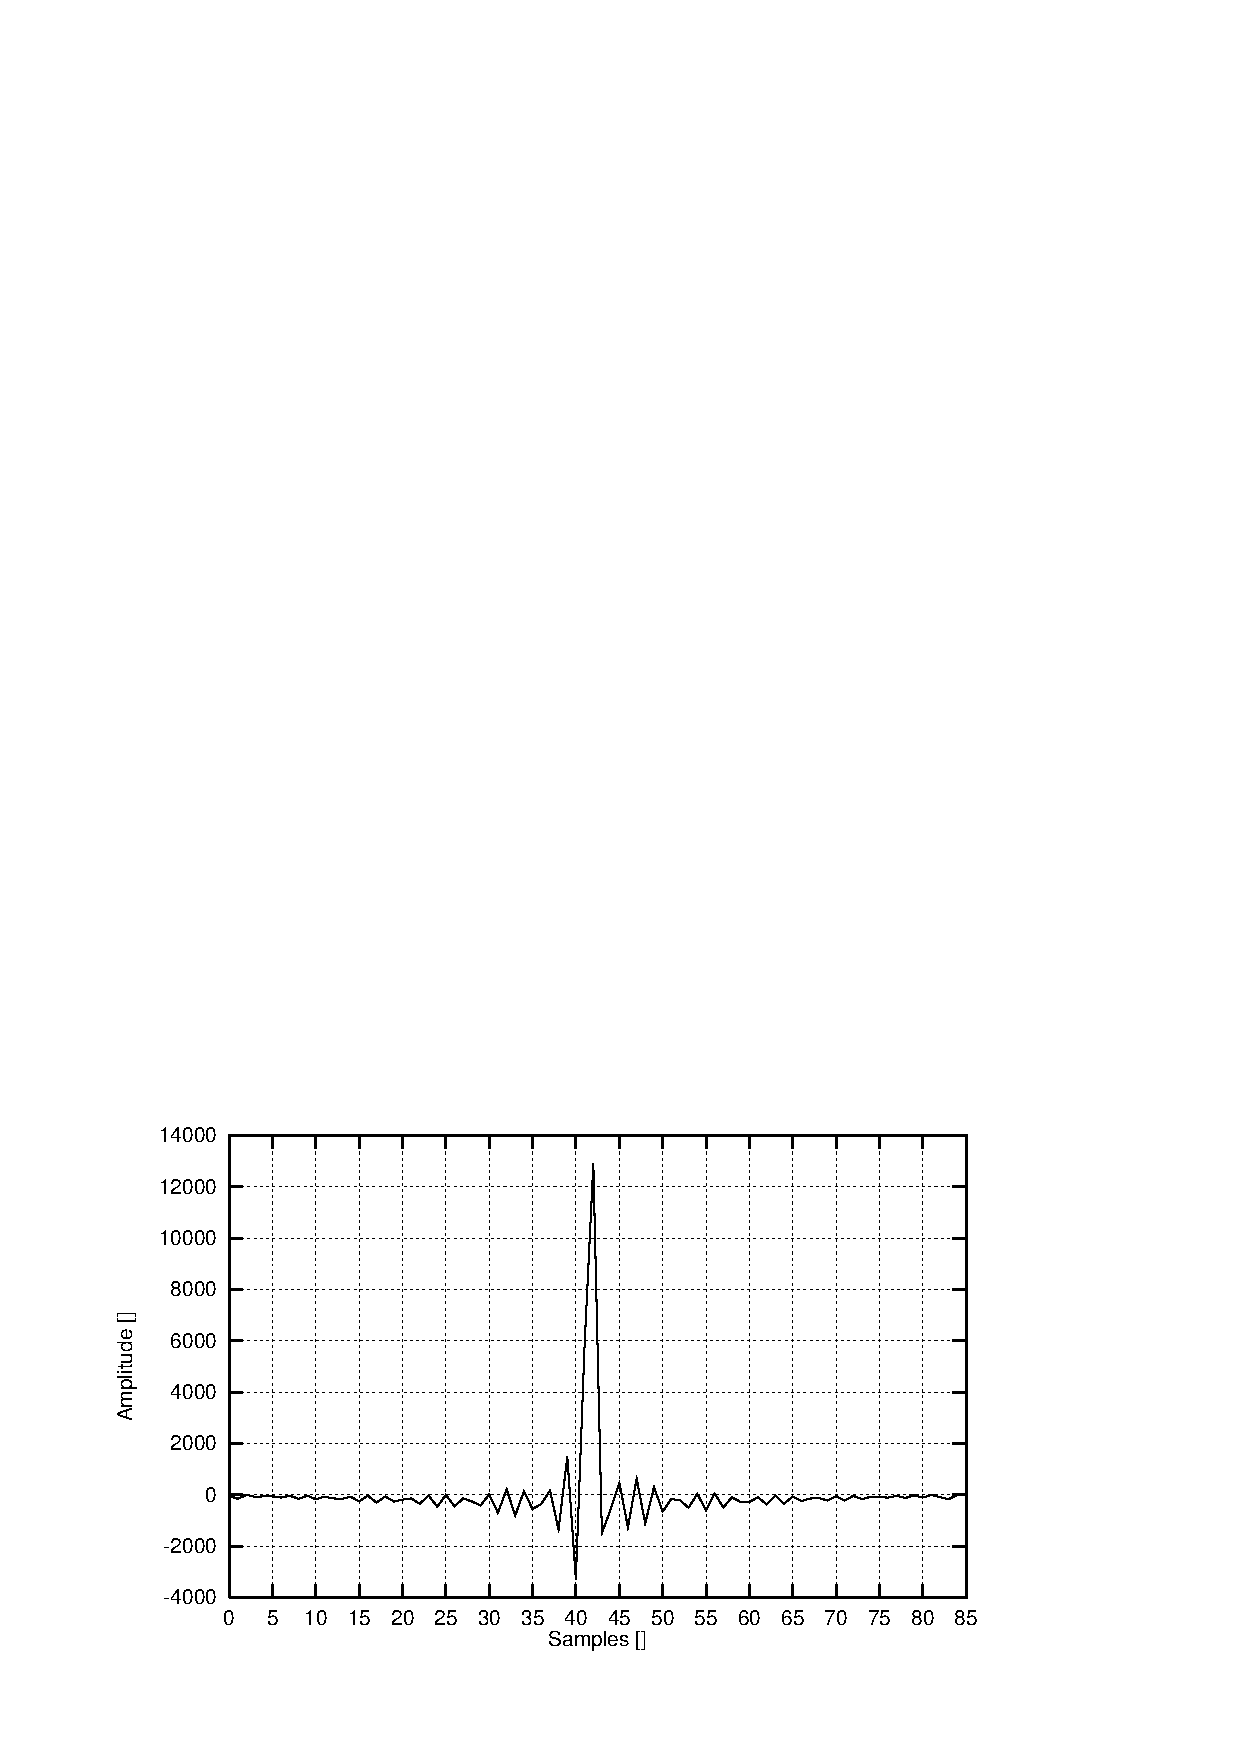
\includegraphics{bpdw-h0}
 \\
   (b) High-quality bandpass for down-sampling (factor 2:1).

  \end{center}
  \caption{\SF Impulse response for high-quality
               bandpass filter (factors 2:1 and 1:1). Top is
               up-sampling by a factor of 1:2, and bottom is
               down-sampling by a factor of 2:1. \label{ir-bandpass}}
\end{figure}
%----- End of FIR filters response: impulse response for bandpass filter ---


%----------- Begin of FIR filters response: frq for MSIN filter  --------
\begin{figure}[hbtp]
  \begin{center}
 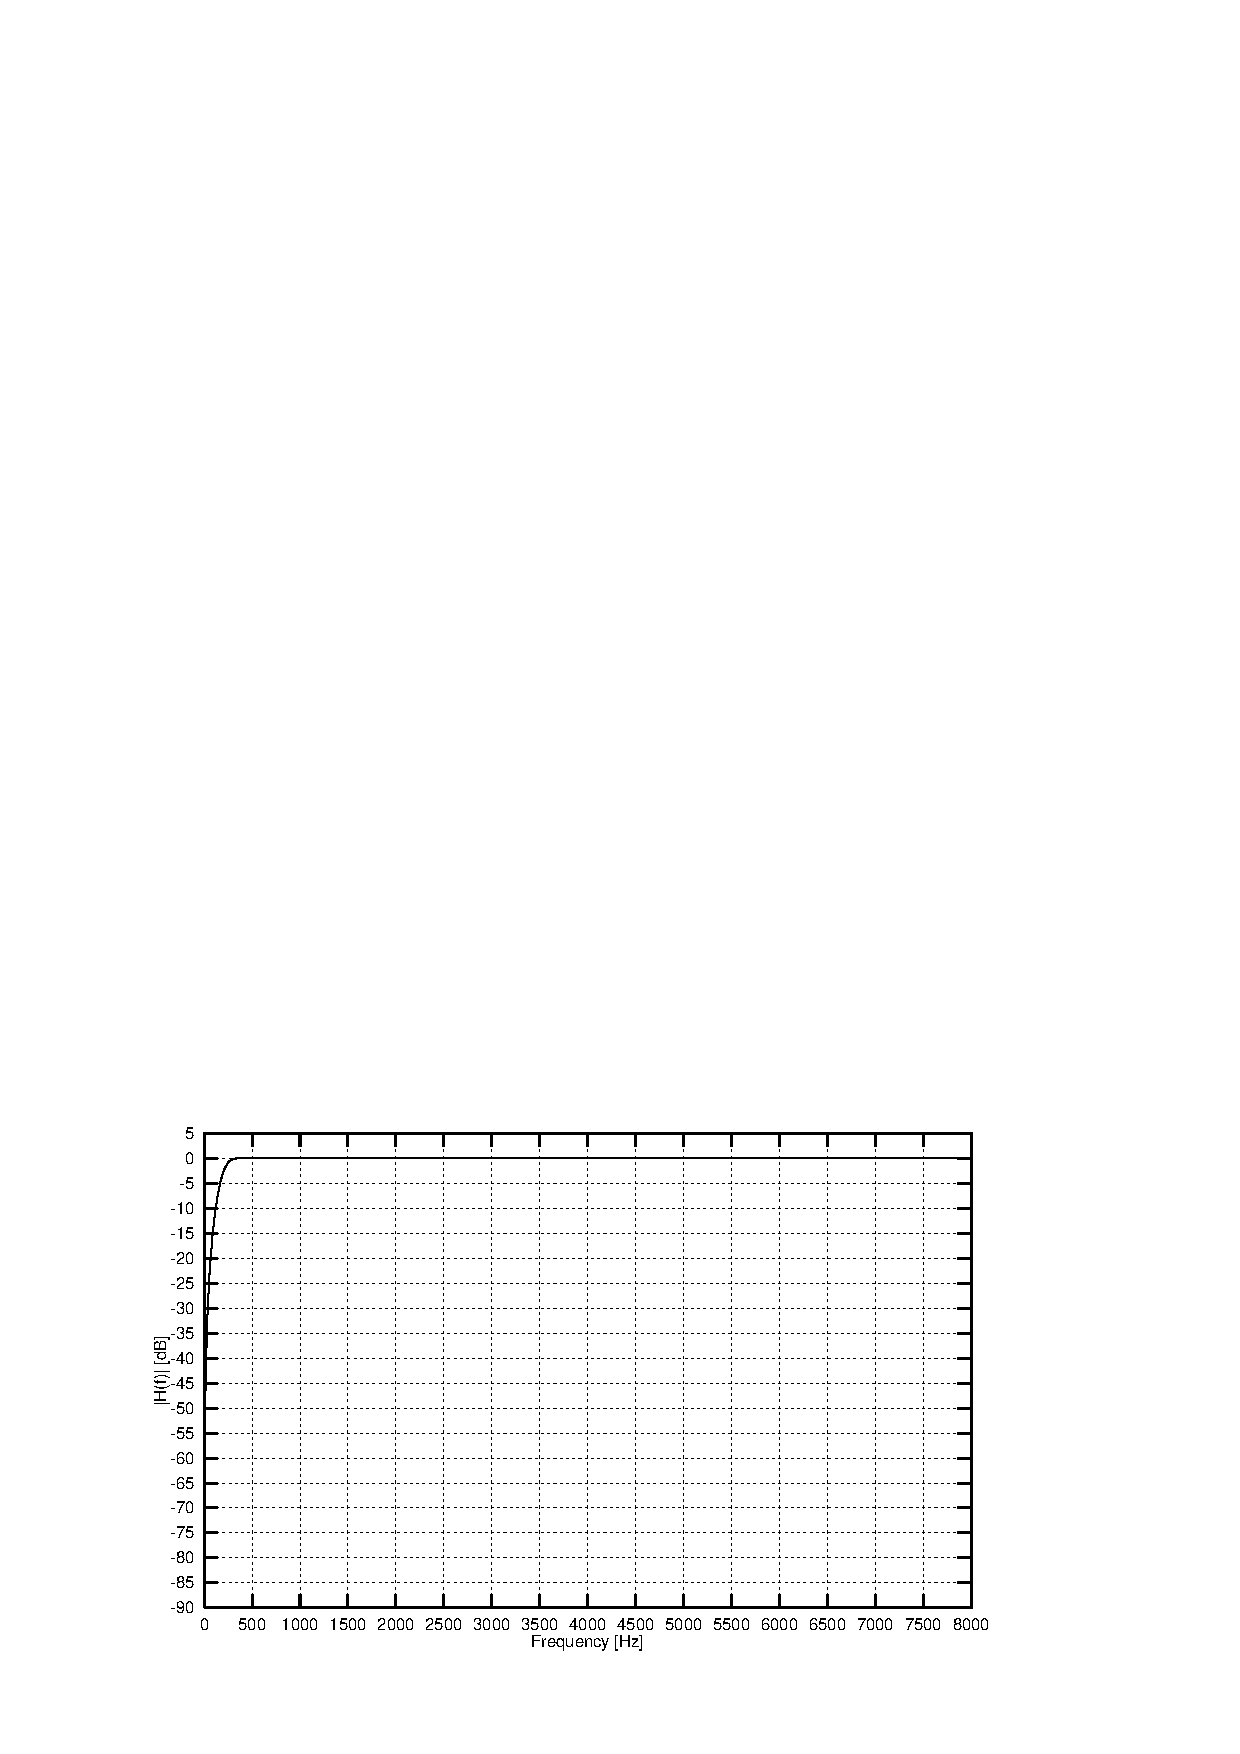
\includegraphics{msin16}
  \end{center}
  \caption{\SF STL mobile station input (MSIN) frequency response for data
               sampled at 16 kHz (factor 1:1).
           \label{msin-frq}
          }
\end{figure}
%------------- End of FIR filters response: frq for MSIN ----------------


%--- Begin of FIR filters response: impulse response for MSIN --------
\begin{figure}[hbtp]
  \begin{center}
 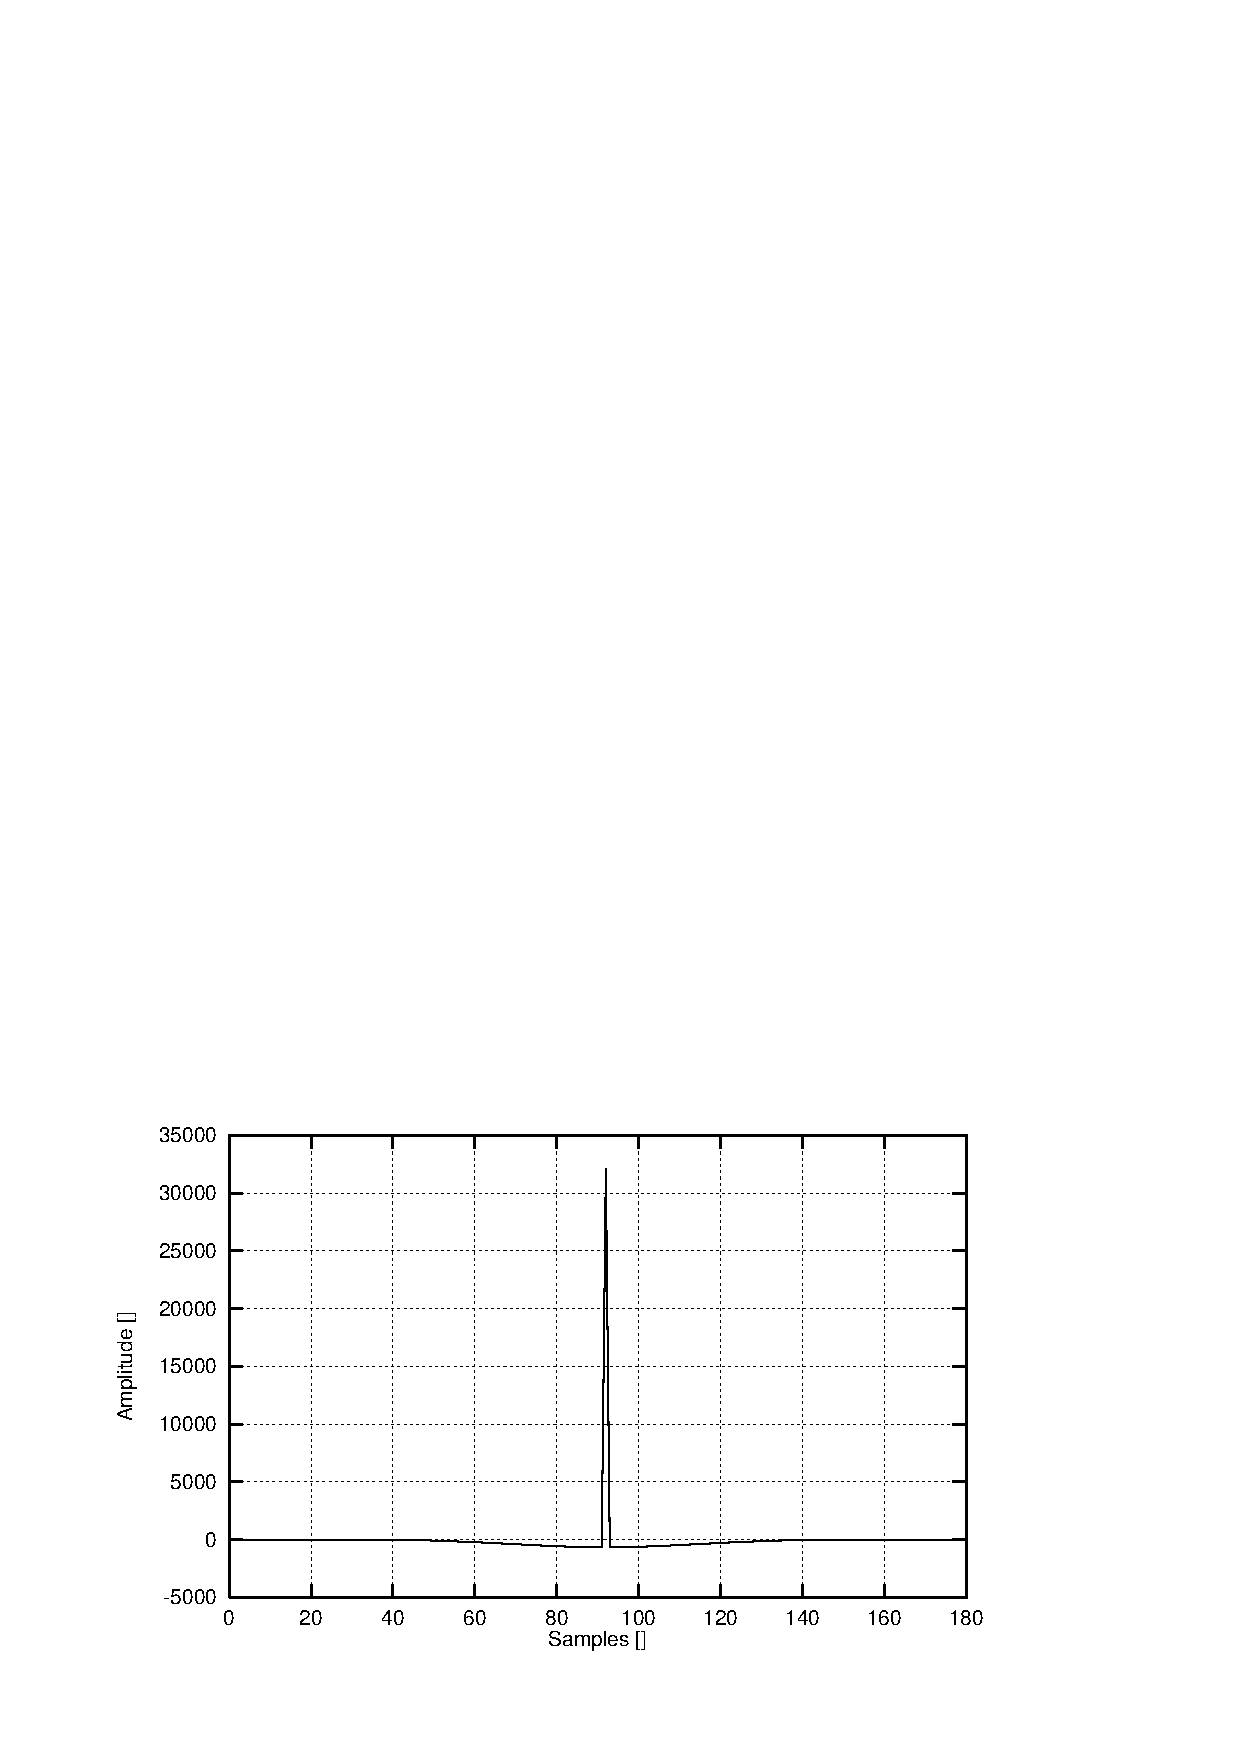
\includegraphics{msin16-h0}
  \end{center}
  \caption{\SF STL MSIN send-side filter impulse response.
           \label{msin-ir}
          }
\end{figure}
%----- End of FIR filters response: impulse response for MSIN -----

\flushfloats

%------------------ Begin of regular IRS filters response --------------------
\begin{figure}[hbtp]
  \begin{center}
 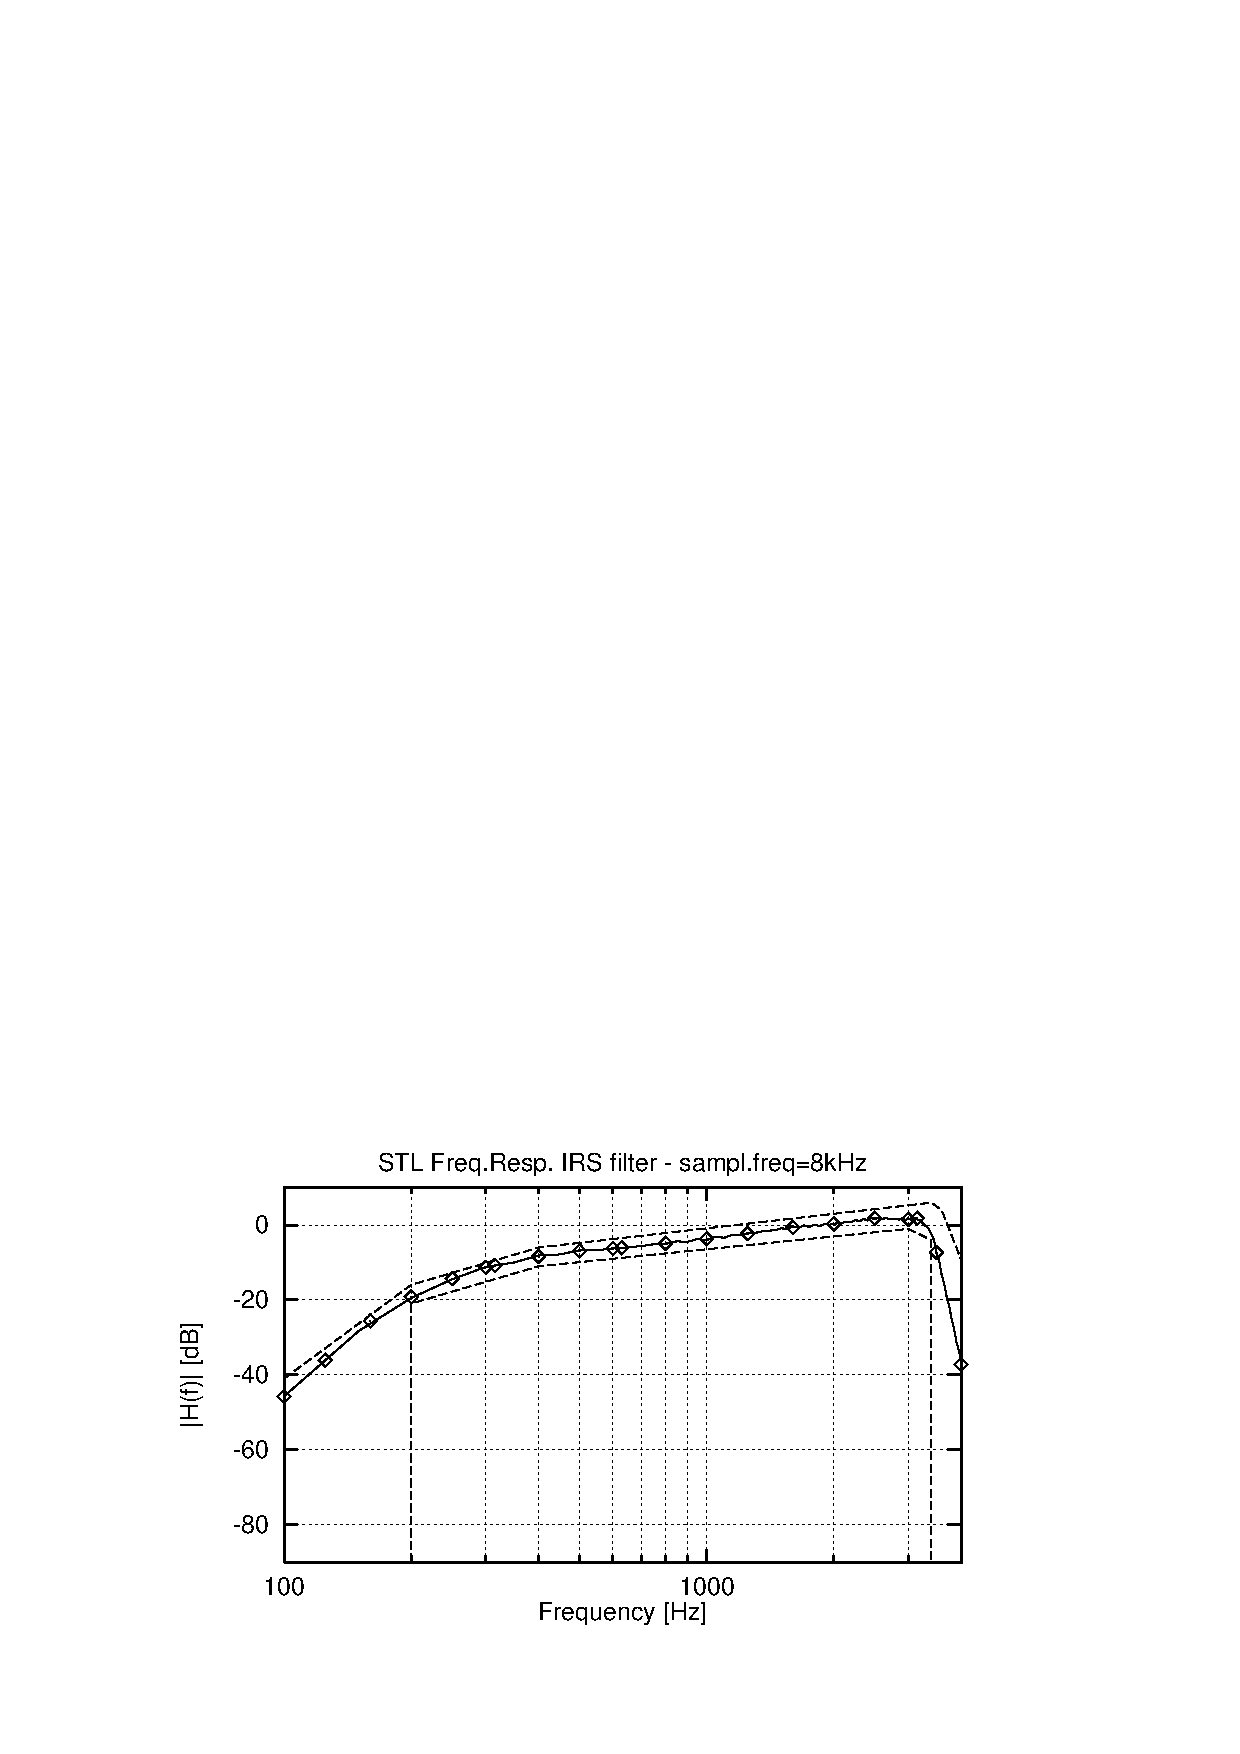
\includegraphics{irs_1_2}
 \\
   (a) Transmission-side IRS for input samples at 8 kHz.

 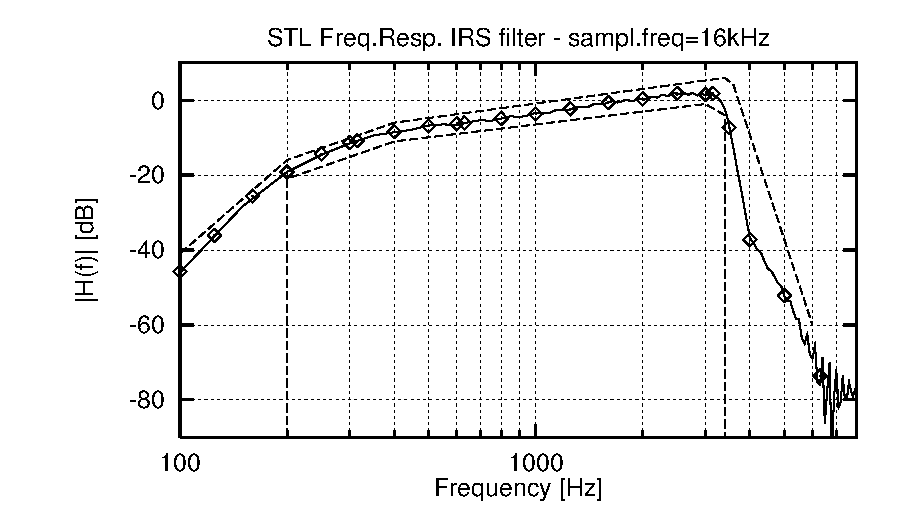
\includegraphics{irs_2_1}
    \\
   (b) Transmission-side IRS for input samples at 16 kHz.

  \end{center}
  \caption{\SF Transmission-side IRS filter responses.
               The diamonds represent the nominal values of the
               ``full'' IRS characteristic and the interrupted line
               represent the mask of the ``full'' IRS, as shown in
               figure 2 of ITU-T Rec. P.48.
               \label{tx-reg-irs-frq}}
\end{figure}
%------------------ End of regular IRS filters response ------------------


%-- Begin of FIR filters response: impulse response for regular IRS filters --
%Box dimension: 16.05cm x 18.03cm
\begin{figure}[hbtp]
  \begin{center}
     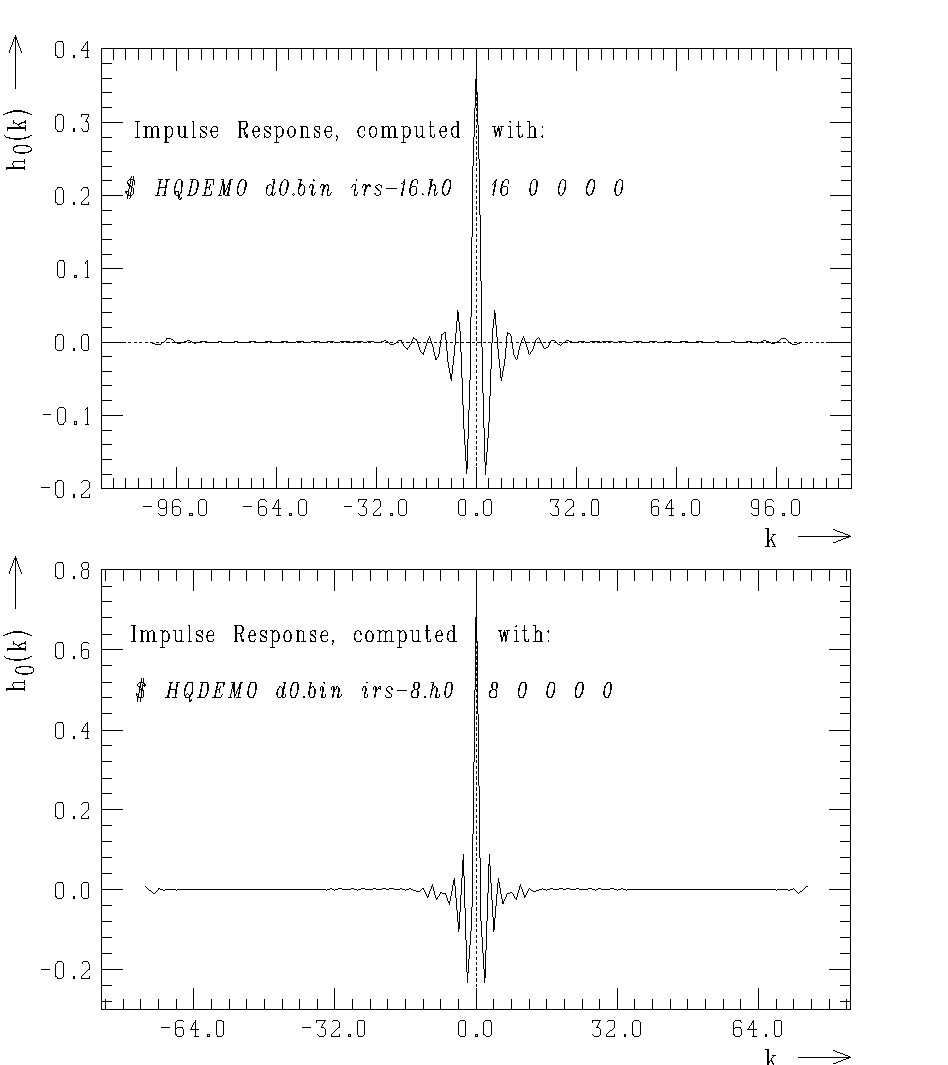
\includegraphics{irs-h0}
  \end{center}
  \caption{\SF Impulse response of transmission-side IRS filters
               at 16 and 8 kHz. \label{tx-reg-irs-ir}
          }
\end{figure}
%-- End of FIR filters response: impulse response for regular IRS filters --


%--------------- Begin of modified IRS TX filters response -----------------
\begin{figure}[hbtp]
  \begin{center}
     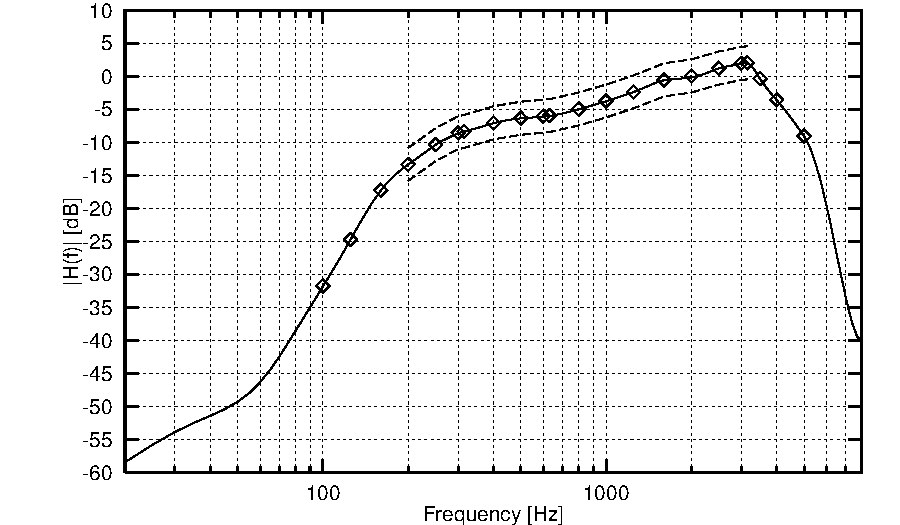
\includegraphics{mirs-16k}
     \\
   (a) Transmission-side modified IRS for input samples at 16 kHz.

     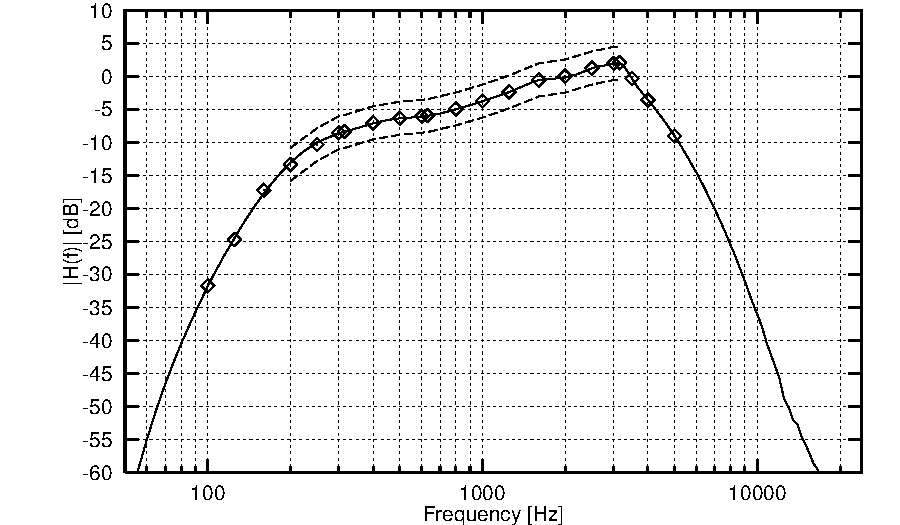
\includegraphics{mirs-48k}
    \\
   (b) Transmission-side modified IRS for input samples at 48 kHz.

  \end{center}
  \caption{\SF Transmission-side modified IRS filter responses. The
               interrupted line represents the mask of the ``full'' IRS.
               \label{tx-mod-irs-frq}}
\end{figure}
%------------------ End of modified IRS TX filters response -----------------


%-- Begin of FIR filters response: impulse response for mod IRS TX filters --
\begin{figure}[hbtp]
  \begin{center}
     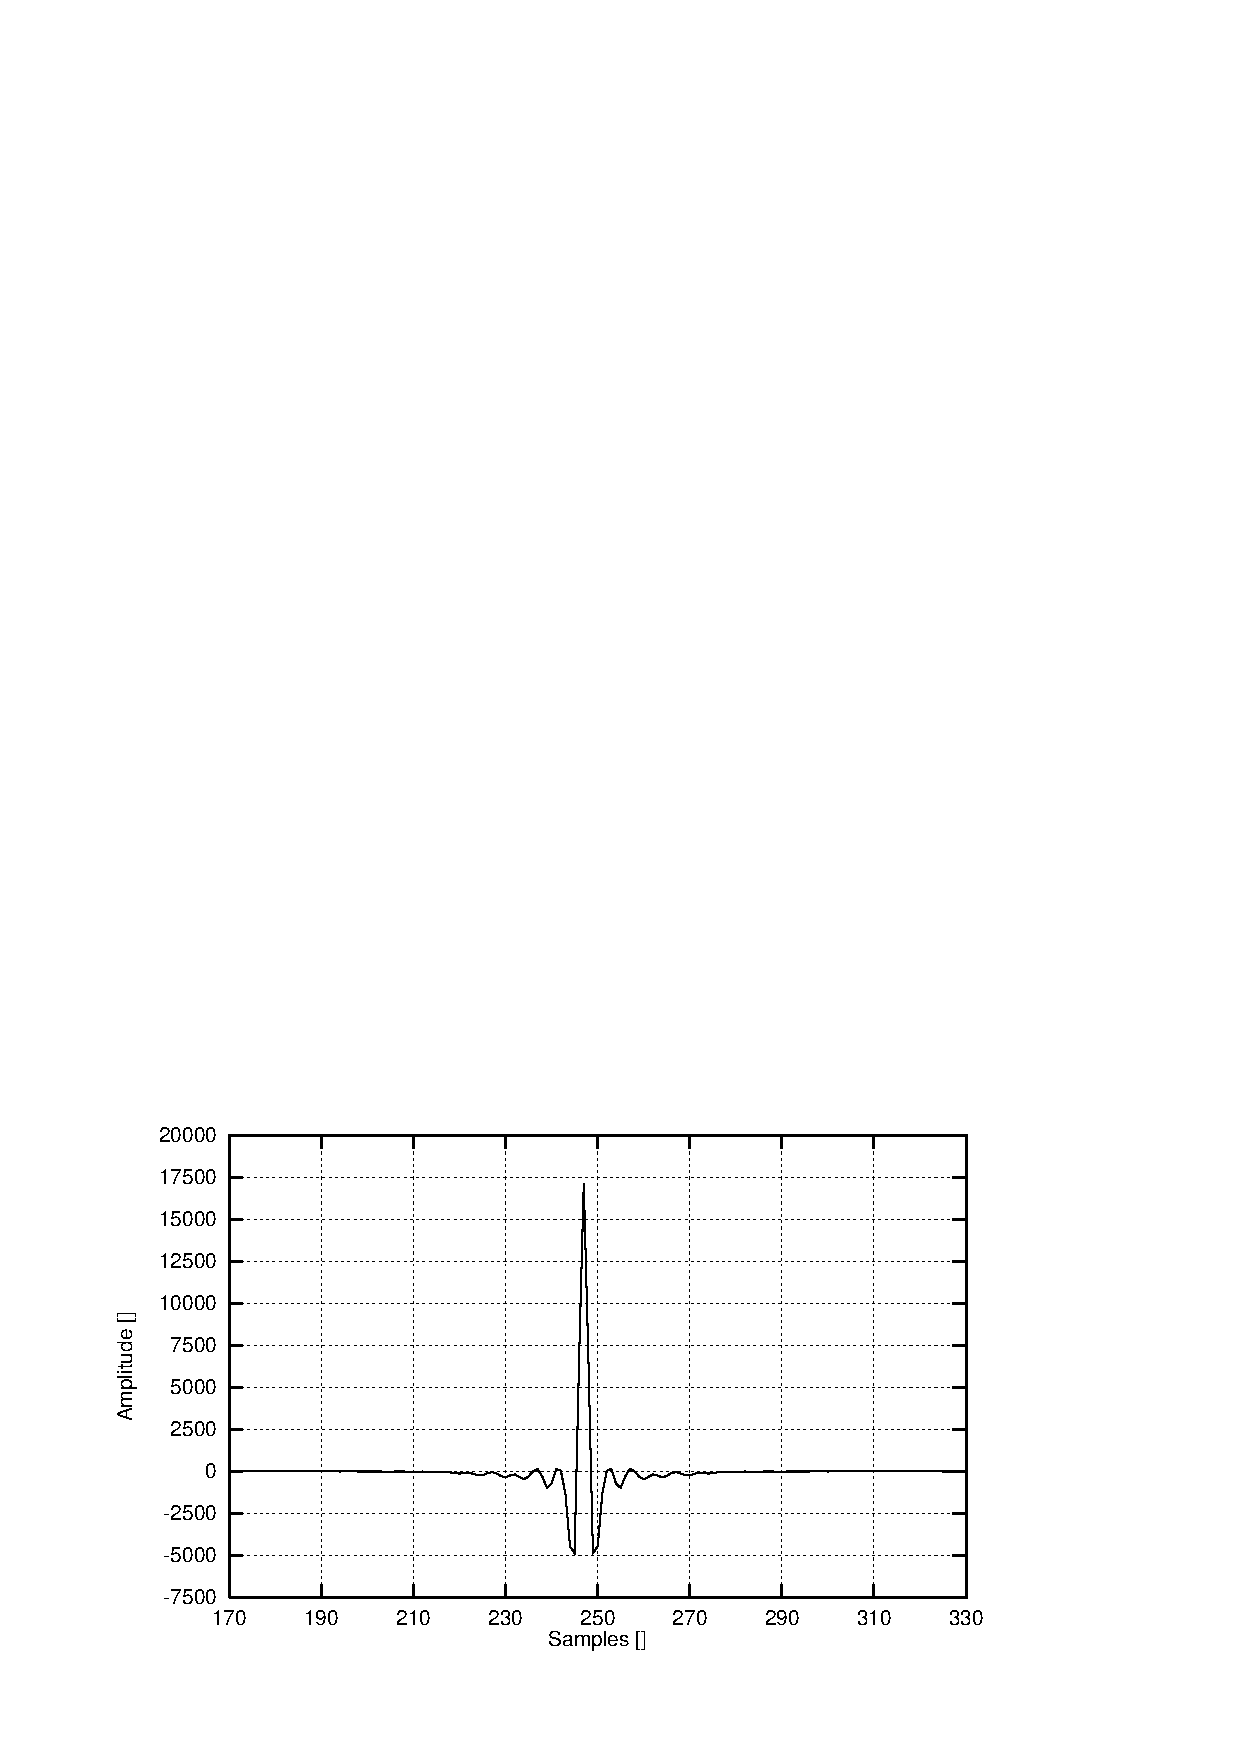
\includegraphics{mirs16-h0}
    \\
   (a) Transmission-side modified IRS for input samples at 16 kHz.

     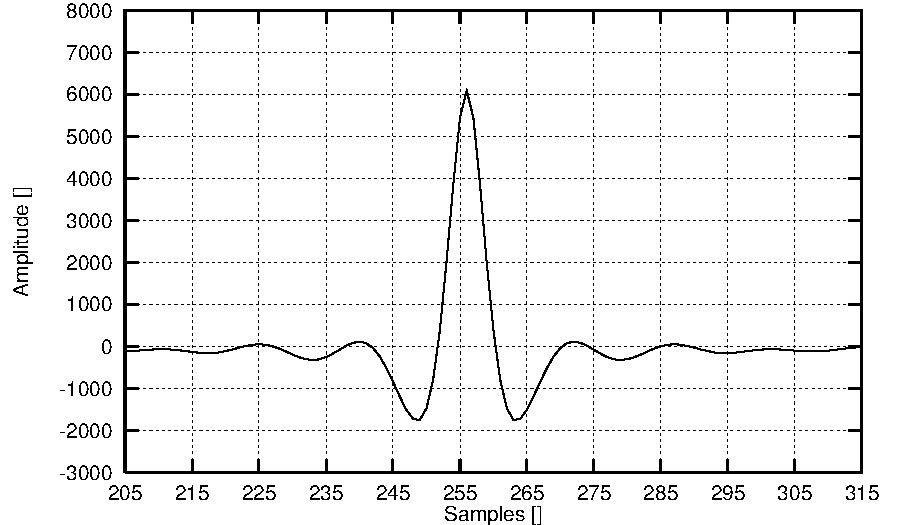
\includegraphics{mirs48-h0}
    \\
   (b) Transmission-side modified IRS for input samples at 48 kHz.

  \end{center}
  \caption{\SF Impulse response of transmission-side modified IRS filters
               at 16 kHz and 48 kHz. \label{tx-mod-irs-ir}
          }
\end{figure}
%----- End of FIR filters response: impulse response for IRS TX filters ------


%----------------- Begin of modified IRS RX filters response ----------------
\begin{figure}[hbtp]
  \begin{center}
    %Both boxes' dimension: 13.86cm x  7.30cm
     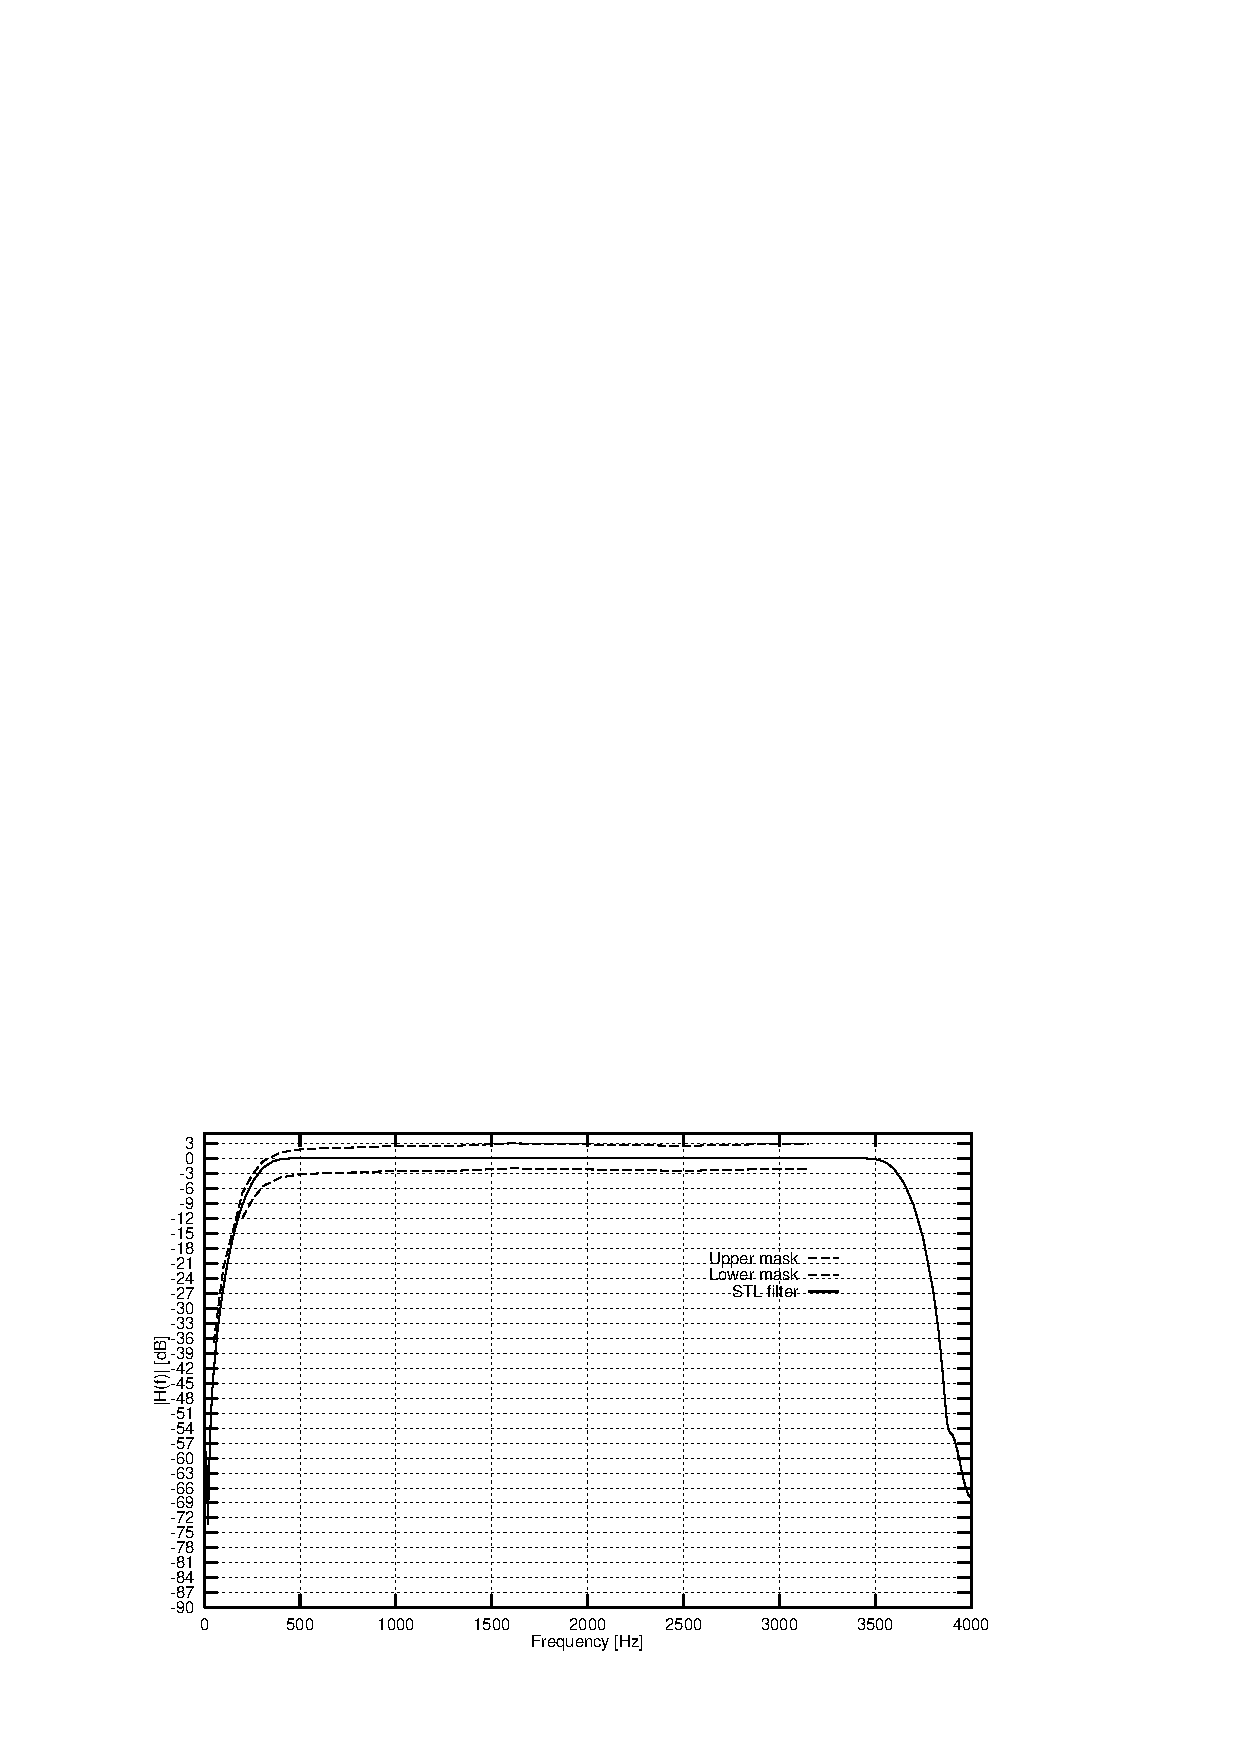
\includegraphics{rxirs08}
    \\
   (a) Receive-side modified IRS for input samples at 8 kHz.

     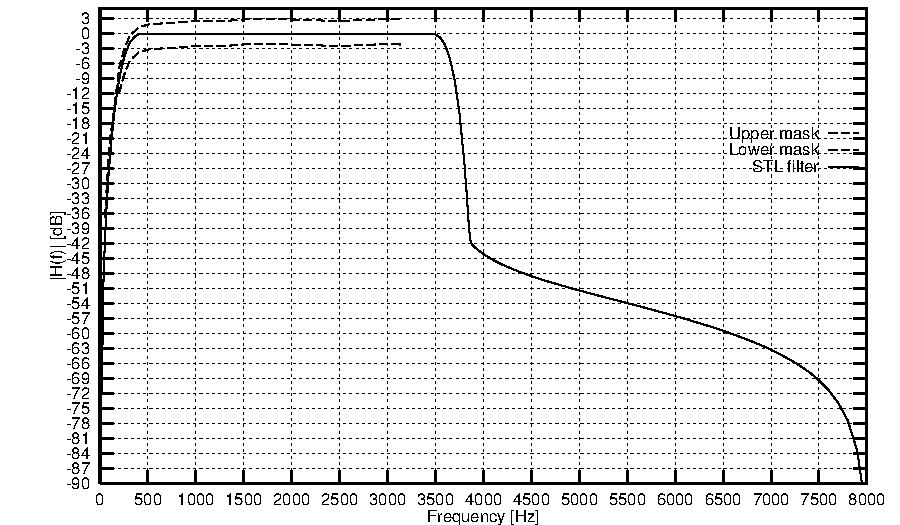
\includegraphics{rxirs16}
    \\
   (b) Receive-side modified IRS for input samples at 16 kHz.

  \end{center}
  \caption{\SF Receive-side modified IRS filter responses.
               The diamonds represent the nominal values of the
               modified IRS characteristic and the interrupted line
               represent the mask of the ``full'' IRS.
               \label{rx-mod-irs-frq}}
\end{figure}
%------------------ End of modified IRS RX filters response ----------------

\flushfloats
%-- Begin of FIR filters response: impulse response for mod IRS RX filters --
\begin{figure}[hbtp]
  \begin{center}
     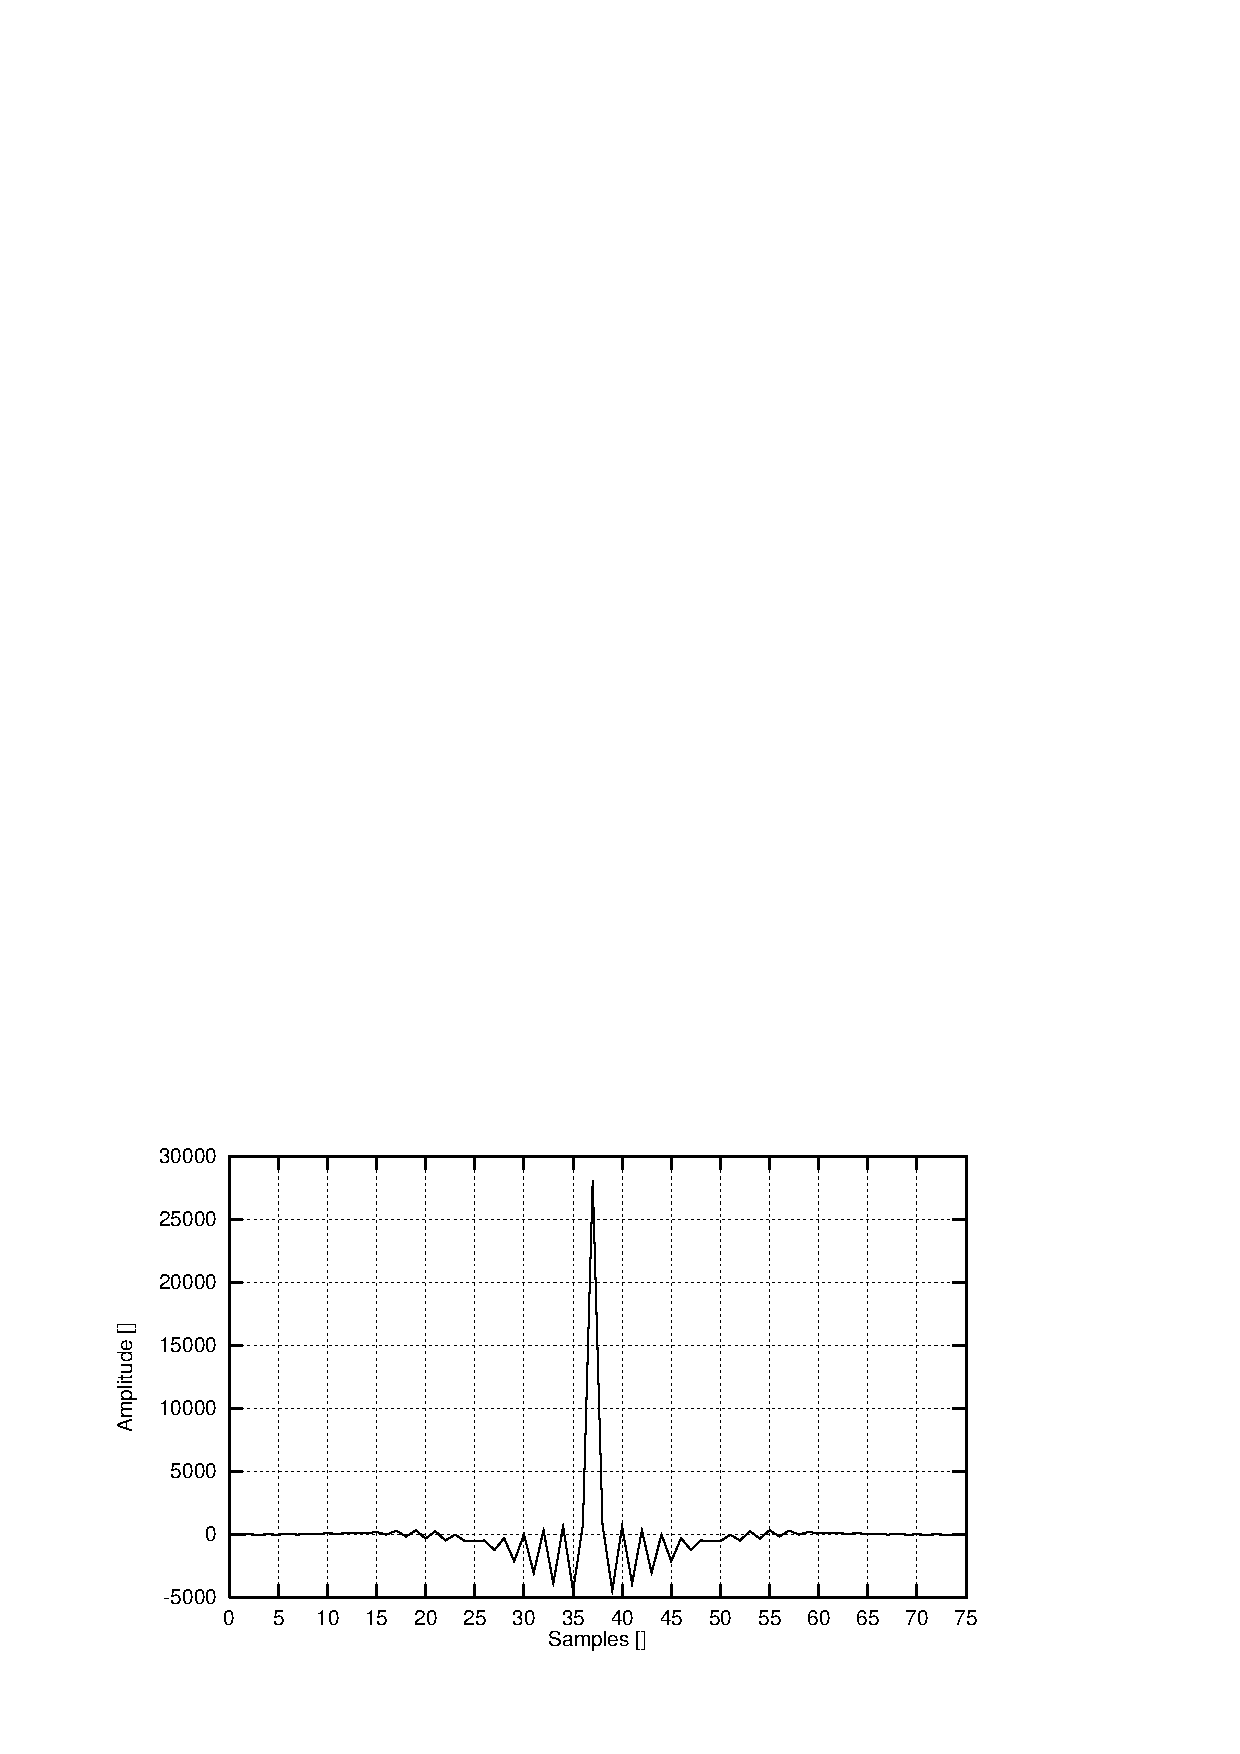
\includegraphics{rxirs08-h0}
    \\
   (a) Receive-side modified IRS for input samples at 8 kHz.

     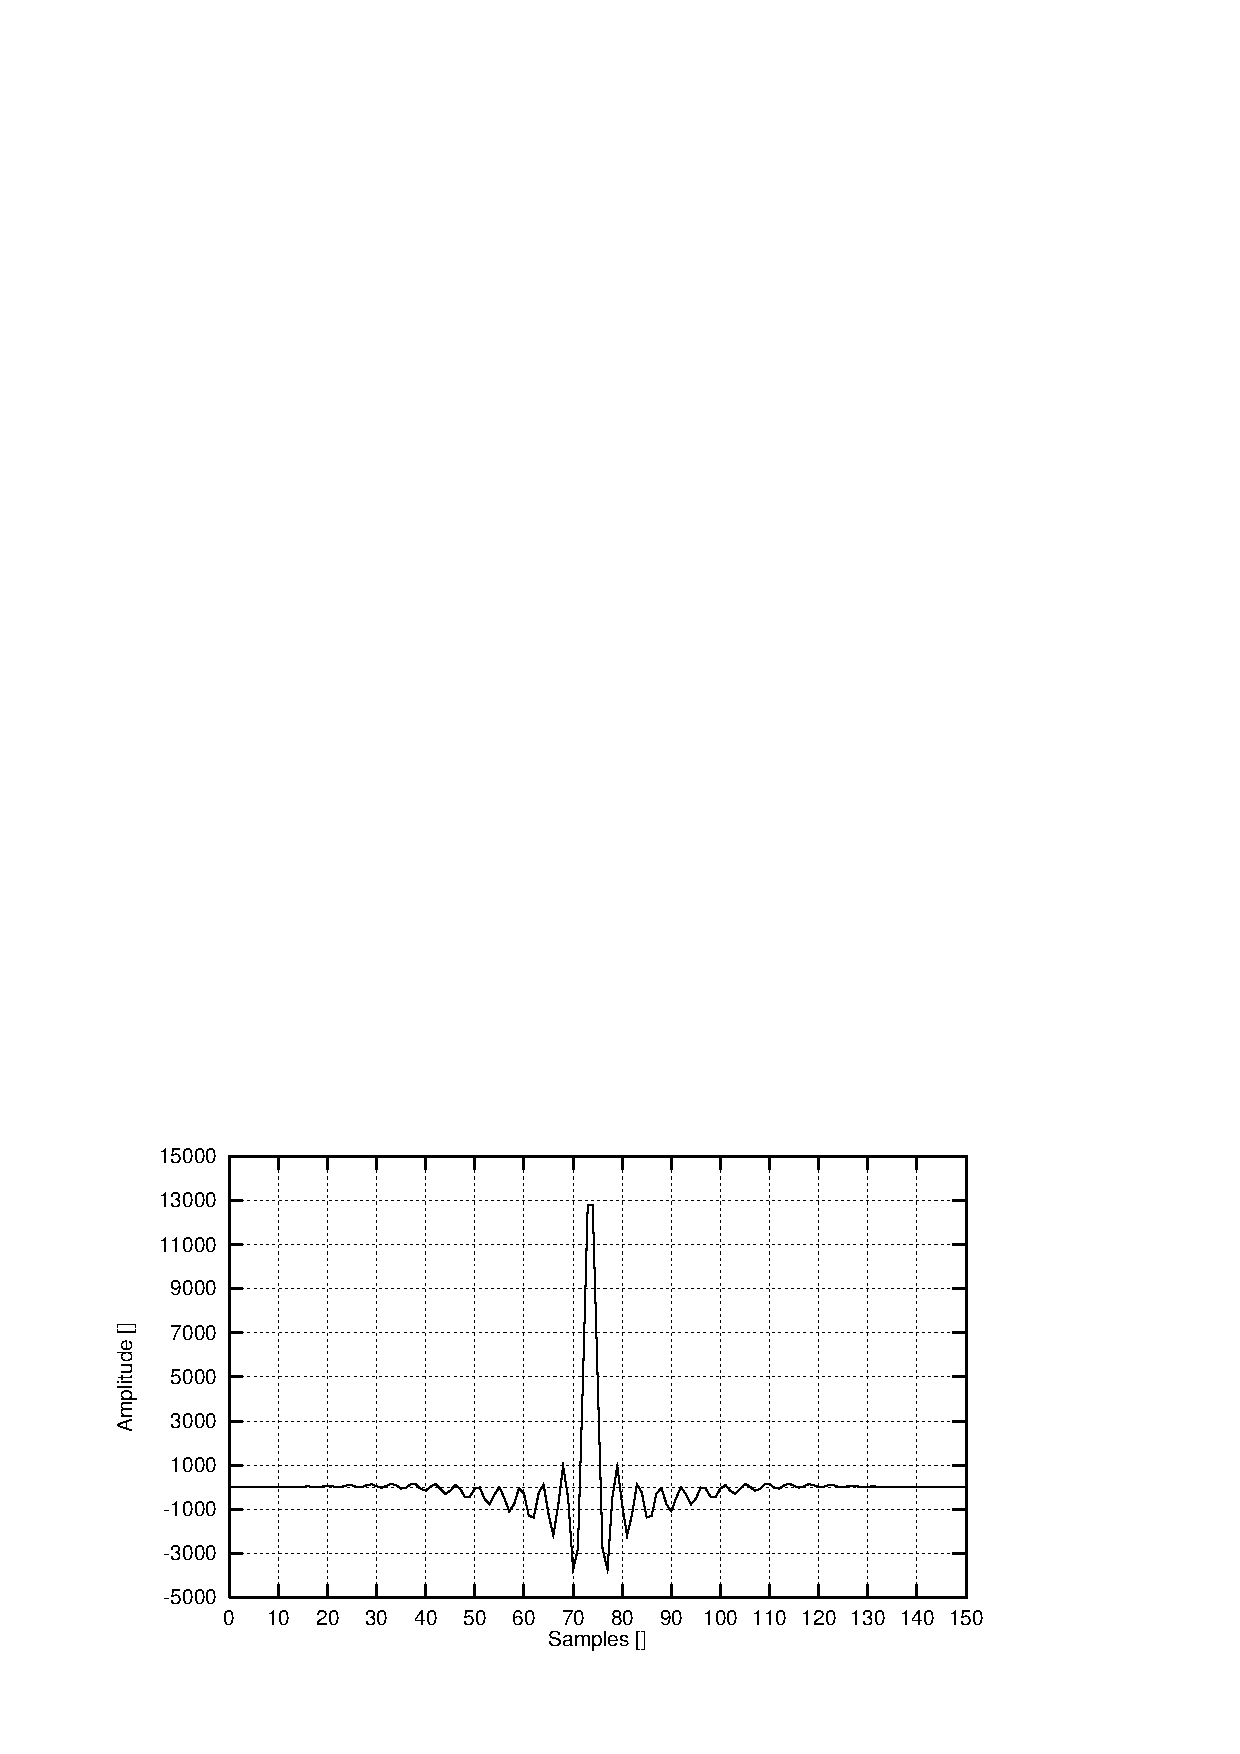
\includegraphics{rxirs16-h0}
    \\
   (b) Receive-side modified IRS for input samples at 16 kHz.

  \end{center}
  \caption{\SF Impulse response of receive-side modified IRS filters at 8 kHz
               (top) and 16 kHz (bottom). \label{rx-mod-irs-ir}
          }
\end{figure}
%--- End of FIR filters response: impulse response for RX mod IRS filters ---


%----------- Begin of FIR filters response: frq for psophometric filter  ----
\begin{figure}[hbtp]
  \begin{center}
 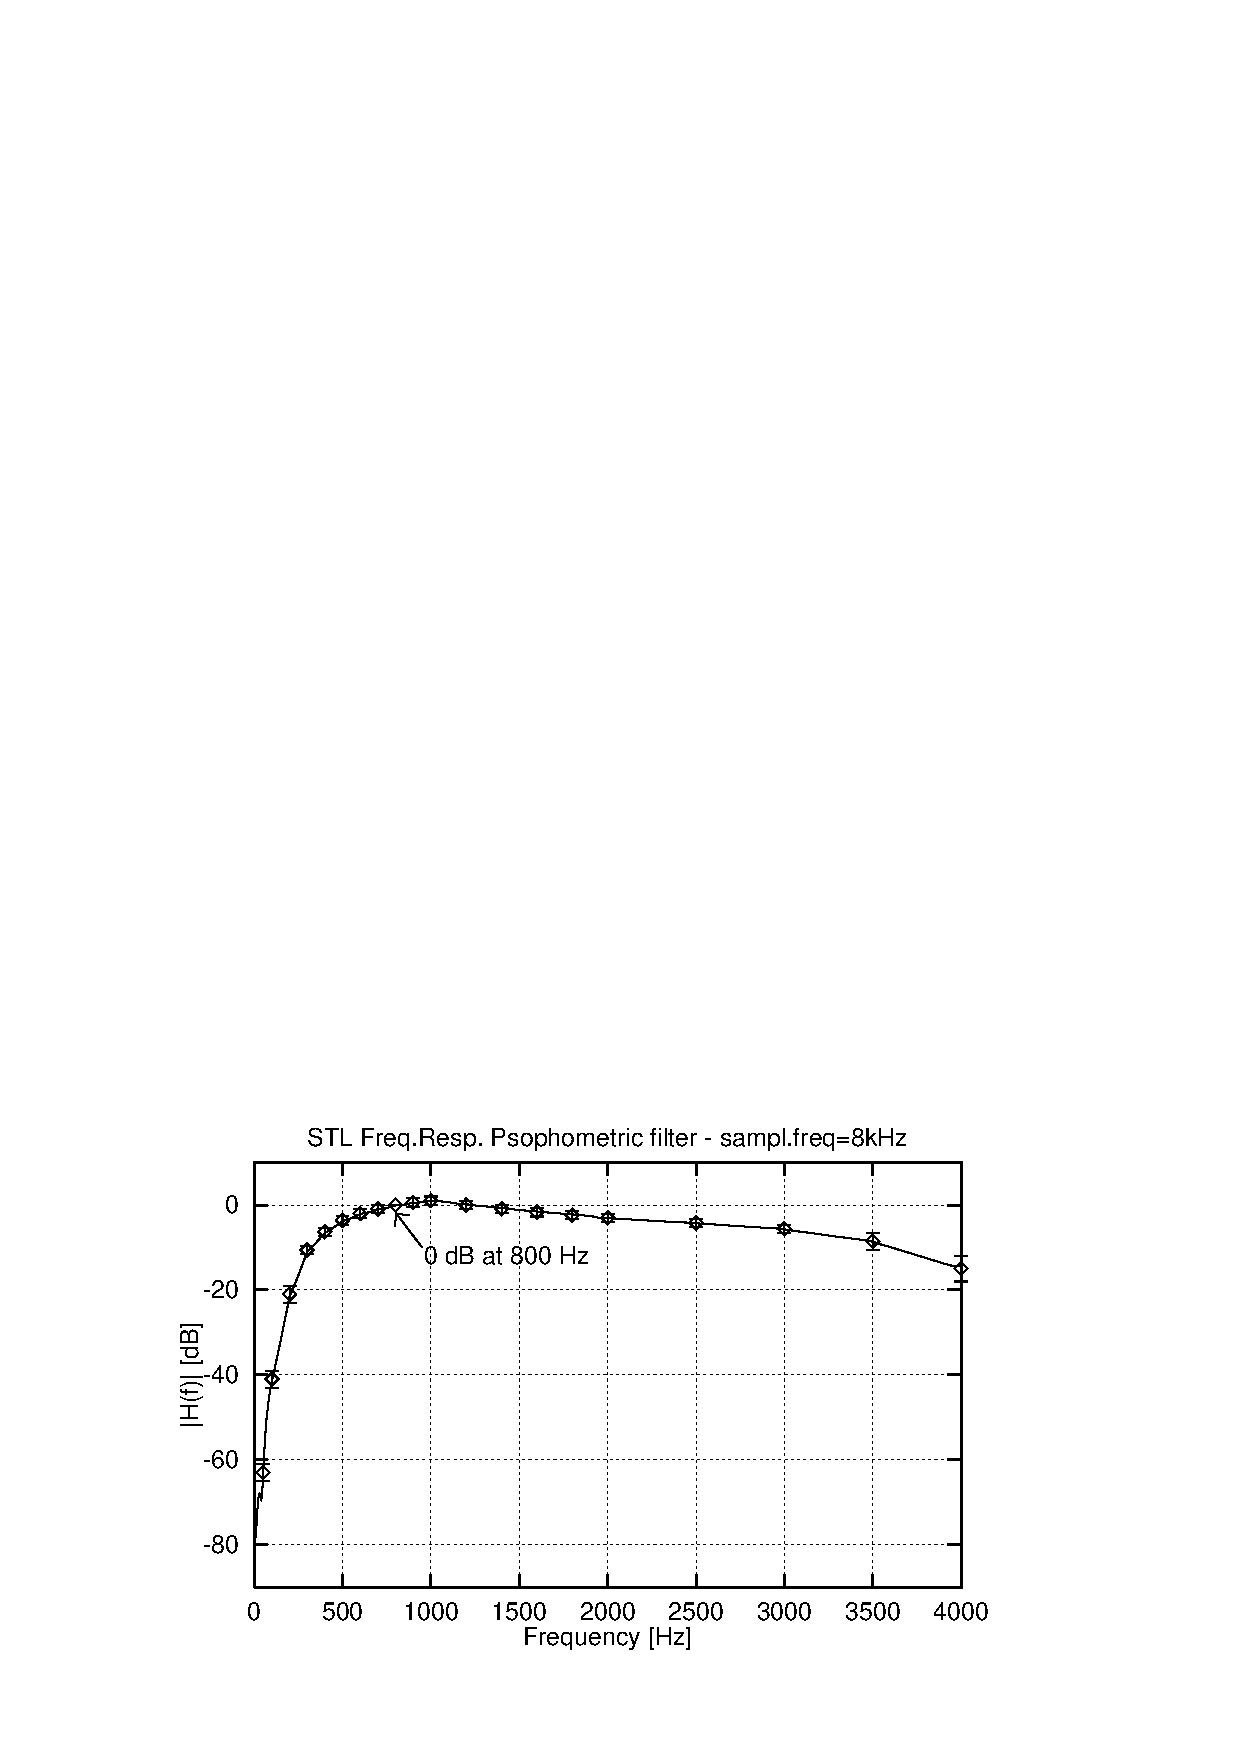
\includegraphics{pso_8k}
  \end{center}
  \caption{\SF Frequency response for the psophometric filter. The
               points show the average points and the allowed range as per
               ITU-T Rec. O.41.
               \label{pso-08k-frq}
          }

\end{figure}
%------------- End of FIR filters response: frq for psophometric -------------


%----------- Begin of FIR filters response: frq for deltasm filter  ----
\begin{figure}[hbtp]
  \begin{center}
 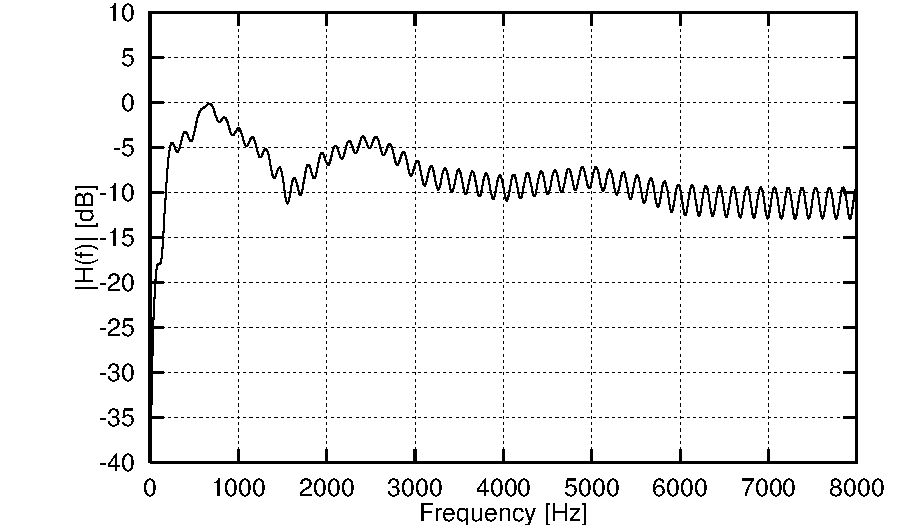
\includegraphics{dsm_16k}

  \end{center}
  \caption{\SF Frequency response for the $\Delta_{SM}$ filter.
               \label{delta-sm-frq}
          }

\end{figure}
%------------- End of FIR filters response: frq for deltasm -------------


%----------- Begin of FIR filters response: frq for P.341 filter  --------
\begin{figure}[hbtp]
  \begin{center}
 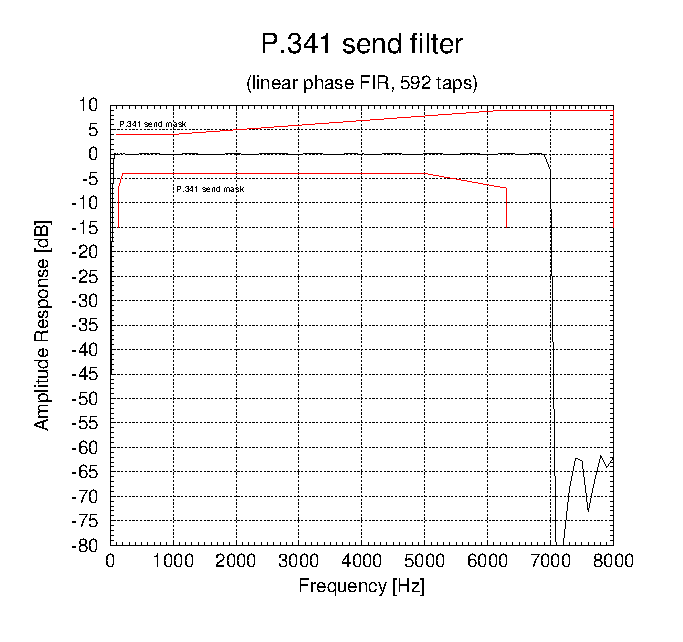
\includegraphics{p341}
  \end{center}
  \caption{\SF STL P.341 send-side filter frequency response for data
               sampled at 16 kHz (factor 1:1).
           \label{tx-p341-frq}
          }
\end{figure}
%------------- End of FIR filters response: frq for P.341 ----------------


%--- Begin of FIR filters response: impulse response for P.341 --------
\begin{figure}[hbtp]
  \begin{center}
 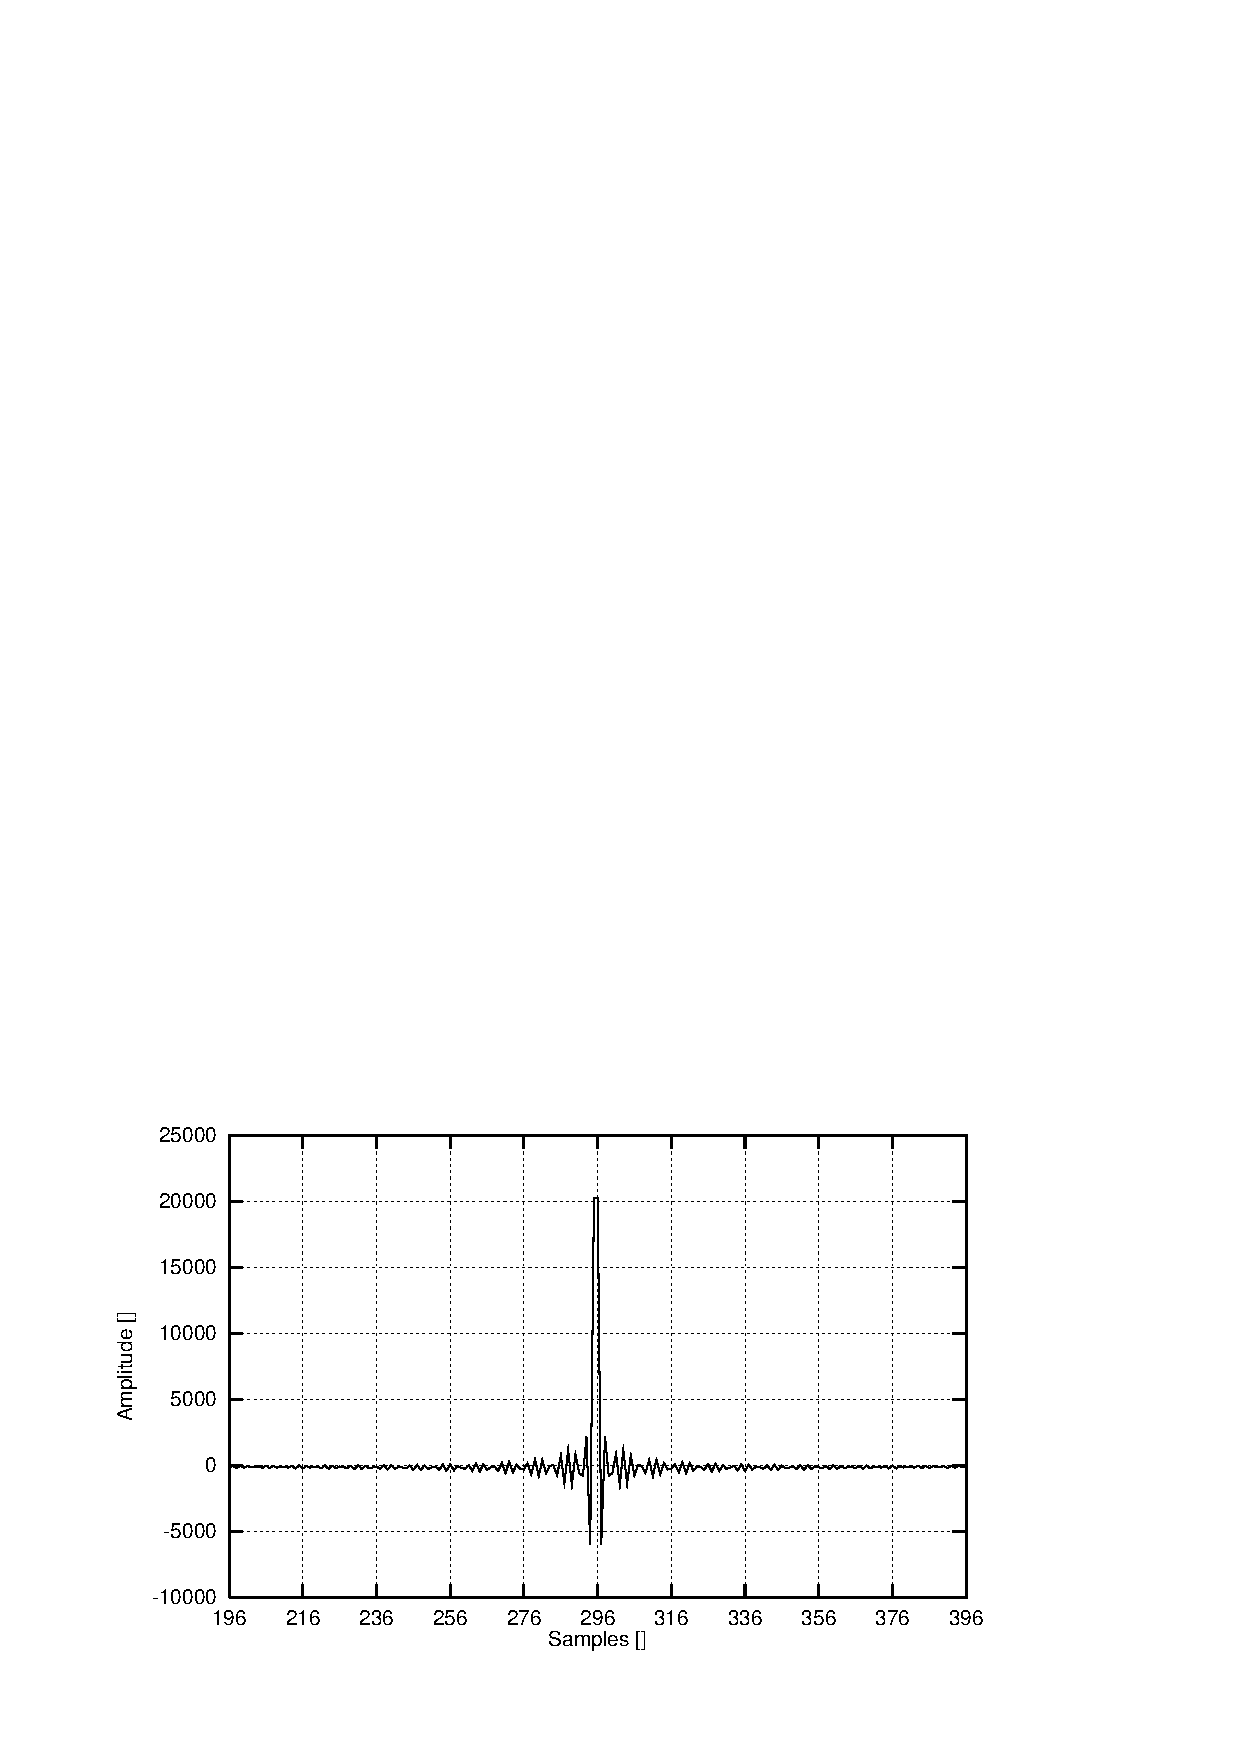
\includegraphics{p341-h0}
  \end{center}
  \caption{\SF STL P.341 send-side filter impulse response.
           \label{tx-p341-ir}
          }
\end{figure}
%----- End of FIR filters response: impulse response for P.341 -----


%----------- Begin of FIR filters response: frq for 50 Hz-14 kHz BP filter  ----
\begin{figure}[hbtp]
  \begin{center}
  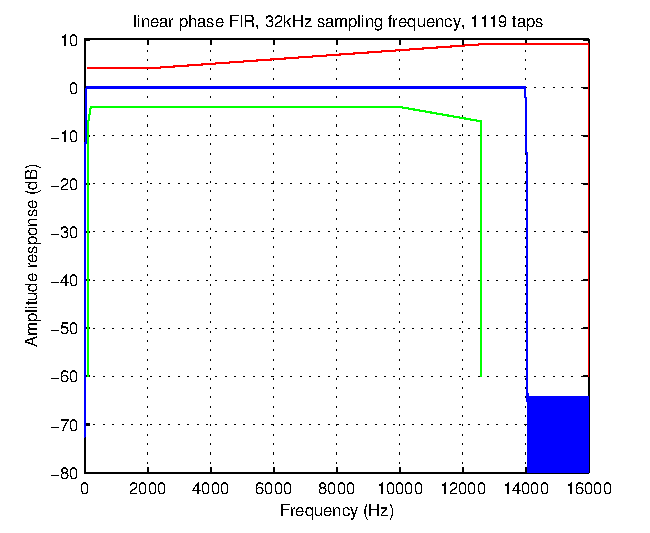
\includegraphics{50-14K}
  \end{center}
  \caption{\SF STL 50 Hz - 14 kHz band limiting filter frequency response for data
               sampled at 32 kHz (factor 1:1).
           \label{50_14k-32k-frq}
          }
\end{figure}
%------------- End of FIR filters response: frq for 50 Hz-14 kHz BP -------------


%--- Begin of FIR filters response: impulse response for 50 Hz - 14 kHz BP --------
\begin{figure}[hbtp]
  \begin{center}
 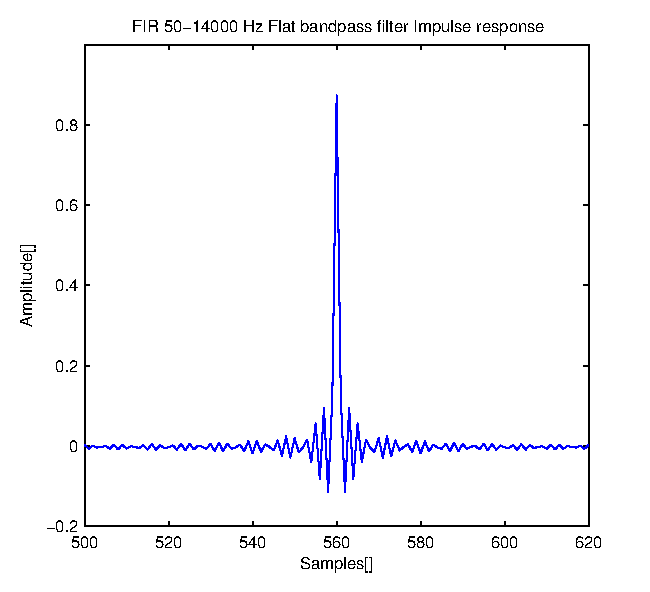
\includegraphics{50-14K-h0}
  \end{center}
  \caption{\SF STL 50 Hz - 14 kHz band limiting filter impulse response.
           \label{50_14k-32k-ir}
          }
\end{figure}
%----- End of FIR filters response: impulse response for 50 Hz - 14 kHz BP -----

\clearpage
\newpage


%%PROBLEM
%----------- Begin of FIR filters response: frq for 50 Hz - 5 kHz BP filter  ----
\begin{figure}[hbtp]
  \begin{center}
 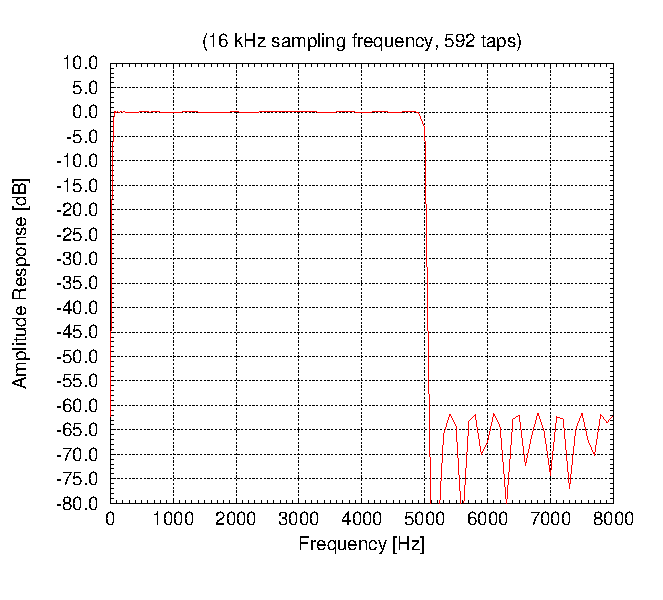
\includegraphics{bp5k}

  \end{center}
  \caption{\SF STL 50 Hz - 5 kHz band limiting filter frequency response for data
               sampled at 16 kHz (factor 1:1).
           \label{bp5k-16k-frq}
          }
\end{figure}
%------------- End of FIR filters response: frq for 50 Hz - 5 kHz BP -------------


%--- Begin of FIR filters response: impulse response for 50 Hz - 5 kHz BP --------
\begin{figure}[h!btp]
  \begin{center}
 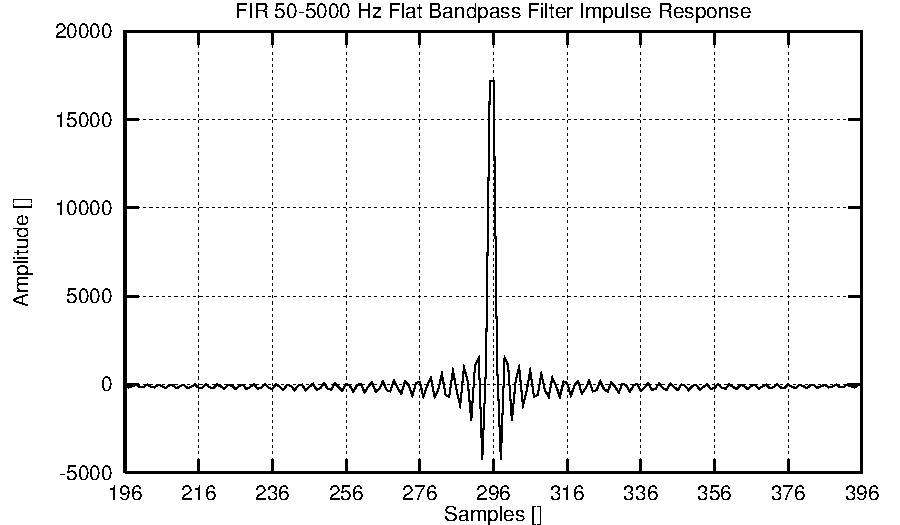
\includegraphics{bp5k-h0}
  \end{center}
  \caption{\SF STL 50 Hz - 5 kHz band limiting filter impulse response.
           \label{bp5k-16k-ir}
          }
\end{figure}
%----- End of FIR filters response: impulse response for 50 Hz - 5 kHz BP -----


%----------- Begin of FIR filters response: frq for 100 Hz - 5 kHz BP filter  ----
\begin{figure}[hbtp]
  \begin{center}
 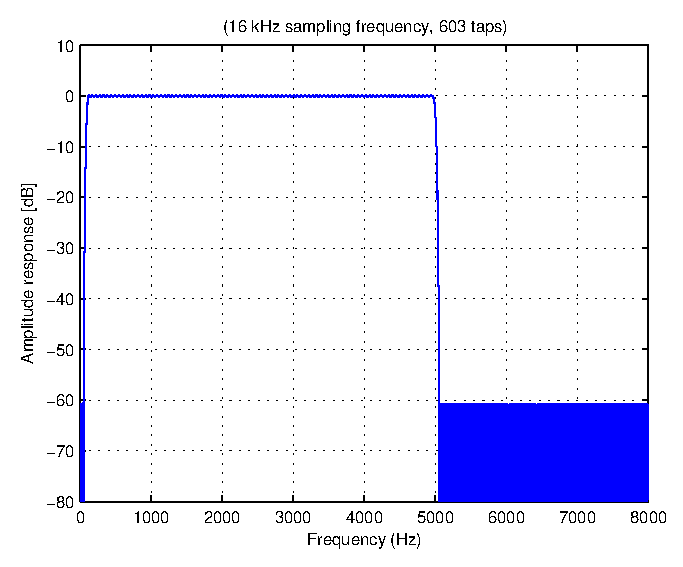
\includegraphics{bp100_5k}
  \end{center}
  \caption{\SF STL 100 Hz - 5 kHz band limiting filter frequency response for data
               sampled at 16 kHz (factor 1:1).
           \label{bp100_5k-16k-frq}
          }
\end{figure}
%------------- End of FIR filters response: frq for 100 Hz - 5 kHz BP -------------


%--- Begin of FIR filters response: impulse response for 100 Hz - 5 kHz BP --------
\begin{figure}[hbtp]
  \begin{center}
 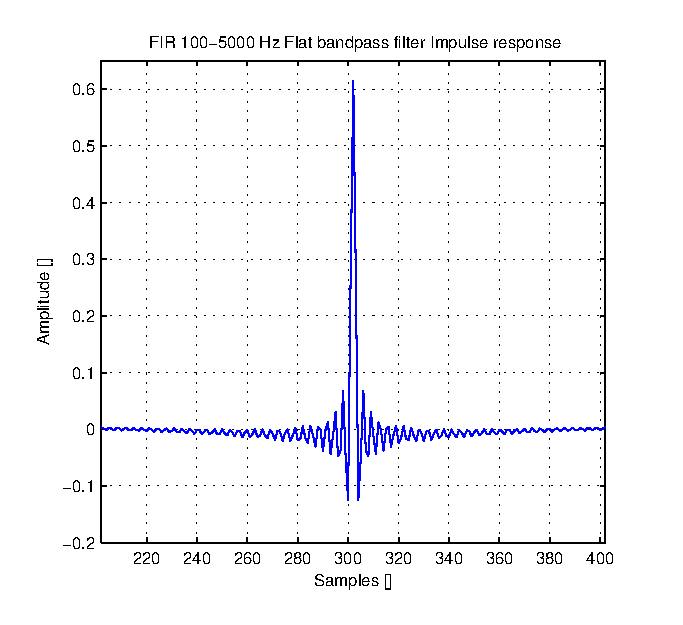
\includegraphics{bp100_5k-h0}
  \end{center}
  \caption{\SF STL 100 Hz - 5 kHz band limiting filter impulse response.
           \label{bp100_5k-16k-ir}
          }
\end{figure}
%----- End of FIR filters response: impulse response for 100 Hz-5 kHz BP -----


%----------- Begin of FIR filters response: frq for 20 Hz - 20 kHz BP filter  ----
\begin{figure}[h]
  \begin{center}
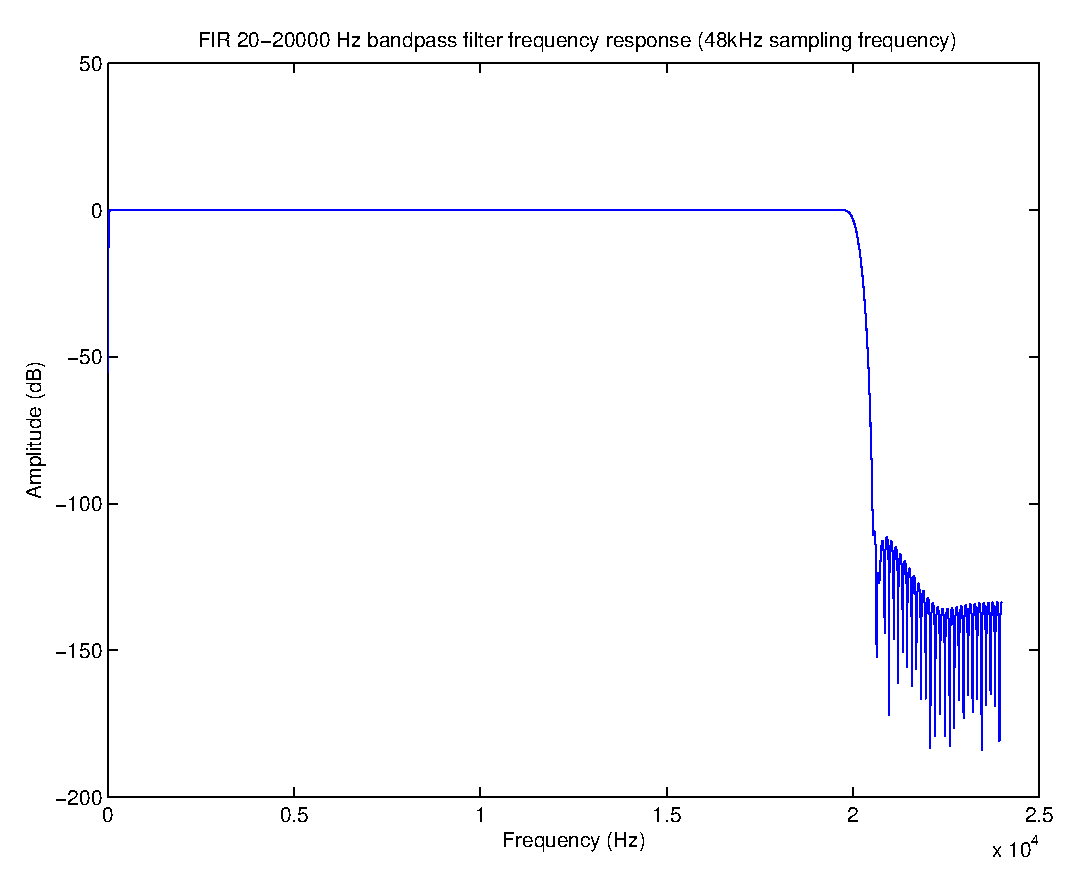
\includegraphics[scale=0.7]{bp20_20k}
  \end{center}
  \caption{\SF STL 20 Hz - 20 kHz band limiting filter frequency response for data
               sampled at 48 kHz (factor 1:1).
           \label{bp20_20k-48k-frq}
          }
\end{figure}
%------------- End of FIR filters response: frq for 20 Hz - 20 kHz BP -------------


%--- Begin of FIR filters response: impulse response for 20 Hz - 20 kHz BP --------
\begin{figure}[b]
  \begin{center}
 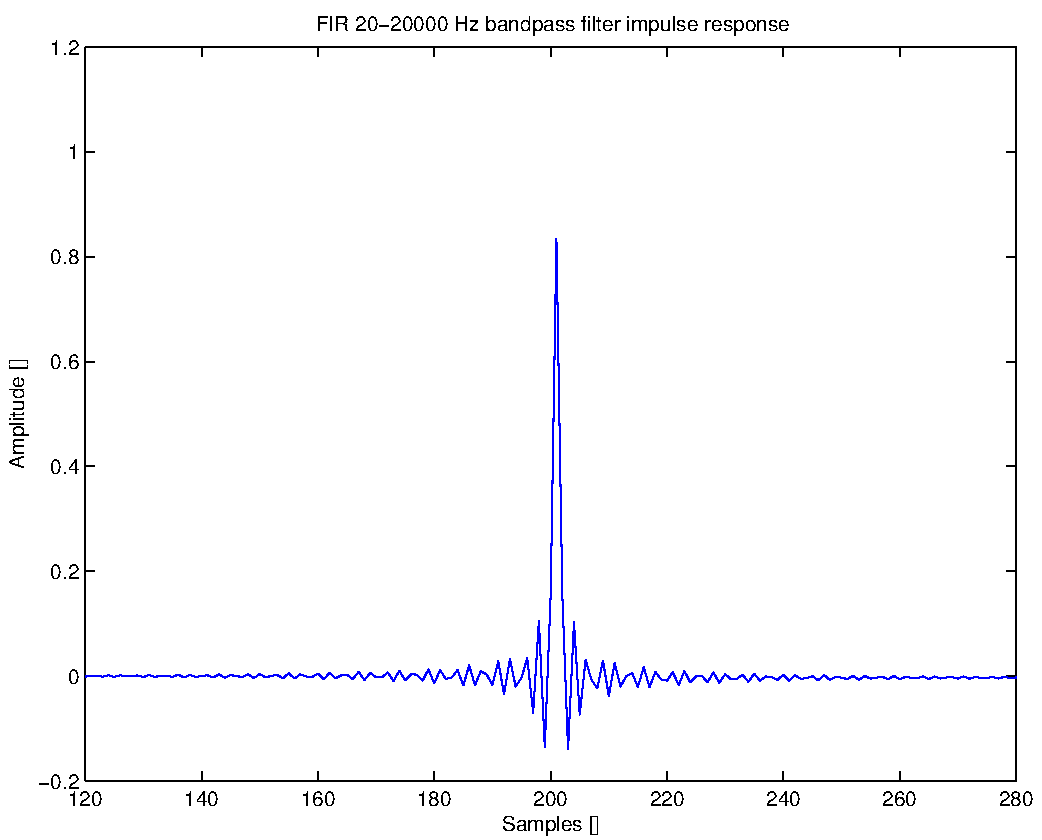
\includegraphics[scale=0.7]{bp20_20k-h0}
  \end{center}
  \caption{\SF STL 20 Hz - 20 kHz band limiting filter impulse response, (the complete impulse response is of length 4001).
           \label{bp20_20k-48k-ir}
          }
\end{figure}
%----- End of FIR filters response: impulse response for 20 Hz - 20 kHz BP -----


%----------- Begin of FIR filters response: frq for LP1p5 filter  ----
\begin{figure}[hbtp]
  \begin{center}
 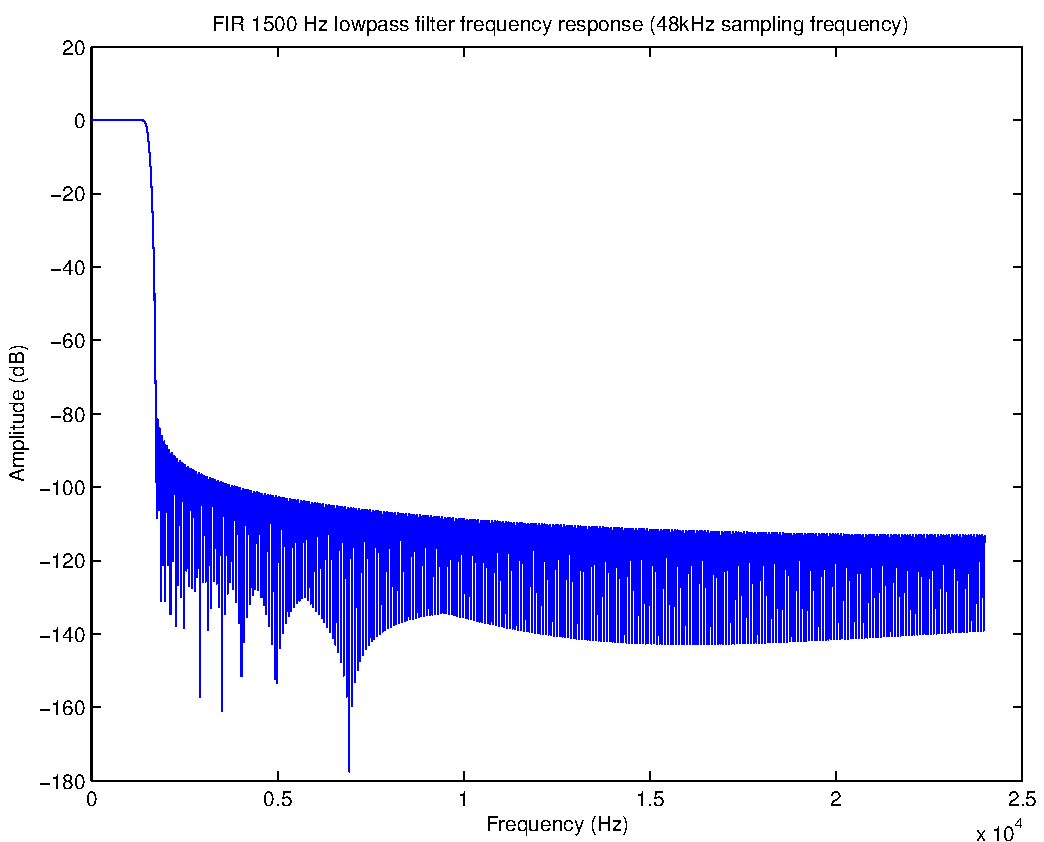
\includegraphics[scale=0.65]{LP1p5}
  \end{center}
  \caption{\SF Frequency response of the STL MUSHRA anchor LP1.5 -- Low-pass filter with cut-off frequency 1.5 kHz for a sampling frequency of 48 kHz (factor 1:1).
           \label{LP1p5-frq}
          }
\end{figure}
%------------- End of FIR filters response: frq for LP1p5 -------------

%--- Begin of FIR filters response: impulse response for LP1p5 --------
\begin{figure}[hbtp]
  \begin{center}
 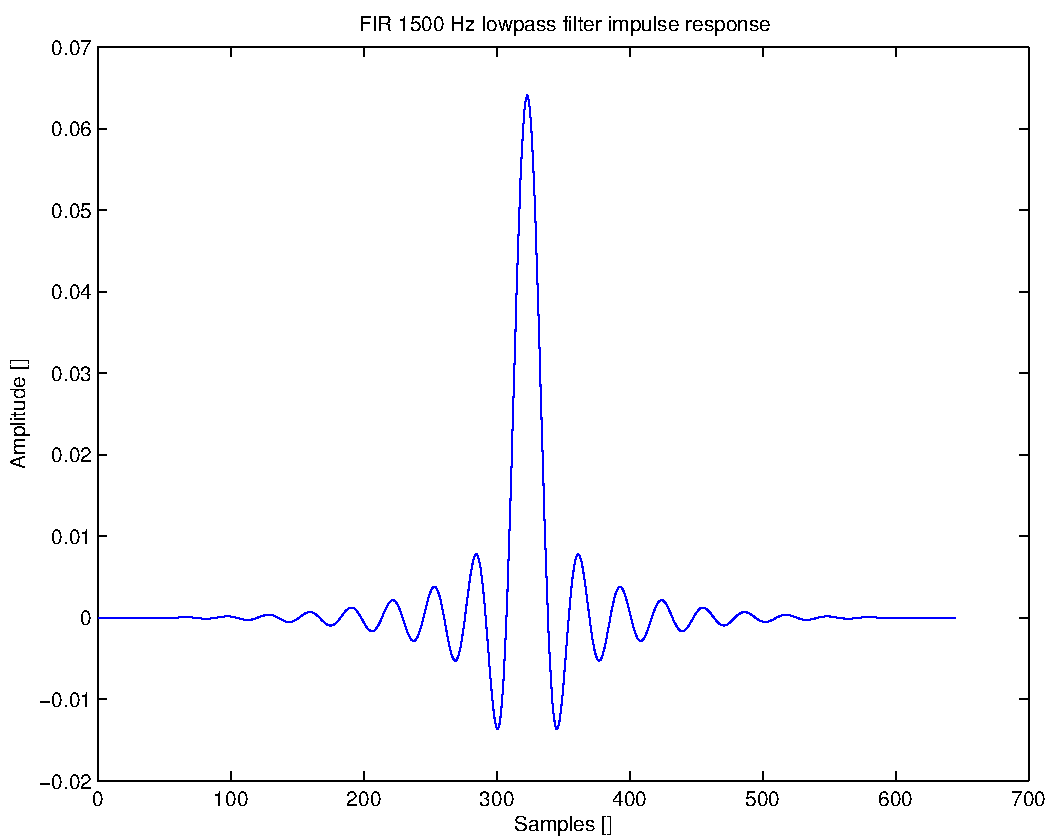
\includegraphics[scale=0.65]{LP1p5-h0}
  \end{center}
  \caption{\SF Impulse response of the STL MUSHRA anchor LP1.5 -- Low-pass filter with cut-off frequency 1.5 kHz for a sampling frequency of 48 kHz (factor 1:1).
           \label{LP1p5-ir}
          }
\end{figure}
%----- End of FIR filters response: impulse response for LP1p5 -----


%----------- Begin of FIR filters response: frq for LP35 filter  ----
\begin{figure}[hbtp]
  \begin{center}
 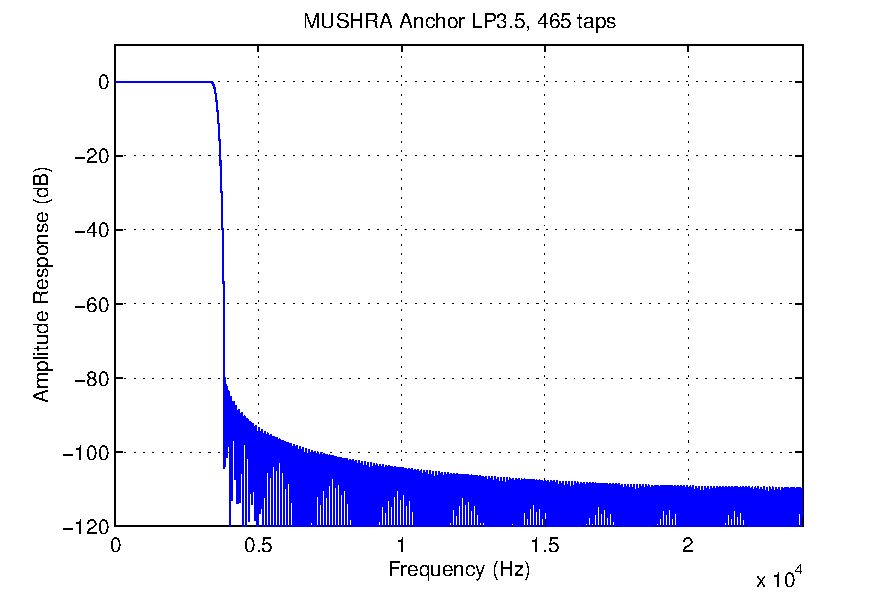
\includegraphics{LP35}
  \end{center}
  \caption{\SF Frequency response of the STL MUSHRA anchor LP3.5 -- Low-pass filter with cut-off frequency 3.5 kHz for a sampling frequency of 48 kHz (factor 1:1).
           \label{LP35-frq}
          }
\end{figure}
%------------- End of FIR filters response: frq for LP35 -------------

%--- Begin of FIR filters response: impulse response for LP35 --------
\begin{figure}[hbtp]
  \begin{center}
 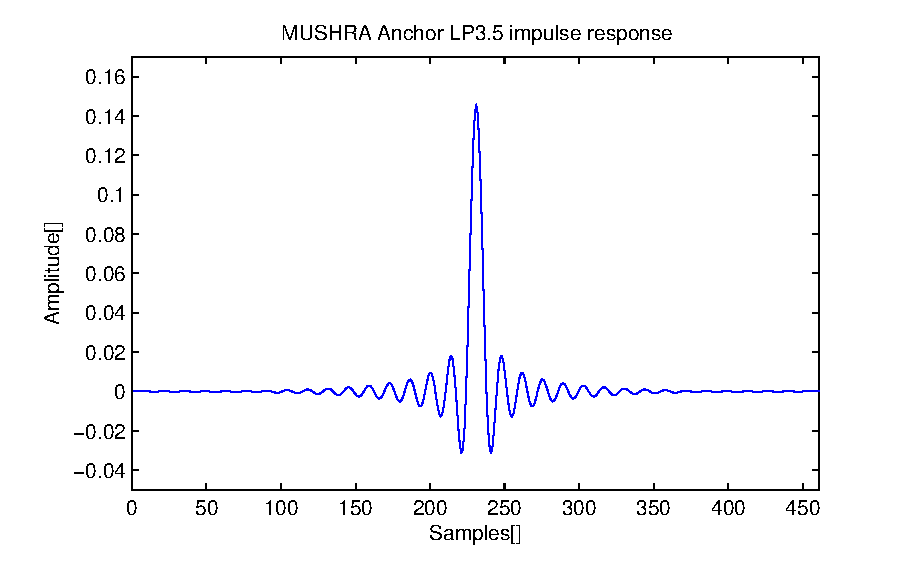
\includegraphics{LP35-h0}
  \end{center}
  \caption{\SF Impulse response of the STL MUSHRA anchor LP3.5 -- Low-pass filter with cut-off frequency 3.5 kHz for a sampling frequency of 48 kHz (factor 1:1).
           \label{LP35-ir}
          }
\end{figure}
%----- End of FIR filters response: impulse response for LP35 -----


%----------- Begin of FIR filters response: frq for LP7 filter  ----
\begin{figure}[hbtp]
  \begin{center}
 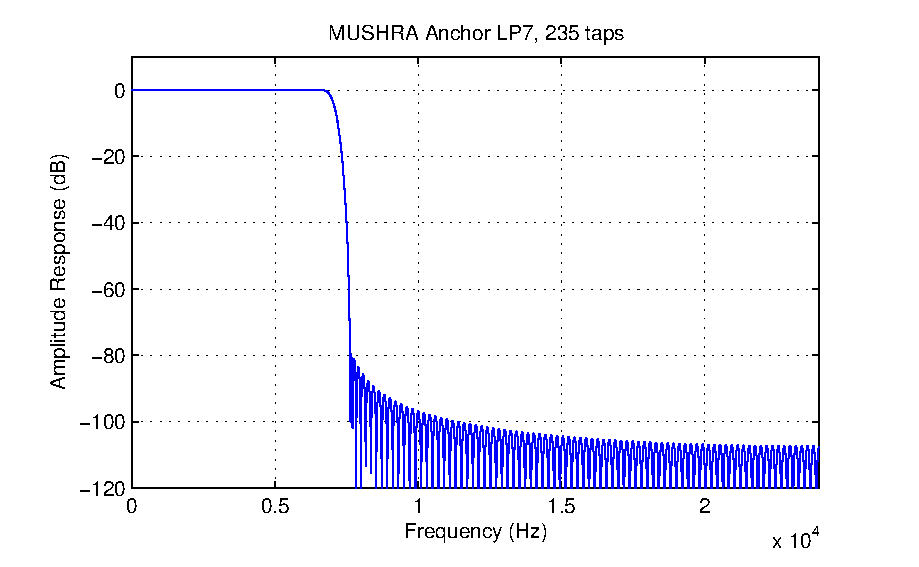
\includegraphics{LP7}
  \end{center}
  \caption{\SF Frequency response of the STL MUSHRA anchor LP7 -- Low-pass filter with cut-off frequency 7 kHz for a sampling frequency of 48 kHz (factor 1:1).
           \label{LP7-frq}
          }
\end{figure}
%------------- End of FIR filters response: frq for LP7 -------------


%--- Begin of FIR filters response: impulse response for LP7 --------
\begin{figure}[hbtp]
  \begin{center}
 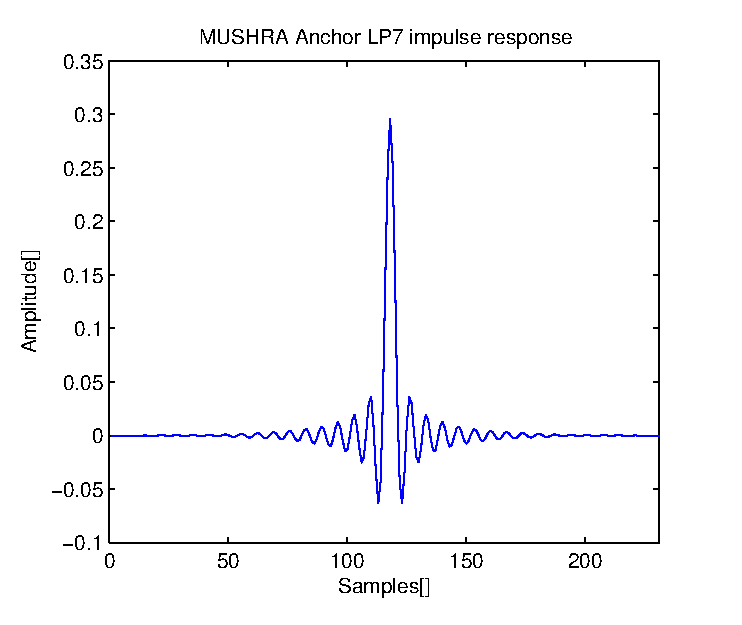
\includegraphics{LP7-h0}
  \end{center}
  \caption{\SF Impulse response of the STL MUSHRA anchor LP7 -- Low-pass filter with cut-off frequency 7 kHz for a sampling frequency of 48 kHz (factor 1:1).
           \label{LP7-ir}
          }
\end{figure}
%----- End of FIR filters response: impulse response for LP7 -----


%----------- Begin of FIR filters response: frq for LP10 filter  ----
\begin{figure}[hbtp]
  \begin{center}
 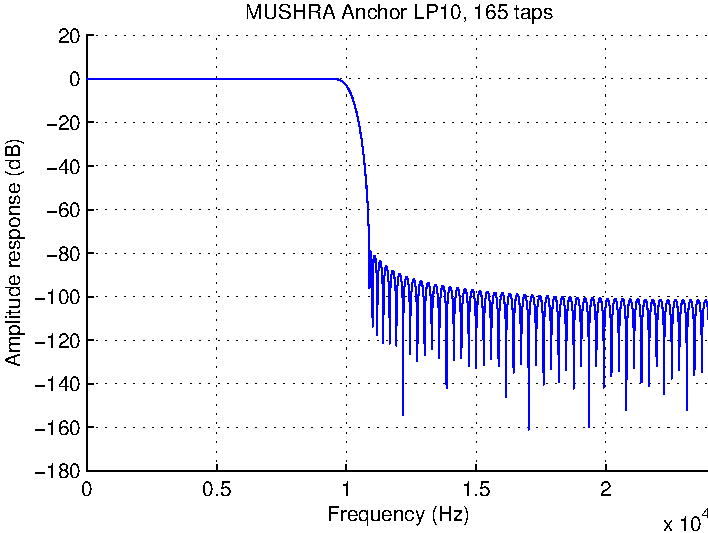
\includegraphics{LP10}
  \end{center}
  \caption{\SF Frequency response of the STL MUSHRA anchor LP10 -- Low-pass filter with cut-off frequency 10 kHz for a sampling frequency of 48 kHz (factor 1:1).
           \label{LP10-frq}
          }
\end{figure}
%------------- End of FIR filters response: frq for LP10 -------------


%--- Begin of FIR filters response: impulse response for LP10 --------
\begin{figure}[hbtp]
  \begin{center}
 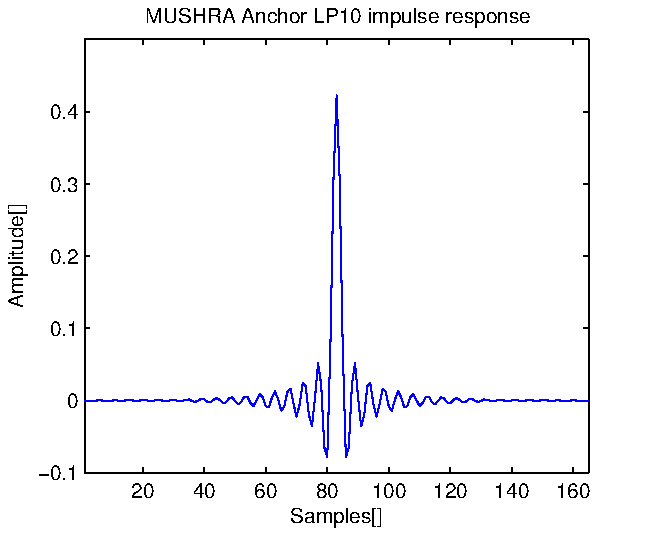
\includegraphics{LP10-h0}
  \end{center}
  \caption{\SF Impulse response of the STL MUSHRA anchor LP10 -- Low-pass filter with cut-off frequency 10 kHz for a sampling frequency of 48 kHz (factor 1:1).
           \label{LP10-ir}
          }
\end{figure}
%----- End of FIR filters response: impulse response for LP10 -----

%----------- Begin of FIR filters response: frq for LP12 filter  ----
\begin{figure}[hbtp]
  \begin{center}
% 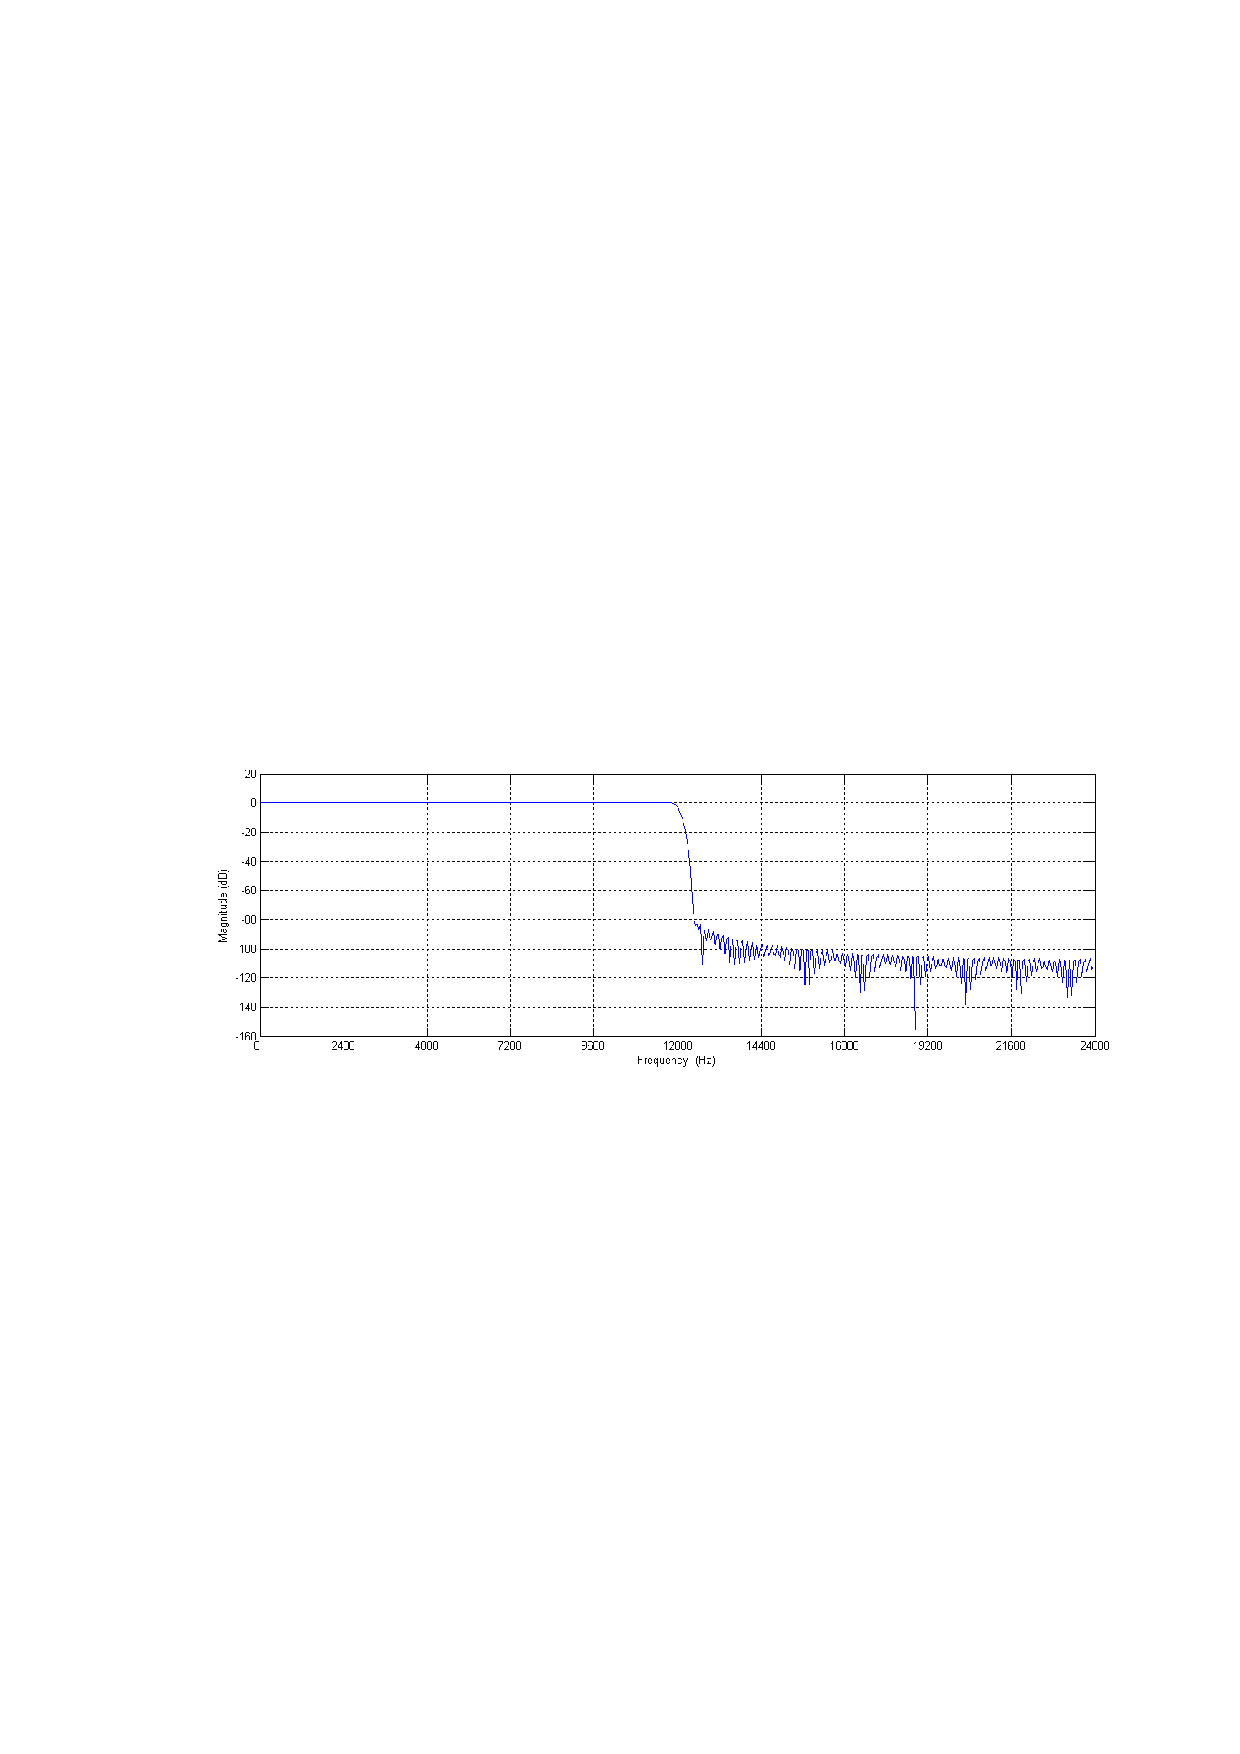
\includegraphics{LP12-h0}
 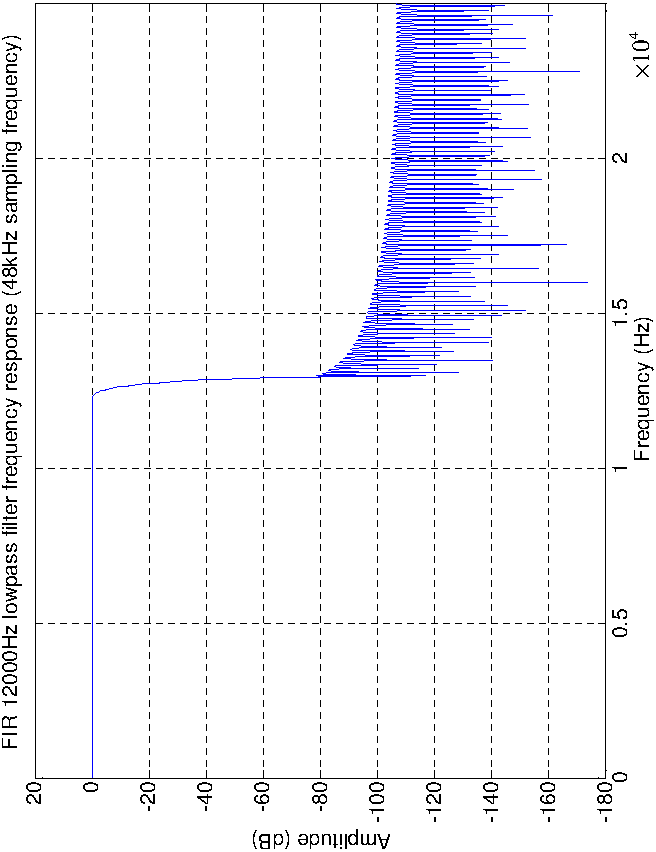
\includegraphics[angle=-90,scale=0.7]{LP12-h0new}
  \end{center}
  \caption{\SF Frequency response of the STL MUSHRA anchor LP12 -- Low-pass filter with cut-off frequency 12 kHz for a sampling frequency of 48 kHz (factor 1:1).
           \label{LP12-frq}
          }
\end{figure}
%------------- End of FIR filters response: frq for LP12 -------------


%--- Begin of FIR filters response: impulse response for LP12 --------
\begin{figure}[hbtp]
  \begin{center}
% 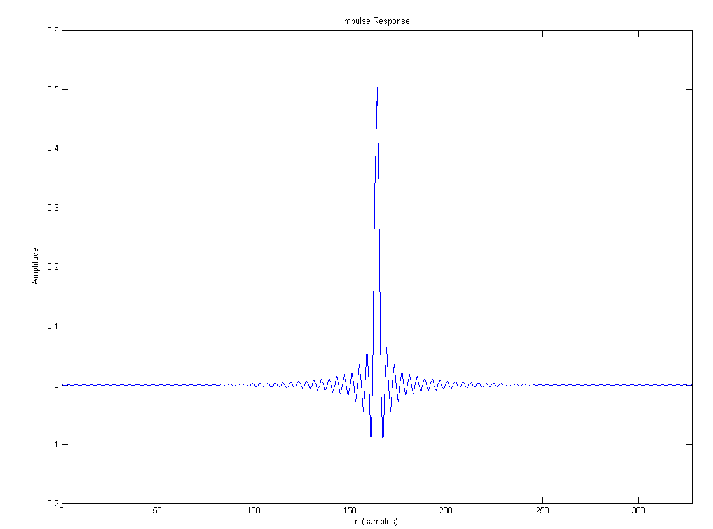
\includegraphics{LP12}
 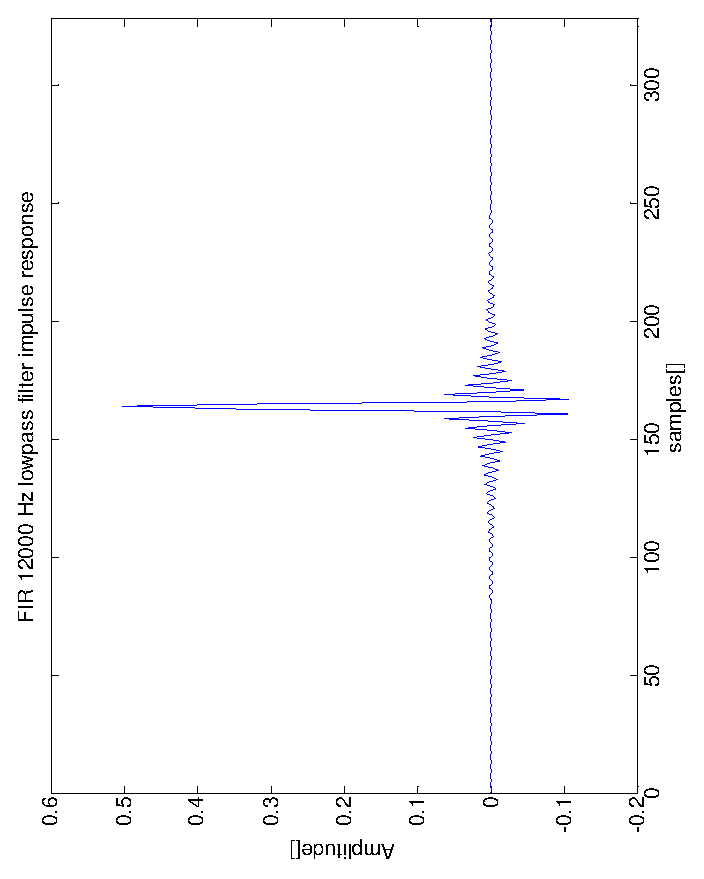
\includegraphics[angle=-90,scale=0.7]{LP12new}
  \end{center}
  \caption{\SF Impulse response of the STL MUSHRA anchor LP12 -- Low-pass filter with cut-off frequency 12 kHz for a sampling frequency of 48 kHz (factor 1:1).
           \label{LP12-ir}
          }
\end{figure}
%----- End of FIR filters response: impulse response for LP12 -----


%----------- Begin of FIR filters response: frq for LP14 filter  ----
\begin{figure}[hbtp]
  \begin{center}
 \includegraphics[scale=0.6]{LP14}
  \end{center}
  \caption{\SF Frequency response of the STL MUSHRA anchor LP14 -- Low-pass filter with cut-off frequency 14 kHz for a sampling frequency of 48 kHz (factor 1:1).
           \label{LP14-frq}
          }
\end{figure}
%------------- End of FIR filters response: frq for LP14 -------------

%--- Begin of FIR filters response: impulse response for LP14 --------
\begin{figure}[hbtp]
  \begin{center}
 \includegraphics[scale=0.6]{LP14-h0}
  \end{center}
  \caption{\SF Impulse response of the STL MUSHRA anchor LP14 -- Low-pass filter with cut-off frequency 14 kHz for a sampling frequency of 48 kHz (factor 1:1).
           \label{LP14-ir}
          }
\end{figure}
%----- End of FIR filters response: impulse response for LP14 -----

\flushfloats

%----------- Begin of FIR filters response: frq for LP20 filter  ----
\begin{figure}[hbtp]
  \begin{center}
 \includegraphics[scale=1.4]{LP20}
  \end{center}
  \caption{\SF Frequency response of the STL MUSHRA anchor LP20 -- Low-pass filter with cut-off frequency 20 kHz for a sampling frequency of 48 kHz (factor 1:1).
           \label{LP20-frq}
          }
\end{figure}
%------------- End of FIR filters response: frq for LP14 -------------

%--- Begin of FIR filters response: impulse response for LP20 --------
\begin{figure}[hbtp]
  \begin{center}
 \includegraphics[scale=1.4]{LP20-h0}
  \end{center}
  \caption{\SF Impulse response of the STL MUSHRA anchor LP20 -- Low-pass filter with cut-off frequency 20 kHz for a sampling frequency of 48 kHz (factor 1:1).
           \label{LP20-ir}
          }
\end{figure}
%----- End of FIR filters response: impulse response for LP20 -----
\flushfloats


%-.-.-.-.-.-.-.-.-.-.-.-.-.-.-.-.-
\mysubsubsection{{\tt *\_init} for the FIR module}

{\bf Syntax: }

{\tt
\#include "firflt.h"\\
SCD\_FIR *delta\_sm\_16khz\_init (void);\\
SCD\_FIR *hq\_down\_2\_to\_1\_init (void);\\
SCD\_FIR *hq\_up\_1\_to\_2\_init (void);\\
SCD\_FIR *hq\_down\_3\_to\_1\_init (void);\\
SCD\_FIR *hq\_up\_1\_to\_3\_init (void);\\
SCD\_FIR *irs\_8khz\_init (void);\\
SCD\_FIR *irs\_16khz\_init (void);\\
SCD\_FIR *linear\_phase\_pb\_2\_to\_1\_init (void);\\
SCD\_FIR *linear\_phase\_pb\_1\_to\_2\_init (void);\\
SCD\_FIR *linear\_phase\_pb\_1\_to\_1\_init (void);\\
SCD\_FIR *msin\_16khz\_init();\\
SCD\_FIR *mod\_irs\_16khz\_init (void);\\
SCD\_FIR *mod\_irs\_48khz\_init (void);\\
SCD\_FIR *rx\_mod\_irs\_8khz\_init(void);\\
SCD\_FIR *rx\_mod\_irs\_16khz\_init(void);\\
SCD\_FIR *psophometric\_8khz\_init (void);\\
SCD\_FIR *p341\_16k\_init (void);\\
SCD\_FIR *bp14k\_32khz\_init (void);\\
SCD\_FIR *bp5k\_16k\_init (void);\\
SCD\_FIR *bp100\_5k\_16khz\_init (void);\\
SCD\_FIR *bp20k\_48kHz\_init (void);\\
SCD\_FIR *LP1p5\_48kHz\_init (void);\\
SCD\_FIR *LP35\_48kHz\_init (void);\\
SCD\_FIR *LP7\_48kHz\_init (void);\\
SCD\_FIR *LP10\_48kHz\_init (void);\\
SCD\_FIR *LP12\_48kHz\_init (void);\\
SCD\_FIR *LP14\_48kHz\_init (void);\\
SCD\_FIR *L20\_48kHz\_init (void);\\
}


{\bf Prototypes: }   firflt.h

{\bf Description: }

{\tt delta\_sm\_16khz\_init} is the initialization routine for the
$\Delta_{SM}$ weighting filter for data sampled at 16 kHz using a
linear phase FIR filter structure. Input and output signals will be at
16 kHz. Code is in file {\tt fir-dsm.c} and its frequency response is
given in figure \ref{delta-sm-frq}.

{\tt hq\_up\_1\_to\_2\_init} is the initialization routine for high
quality FIR up-sampling filtering by a factor of 2. The -3 dB point
for this filter is located at approximately 3660 Hz. Code is in file
{\tt fir-flat.c} and its frequency and impulse response are given in
figures \ref{hq-frq-1-2}~(a) and \ref{ir-hq-up}~(top), respectively.

{\tt hq\_down\_2\_to\_1\_init} is the initialization routine for high
quality FIR down-sampling filtering by a factor of 2. The -3 dB point
for this filter is located at approximately 3660 Hz. Code is in file
{\tt fir-flat.c} and its frequency and impulse response are given in
figures \ref{hq-frq-1-2}~(b) and \ref{ir-hq-down}~(top), respectively.

{\tt hq\_up\_1\_to\_3\_init} is the initialization routine for high
quality FIR up-sampling filter by factor of 3. The -3 dB point for
this filter is located at approximately 3650 Hz. Code is in file {\tt
fir-flat.c} and its frequency and impulse response are given in
figures \ref{hq-frq-1-3}~(a) and \ref{ir-hq-up}~(bottom), respectively.

{\tt hq\_down\_3\_to\_1\_init} is the initialization routine for high
quality FIR down-sampling filtering by a factor of 3. The -3 dB point
for this filter is located at approximately 3650 Hz. Code is in file
{\tt fir-flat.c} and its frequency and impulse response are given in
figures \ref{hq-frq-1-3}~(b) and \ref{ir-hq-down}~(bottom),
respectively.

{\tt linear\_phase\_bp\_1\_to\_2\_init} is the initialization routine
for bandpass, FIR up-sampling filtering by a factor of 2. The -3 dB
points for this filter are located at approximately 98 and 3460
Hz. Code is in file {\tt fir-flat.c} and its frequency and impulse
response are given in figures \ref{hq-bandpass}~(b) and
\ref{ir-bandpass}~(b), respectively.

{\tt linear\_phase\_bp\_2\_to\_1\_init} is the initialization routine
for bandpass, FIR down-sampling filtering by a factor of 2. The -3 dB
points for this filter are located at approximately 98 and 3460
Hz. Code is in file {\tt fir-flat.c} and its frequency and impulse
response are given in figures \ref{hq-bandpass}~(a) and
\ref{ir-bandpass}~(a), respectively.

{\tt linear\_phase\_bp\_1\_to\_1\_init} is the initialization routine
for FIR 1:1 bandpass filtering. The -3 dB points for this filter are
located at approximately 98 and 3460 Hz. Code is in file {\tt
fir-flat.c} and its frequency and impulse response are given in
figures \ref{hq-bandpass}~(a) and \ref{ir-bandpass}~(a), respectively.

{\tt msin\_16khz\_init} is the initialization routine for the
high-pass, FIR 1:1 filter that simulates a mobile station input
characteristic. The -3 dB point for this filter is located at
approximately 195 Hz. Code is in file {\tt fir-flat.c} and its
frequency and impulse response are given in figures \ref{msin-frq} and
\ref{msin-ir}, respectively.

{\tt irs\_8khz\_init} is the initialization routine for the
transmit-side IRS weighting filter for data sampled at 8 kHz using a
linear phase FIR filter structure. Input and output signals will be at
8 kHz. Code is in file {\tt fir-irs.c} and its frequency and impulse
response are given in figures \ref{tx-reg-irs-frq}~(a) and
\ref{tx-reg-irs-ir}~(bottom), respectively.

{\tt irs\_16khz\_init} is the initialization routine for the
transmit-side IRS weighting filter for data sampled at 16 kHz using a
linear phase FIR filter structure. Input and output signals will be at
16 kHz. Code is in file {\tt fir-irs.c} and its frequency and impulse
response are given in figures \ref{tx-reg-irs-frq}~(b) and
\ref{tx-reg-irs-ir}~(top), respectively.

{\tt mod\_irs\_16khz\_init} is the initialization routine for the
transmit-side modified IRS weighting filter for data sampled at 16 kHz
using a linear phase FIR filter structure. Input and output signals
will be at 16 kHz since no rate change is performed by this function.
Code is in file {\tt fir-irs.c} and its frequency and impulse response
are given in figures \ref{tx-mod-irs-frq}~(a) and
\ref{tx-mod-irs-ir}~(a), respectively.

{\tt mod\_irs\_48khz\_init} is the initialization routine for the
transmit-side modified IRS weighting filter for data sampled at 48 kHz
using a linear phase FIR filter structure. Input and output signals
will be at 48 kHz since no rate change is performed by this function.
Code is in file {\tt fir-irs.c} and its frequency and impulse response
are given in figures \ref{tx-mod-irs-frq}~(b) and
\ref{tx-mod-irs-ir}~(b), respectively.

{\tt rx\_mod\_irs\_8khz\_init} is the initialization routine for the
receive-side modified IRS weighting filter for data sampled at 8 kHz
using a linear phase FIR filter structure. The -3 dB points for this
filter are located at approximately 285 Hz and 3610 Hz. Input and
output signals will be at 8 kHz since no rate change is performed by
this function. Code is in file {\tt fir-irs.c} and its frequency and
impulse response are given in figures \ref{rx-mod-irs-frq}~(a) and
\ref{rx-mod-irs-ir}~(a), respectively.

{\tt rx\_mod\_irs\_16khz\_init} is the initialization routine for the
receive-side modified IRS weighting filter for data sampled at 16 kHz
using a linear phase FIR filter structure. The -3 dB points for this
filter are located at approximately 285 Hz and 3610 Hz. Input and
output signals will be at 16 kHz since no rate change is performed by
this function. Code is in file {\tt fir-irs.c} and its frequency and
impulse response are given in figures \ref{rx-mod-irs-frq}~(b) and
\ref{rx-mod-irs-ir}~(b), respectively.

{\tt psophometric\_8khz\_init} is the initialization routine for the
O.41 psophometric weighting filter for data sampled at 8 kHz using a
linear phase FIR filter structure. Input and output signals will be at
8 kHz since no rate change is performed by this function. Code is in
file {\tt fir-pso.c} and its frequency response is given in figure
\ref{pso-08k-frq}.

{\tt p341\_16khz\_init} is the initialization routine for the P.341
send-side weighting filter for data sampled at 16 kHz. Input and
output signals will be at 16 kHz since no rate change is performed by
this function. Its frequency response is shown in figure
\ref{tx-p341-frq} and its impulse response is shown in figure
\ref{tx-p341-ir}. The -3 dB points for this filter are located at
approximately 50 and 7000 Hz. Code is in file {\tt fir-wb.c}.

{\tt bp14k\_32khz\_init} is the initialization routine for the
[50 Hz - 14 kHz] filter for data sampled at 32 kHz. Input and output
signals will be at 32 kHz since no rate change is performed by
this function. Its frequency response is shown in figure
\ref{50_14k-32k-frq} and its impulse response is shown in figure
\ref{50_14k-32k-ir}. The -3 dB points for this filter are located
at approximately 50 and 14000 Hz. Code is in file {\tt fir-wb.c}.

{\tt bp5k\_16khz\_init} is the initialization routine for a 
50 Hz - 5 kHz band limiting filter for wideband signals sampled at 16
kHz. Input and output signals will be at 16 kHz since no rate
change is performed by this function. Its frequency response is
shown in figure \ref{bp5k-16k-frq} and its impulse response is
shown in figure \ref{bp5k-16k-ir}. The -3 dB points for this
filter are located at approximately 50 and 4990 Hz. Code is in
file {\tt fir-wb.c}.

{\tt bp100\_5k\_16khz\_init} is the initialization routine for a
 100 Hz - 5 kHz band limiting filter for wideband signals sampled at 16
kHz. Input and output signals will be at 16 kHz since no rate
change is performed by this function. Its frequency response is
shown in figure \ref{bp100_5k-16k-frq} and its impulse response is
shown in figure \ref{bp100_5k-16k-ir}. The -3 dB points for this
filter are located at approximately 100 and 5000 Hz. Code is in
file {\tt fir-wb.c}.

{\tt bp20k\_48khz\_init} is the initialization routine for the
[20 Hz - 20 kHz] filter for data sampled at 48 kHz. Input and output
signals will be at 48 kHz since no rate change is performed by this
function. Its frequency response is shown in figure
\ref{bp20_20k-48k-frq} and its impulse response is shown in figure
\ref{bp20_20k-48k-ir}. The -3 dB points for this filter are located
at approximately 20 and 20000 Hz. Code is in file {\tt fir-wb.c}.

{\tt LP1p5\_48kHz\_init} is the initialization routine for a 1.5 kHz
low-pass filter for signals sampled at 48 kHz. Input and output
signals will be at 48 kHz since no rate change is performed by this
function. Its frequency response is shown in figure \ref{LP1p5-frq}
and its impulse response is shown in figure \ref{LP1p5-ir}. The -3
dB point for this filter is located at approximately 1500 Hz. Code
is in file {\tt fir-LP.c}.

{\tt LP35\_48kHz\_init} is the initialization routine for a 3.5 kHz
low-pass filter for signals sampled at 48 kHz. Input and output
signals will be at 48 kHz since no rate change is performed by this
function. Its frequency response is shown in figure \ref{LP35-frq}
and its impulse response is shown in figure \ref{LP35-ir}. The -3 dB
point for this filter is located at approximately 3500 Hz. Code is
in file {\tt fir-LP.c}.

{\tt LP7\_48kHz\_init} is the initialization routine for a 7 kHz
low-pass filter for signals sampled at 48 kHz. Input and output
signals will be at 48 kHz since no rate change is performed by this
function. Its frequency response is shown in figure \ref{LP7-frq}
and its impulse response is shown in figure \ref{LP7-ir}. The -3 dB
point for this filter is located at approximately 7000 Hz. Code is
in file {\tt fir-LP.c}.

{\tt LP10\_48kHz\_init} is the initialization routine for a 10 kHz
low-pass filter for signals sampled at 48 kHz. Input and output
signals will be at 48 kHz since no rate change is performed by this
function. Its frequency response is shown in figure \ref{LP10-frq}
and its impulse response is shown in figure \ref{LP10-ir}. The -3 dB
point for this filter is located at approximately 10000 Hz. Code is
in file {\tt fir-LP.c}.

{\tt LP12\_48kHz\_init} is the initialization routine for a 12 kHz
low-pass filter for signals sampled at 48 kHz. Input and output
signals will be at 48 kHz since no rate change is performed by this
function. Its frequency response is shown in figure \ref{LP12-frq}
and its impulse response is shown in figure \ref{LP12-ir}. The -3 dB
point for this filter is located at approximately 14000 Hz. Code is
in file {\tt fir-LP.c}.

{\tt LP14\_48kHz\_init} is the initialization routine for a 14 kHz
low-pass filter for signals sampled at 48 kHz. Input and output
signals will be at 48 kHz since no rate change is performed by this
function. Its frequency response is shown in figure \ref{LP14-frq}
and its impulse response is shown in figure \ref{LP14-ir}. The -3 dB
point for this filter is located at approximately 14000 Hz. Code is
in file {\tt fir-LP.c}.

{\tt LP20\_48kHz\_init} is the initialization routine for a 20 kHz
low-pass filter for signals sampled at 48 kHz. Input and output
signals will be at 48 kHz since no rate change is performed by this
function. Its frequency response is shown in figure \ref{LP20-frq}
and its impulse response is shown in figure \ref{LP20-ir}. The -3 dB
point for this filter is located at approximately 20000 Hz. Code is
in file {\tt fir-LP.c}.


\rulex{1mm}

{\bf Variables: }

None.

{\bf Return value: }

These functions return a pointer to a state variable structure of type
{\tt SCD\_FIR}.


%-.-.-.-.-.-.-.-.-.-.-.-.-.-.-.-.-.-
\mysubsubsection{\tt hq\_kernel}

{\bf Syntax: }

{\tt
\#include "firflt.h"\\
long hq\_kernel(long {\em lseg}, float {\em *x\_ptr},
              SCD\_FIR {\em *fir\_ptr},
              float {\em *y\_ptr});
}

{\bf Prototype: }    firflt.h

{\bf Source code: }  fir-lib.c

{\bf Description: }

This is the main entry routine for generic FIR filtering. It works as
a switch to specific up- and down-sampling FIR-kernel functions. The
adequate lower-lever filtering routine private to the filtering module
(which is not visible by the user) is defined by the initialization
routines. Currently, this function does not work properly for
sample-by-sample downsampling operation, i.e. when $lseg=1$. This
limitation should be corrected in a future version.

Please note that prior to the first call to {\tt hq\_kernel}, one of
the initialization routines {\tt hq\_*\_init} must be called
to allocate memory for state variables and the set the desired filter
coefficients.

After returning from this function, the state variables are saved to
allow segment-wise filtering through successive calls of {\tt
hq\_kernel}. This is useful when large files have to be processed.


{\bf Variables: }
\begin{Descr}{\DescrLen}
\item[\pbox{20mm}{\em lseg}] %\rulex{1mm}\\
        Number of input samples. Should be larger than 1 for proper
        downsampling operation.

\item[\pbox{20mm}{\em x\_ptr}] %\rulex{1mm}\\
        Array with input samples.

\item[\pbox{20mm}{\em fir\_ptr}] %\rulex{1mm}\\
        Pointer to FIR-struct.

\item[\pbox{20mm}{\em y\_ptr}] %\rulex{1mm}\\
        Pointer to output samples.
\end{Descr}

{\bf Return value: }

The number of filtered samples as a \long.



%-.-.-.-.-.-.-.-.-.-.-.-.-.-.-.-.-.-
\mysubsubsection{\tt hq\_reset}

{\bf Syntax: }

{\tt
\#include "firflt.h"\\
void hq\_reset (SCD\_FIR {\em *fir\_ptr});
}

{\bf Prototype: }    firflt.h

{\bf Source code: }  fir-lib.c

{\bf Description: }

Clear state variables in {\tt SCD\_FIR} struct; deallocation of filter
structure memory is not done. Please note that {\em fir\_ptr} should
point to a valid {\tt SCD\_FIR} structure, which was allocated by an
earlier call to one of the FIR initialization routines {\tt
hq\_*\_init}.

{\bf Variables: }
\begin{Descr}{\DescrLen}
\item[\pbox{20mm}{\em fir\_ptr}] %\rulex{1mm}\\
        Pointer to a valid structure {\tt SCD\_FIR}.
\end{Descr}


{\bf Return value: }

        None.



%-.-.-.-.-.-.-.-.-.-.-.-.-.-.-.-.-.-
\mysubsubsection{\tt hq\_free}

{\bf Syntax: }

{\tt
\#include "firflt.h"\\
void hq\_free (SCD\_FIR {\em *fir\_ptr});
}

{\bf Prototype: }    firflt.h

{\bf Source code: }  fir-lib.c

{\bf Description: }

Deallocate memory, which was allocated by an earlier call to one of the
FIR initialization routines {\tt hq\_*\_init}. Note that the pointer to
the structure {\tt SCD\_FIR} must not be a null pointer.

{\bf Variables: }
\begin{Descr}{\DescrLen}
\item[\pbox{20mm}{\em fir\_ptr}] Pointer to a structure of type {\tt SCD\_FIR}.
\end{Descr}

{\bf Return value: }

None.


%-.-.-.-.-.-.-.-.-.-.-.-.-.-.-.-.-
\subsection{IIR Module}

The IIR module contains filters whose main use is for asynchronous
filtering. For telephony bandwidth asynchronous filtering, PCM filters
are available in both cascade and parallel IIR filter forms. For
wideband speech (50--7000 Hz), 3:1 and 1:3 rate-change factor filters
are available. A transmit-side IRS filter for speech sampled at 8 kHz
is also available in this module as an example of implementation of an
IIR cascade-form filter.

The PCM filters have been designed for {\em sampling rates} of 8 and 16
kHz. It should be noted that the G.712 mask is specified in terms of Hz,
rather than normalized frequencies. Therefore this applies only to rate
conversions of factor 2, i.e., 8 kHz to 16 kHz and 16 kHz to 8 kHz.
The frequency responses of the implemented PCM filters are shown in
figure \ref{pcm-frq}.

Since the digital filters need memory, state variables are needed. In
the STL, a type {\tt SCD\_IIR} has been defined for parallel-form IIR
filters, containing the past memory samples as well as filter
coefficients and other control variables. Its fields are as follows:

\rulex{10mm} \begin{minipage}{130mm} \normalsize
 {\em nblocks}  \dotfill \parbox{100mm}{\SF Number of coefficient sets}\\
 {\em idown}    \dotfill \parbox{100mm}{\SF Up-/down-sampling factor}\\
 {\em k0}       \dotfill \parbox{100mm}{\SF Start index in next segment}\\
 {\em gain}     \dotfill \parbox{100mm}{\SF Gain factor}\\
 {\em direct\_cof} \dotfill \parbox{100mm}{\SF Direct path coefficient}\\
 {\em b[3]}     \dotfill \parbox{100mm}{\SF Pointer to numerator coefficients}\\
 {\em c[2]}     \dotfill \parbox{100mm}{\SF Pointer to denominator coefficients}\\
 {\em T[2]}     \dotfill \parbox{100mm}{\SF Pointer to state variables}\\
 {\em hswitch}  \dotfill \parbox{100mm}{\SF Switch to IIR-kernel: Up or
                                          down-sampling}\\
\end{minipage}

For the cascade-form IIR filters, the state variable structure defined
is {\tt CASCADE\_IIR} which is slightly different from the one for the
parallel form structure:

\rulex{10mm} \begin{minipage}{130mm} \normalsize
  {\em nblocks}  \dotfill \parbox{100mm}{\SF Number of stages in cascade}\\
  {\em idown}    \dotfill \parbox{100mm}{\SF Up-/down-sampling factor}\\
  {\em k0}       \dotfill \parbox{100mm}{\SF Start index in next segment}\\
  {\em gain}     \dotfill \parbox{100mm}{\SF Gain Factor}\\
  {\em a[2]}     \dotfill \parbox{100mm}{\SF Pointer to numerator coefficients}\\
  {\em b[2]}     \dotfill \parbox{100mm}{\SF Pointer to denominator coefficients}\\
  {\em T[4]}     \dotfill \parbox{100mm}{\SF Pointer to state variables}\\
  {\em hswitch}  \dotfill \parbox{100mm}{\SF Switch to IIR-kernel: Up or
                                          down-sampling}\\
\end{minipage}

It should be noted that the values of the fields must not be altered,
and for most purposes they are not needed by the user.  The relevant
routines for each module are described in the next sections.

%--------------- Cascade G.712 @ 8 kHz frequency response ---------------------
%Box dimension: 15.24cm x  8.89cm
\begin{figure}[hbtp]
  \begin{center}
\includegraphics{pcm_1_1}
    \\
  \end{center}
  \caption{\SF Frequency response of the cascade implementation of the G.712
               standard PCM filter for data sampled at 8 kHz.
               \label{casc-g712-8k}}
\end{figure}
%----------------------------------------------------------------------------


%--------------- IIR TX IRS @ 8 kHz ----------------------------
%Box dimension: 15.24cm x  8.89cm
\begin{figure}[tp]
  \begin{center}
\includegraphics{casc-irs}
    \\
  \end{center}
  \caption{ Frequency response of an IIR cascade implementation of
            the P.48 ``full'' transmit-side IRS weighting filter for
            data sampled at 8 kHz.
            \label{casc-irs-8k} }
\end{figure}
%---------------------------------------------------------------------------


%--------------  Async 1:3, 3:1 IIR filter frequency response ----------------
\begin{figure}[hbtp]
  \begin{center}
\includegraphics{asy1_3}
    \\
   (a) Flat low-pass up-sampling by a factor of 1:3.

\includegraphics{asy3_1}
    \\
   (b) Flat low-pass down-sampling by a factor of 3:1.

  \end{center}
  \caption{\SF Flat low-pass IIR filter frequency response
               with factors 1:3 and 3:1 for sampling rates of 16000
               and 48000 Hz.\label{casc-lp-3-1}}
\end{figure}
%----------------------------------------------------------------------------


%--------------- Async IIR 3:1, 1:3 filter impulse response ------------------
%Box dimension (for a. and b.): 15.24cm x  8.89cm
\begin{figure}[tp]
  \begin{center}
\includegraphics{asynuph0}
    \\
   (a) 1:3 up-sampling factor

\includegraphics{asyndwh0}
    \\
   (b) 3:1 down-sampling factor
  \end{center}
  \caption{ Impulse response for 1:3 and 3:1 cascade-form low-pass IIR filter.
            \label{ir-casc-lp-3-1}}
\end{figure}
%---------------------------------------------------------------------------


%--------------- Std.PCM IIR filter frequency response ---------------------
\begin{figure}[hbtp]
  \begin{center}
\includegraphics{pcm_1_2}
    \\
   (a) G.712 for input samples at 8 kHz, up-sampling factor 1:2

\includegraphics{pcm_2_1}
    \\
   (b) G.712 for input samples at 16 kHz, down-sampling factor 2:1 or 1:1

  \end{center}
  \caption{\SF Standard PCM (G.712) quality filter response.\label{pcm-frq}}
\end{figure}
%----------------------------------------------------------------------------


%--------------- Std.PCM filter impulse response ----------------------------
%Box dimension: 16.05cm x 18.03cm
\begin{figure}[tp]
  \begin{center}
\includegraphics{pcm-h0}
  \end{center}
  \caption{ \SF Impulse response for G.712 filters (Top: factor 1:1;
                Middle: factor 1:2; Bottom: factor 2:1).
                \label{pcm-ir}}
\end{figure}
%------------------ End of IIR filter freq. response ---------------------


%-.-.-.-.-.-.-.-.-.-.-.-.-.-.-.-.-.-
\mysubsubsection{\tt iir\_*\_init}

{\bf Syntax: }

% NOTE: the G in iir_G712_8khz_init() is INDEED upper case!!!
{\tt
\#include "iirflt.h"\\
CASCADE\_IIR *iir\_G712\_8khz\_init (void);\\
CASCADE\_IIR *iir\_irs\_8khz\_init (void);\\
CASCADE\_IIR *iir\_casc\_lp\_3\_to\_1\_init(void);\\
CASCADE\_IIR *iir\_casc\_lp\_1\_to\_3\_init(void);\\
}

{\bf Prototypes: }   iirflt.h

{\bf Description: }

{\tt iir\_G712\_8khz\_init} initializes an 8 kHz cascade IIR filter
structure for a standard PCM (G.712) filtering. Input and output
signals will be at 8 kHz since no rate change is performed by this
function. The -3 dB points for this filter are located at
approximately 230 and 3530 Hz.  Its source code is found in file {\tt
cascg712.c} and its frequency response is given in figure
\ref{casc-g712-8k}.

{\tt iir\_irs\_8khz\_init} initializes an 8 kHz cascade IIR filter
structure for a transmit-side P.48 IRS non-linear phase
filtering. Input and output signals will be at 8 kHz since no rate
change is performed by this function. Its source code is found in file
{\tt iir-irs.c} and its frequency response is given in figure
\ref{casc-irs-8k}.

{\tt iir\_casc\_lp\_3\_to\_1\_init} is the initialization routine for
IIR low-pass filtering with a down-sampling factor of 3:1. Although
this filter is relatively independent of the sampling
rate,\footnote{\SF Since this is a low-pass filter, change of sampling
rate implies in change of the lower and upper cutoff frequencies.} it
was originally designed for asynchronization filtering of 16 kHz
sampled speech. The -3 dB point for this filter is located at
approximately 7055 Hz. Its source code is found in file {\tt
iir-flat.c} and its frequency and impulse response are given in figures
\ref{casc-lp-3-1}~(a) and \ref{ir-casc-lp-3-1}~(a), respectively.

{\tt iir\_casc\_lp\_1\_to\_3\_init} is the initialization routine for
IIR low-pass filtering with a up-sampling factor of 1:3. Although this
filter is relatively independent of the sampling rate, it was
originally designed for asynchronization filtering of 16 kHz sampled
speech. The -3 dB point for this filter is located at approximately
7055 Hz. Its source code is found in file {\tt iir-flat.c} and its
frequency and impulse response are given in figures
\ref{casc-lp-3-1}~(b) and \ref{ir-casc-lp-3-1}~(b), respectively.


\newpage

%-.-.-.-.-.-.-.-.-.-.-.-.-.-.-.-.-.-
\mysubsubsection{\tt cascade\_iir\_kernel}

{\bf Syntax: }

{\tt
\#include "iirflt.h"\\
long cascade\_iir\_kernel (\ttpbox{110mm}{
             long {\em lseg}, float {\em *x\_ptr}, CASCADE\_IIR
                 {\em *iir\_ptr}, \\ float {\em *y\_ptr});
         }
}

{\bf Prototype: }    iirflt.h

{\bf Source code: }  iir-lib.c

{\bf Description: }

General function for implementing filtering using a cascade-form IIR
filter previously initialized by one of the {\tt iir\_*\_init()} routines.

{\bf Variables: }
\begin{Descr}{\DescrLen}
\item[\pbox{20mm}{\em lseg}] %\rulex{1mm}\\
        Number of input samples.

\item[\pbox{20mm}{\em x\_ptr}] %\rulex{1mm}\\
        Array with input samples.

\item[\pbox{20mm}{\em iir\_ptr}] %\rulex{1mm}\\
        Pointer to a cascade-form IIR-struct {\tt CASCADE\_IIR}.

\item[\pbox{20mm}{\em y\_ptr}] %\rulex{1mm}\\
        Pointer to output samples.
\end{Descr}


{\bf Return value: }

The number of output samples is returned as a long.

%-.-.-.-.-.-.-.-.-.-.-.-.-.-.-.-.-.-
\mysubsubsection{\tt cascade\_iir\_reset}

{\bf Syntax: }

{\tt
\#include "iirflt.h"\\
void cascade\_iir\_reset (\ttpbox{110mm}{
             CASCADE\_IIR {\em *iir\_ptr});
         }
}

{\bf Prototype: }    iirflt.h

{\bf Source code: }  iir-lib.c

{\bf Description: }

Clear state variables in {\tt CASCADE\_IIR} structure, which have been
initialized by a previous call to one of the initialization
functions. Memory previously allocated is not released.

{\bf Variables: }
\begin{Descr}{\DescrLen}
\item[\pbox{20mm}{\em iir\_ptr}] %\rulex{1mm}\\
        Pointer to struct {\tt CASCADE\_IIR}, previously initialized
        by a call to one of the initialization routines.
\end{Descr}

{\bf Return value: }

None.

\newpage

%-.-.-.-.-.-.-.-.-.-.-.-.-.-.-.-.-.-
\mysubsubsection{\tt cascade\_iir\_free}

{\bf Syntax: }

{\tt
\#include "iirflt.h"\\
void cascade\_iir\_free (\ttpbox{110mm}{
             SCD\_IIR {\em *iir\_ptr});
         }
}

{\bf Prototype: }    iirflt.h

{\bf Source code: }  iir-lib.c

{\bf Description: }

Deallocate memory, which was allocated by an earlier call to one of
the cascade-form IIR filter initialization routines described before.
{\tt iir\_prt} must not be a NULL pointer.

{\bf Variables: }
\begin{Descr}{\DescrLen}
\item[\pbox{20mm}{\em iir\_ptr}] %\rulex{1mm}\\
        Pointer to struct {\tt CASCADE\_IIR}, previously initialized
        by a call to one of the initialization routines.
\end{Descr}


{\bf Return value: }

None.


%-.-.-.-.-.-.-.-.-.-.-.-.-.-.-.-.-.-
\mysubsubsection{\tt stdpcm\_*\_init}

{\bf Syntax: }

{\tt
\#include "iirflt.h"\\
SCD\_IIR *stdpcm\_16khz\_init (void);\\
SCD\_IIR *stdpcm\_1\_to\_2\_init (void);\\
SCD\_IIR *stdpcm\_2\_to\_1\_init (void);
}

{\bf Prototypes: }   iirflt.h

{\bf Description: }

{\tt stdpcm\_16khz\_init} initializes a 16 kHz IIR filter structure
for standard PCM (G712) filtering. Input and output signals will be at
16 kHz since no rate change is performed by this function. The -3 dB
points for this filter are located at approximately 174 and 3630 Hz.
Source code is found in file {\tt iir-g712.c} and its frequency and
impulse response are given in figures \ref{pcm-frq}(b) and
\ref{pcm-ir} (top), respectively.

{\tt stdpcm\_1\_to\_2\_init} initializes standard PCM filter
coefficients for filtering by the generic filtering routine {\tt
stdpcm\_kernel}, for input signals at 8 kHz, generating the output at
16 kHz. The -3 dB points for this filter are located at approximately
174 and 3630 Hz. Source code is found in file {\tt iir-g712.c} and its
frequency and impulse response are given in figures \ref{pcm-frq}(a)
and \ref{pcm-ir} (middle), respectively.

{\tt stdpcm\_2\_to\_1\_init} initializes standard PCM filter
coefficients for filtering by the generic filtering routine {\tt
stdpcm\_kernel} for input signals at 16 kHz, generating the output at
8 kHz. The -3 dB points for this filter are located at approximately
174 and 3630 Hz. Source code is found in file {\tt iir-g712.c} and its
frequency and impulse response are given in figures \ref{pcm-frq}(b)
and \ref{pcm-ir} (bottom), respectively.

{\bf Variables: }

None.

{\bf Return value: }

This function returns a pointer to a state variable structure of type
{\tt SCD\_IIR}.



%-.-.-.-.-.-.-.-.-.-.-.-.-.-.-.-.-.-
\mysubsubsection{\tt stdpcm\_kernel}

{\bf Syntax: }

{\tt
\#include "iirflt.h"\\
long stdpcm\_kernel (\ttpbox{110mm}{
             long {\em lseg}, float {\em *x\_ptr}, SCD\_IIR
                 {\em *iir\_ptr}, \\ float {\em *y\_ptr});
         }
}

{\bf Prototype: }    iirflt.h

{\bf Source code: }  iir-lib.c

{\bf Description: }

General function to perform filtering using a parallel-form
IIR  filter previously initialized by one of the appropriate parallel-form
{\tt *\_init()} routines available.

{\bf Variables: }
\begin{Descr}{\DescrLen}
\item[\pbox{20mm}{\em lseg}] %\rulex{1mm}\\
        Number of input samples.

\item[\pbox{20mm}{\em x\_ptr}] %\rulex{1mm}\\
        Array with input samples.

\item[\pbox{20mm}{\em iir\_ptr}] %\rulex{1mm}\\
        Pointer to a parallel-form IIR-struct {\tt SCD\_IIR}.

\item[\pbox{20mm}{\em y\_ptr}] %\rulex{1mm}\\
        Pointer to output samples.
\end{Descr}


{\bf Return value: }

This function returns the number of output samples as a \long.


%-.-.-.-.-.-.-.-.-.-.-.-.-.-.-.-.-.-
\mysubsubsection{\tt stdpcm\_reset}

{\bf Syntax: }

{\tt
\#include "iirflt.h"\\
void stdpcm\_reset (\ttpbox{110mm}{
             SCD\_IIR {\em *iir\_ptr});
         }
}

{\bf Prototype: }    iirflt.h

{\bf Source code: }  iir-lib.c

{\bf Description: }

Clear state variables in {\tt SCD\_IIR} structure, which have been
initialized by a previous call to one of the init functions. Memory
previously allocated is not released.

{\bf Variables: }
\begin{Descr}{\DescrLen}
\item[\pbox{20mm}{\em iir\_ptr}] %\rulex{1mm}\\
        Pointer to struct {\tt SCD\_IIR}, previously initialized by a call to
        one of the initialization routines.
\end{Descr}

{\bf Return value: }

None.


%-.-.-.-.-.-.-.-.-.-.-.-.-.-.-.-.-.-
\mysubsubsection{\tt stdpcm\_free}

{\bf Syntax: }

{\tt
\#include "iirflt.h"\\
void stdpcm\_free (\ttpbox{110mm}{
             SCD\_IIR {\em *iir\_ptr});
         }
}

{\bf Prototype: }    iirflt.h

{\bf Source code: }  iir-lib.c

{\bf Description: }

Release memory which was allocated by an earlier call to one of
the parallel-form IIR filter initialization routines described before.
The parameter {\tt iir\_prt} must not be a null pointer.

{\bf Variables: }
\begin{Descr}{\DescrLen}
\item[\pbox{20mm}{\em iir\_ptr}] %\rulex{1mm}\\
        Pointer to struct {\tt SCD\_IIR}, previously initialized by a call to
        one of the initialization routines.
\end{Descr}


{\bf Return value: }

None.


%..................................
\section {Tests and portability} \label{RATE-Tests}

Compliance with the \ROs~ was verified by checking the frequency
response of the filters and the size of the output files. Frequency
response was obtained by feeding the filtering routines with sinewaves
and calculating the ratio in dB, for each frequency of interest.

Portability of this module was checked by running the same speech file
on a proven platform and on a test platform. Comparison of both
processed files should show either no differences or yield equivalent
results.\footnote{\SF Some differences may appear in the output files,
but for a few samples and by no more than 1 LSB. As an example, in the
tests for checking VAX and SUN-OS, one of the files differed in 3
samples out of 49152 for a cascade of high-quality up- and
down-sampling of 1:6 and 6:1. For small rate change factors,
differences are unlikely.} Tests were performed in the VAX/VMS
environment with VAX-C and gcc, in MSDOS with Borland Turbo C++
Version 1.00 and gcc (DJGPP), in SunOS with cc, acc, and gcc, and in
HPUX with gcc.


%..................................
\section {Examples} \label{Rate-exp}


%..........................................................................
\subsection {Description of the demonstration programs}

Three programs are provided as demonstration programs for the RATE module,
firdemo.c, iirdemo.c, and filter.c.

Programs {\tt firdemo.c} and {\tt iirdemo.c} were the first demonstration
programs for the rate change module. The former is found in directory
{\tt fir} of the STL and contains a cascade processing of the FIR
filters available upto the STL96. The latter is found in directory
{\tt iir} of the STL and contains a cascade processing of the IIR
filters available up to the STL96. However, because of the increasing
static memory requirement for cascade processing that came with the
introduction of new filters in the STL, these two programs became
prohibitive and their maintenance was discontinued. They are still
functional, although outdated.

Program {\tt filter.c} is a single demonstration program that incorporates both
IIR and FIR filters in the STL and has been kept up-to-date as new
filters are added to the STL. Compared to the firdemo.c and iirdemo.c
programs, filter.c can only perform one filtering operation per
pass, while firdemo.c and iirdemo.c could perform a number of 1:1
operations combined with two up-sampling and two downsampling
operations. Hence, several calls of the filter program are necessary
to implement what was accomplished by a single call of firdemo.c and
iirdemo.c, in addition to the cumulative quantization noise (from the
successive float-to-short conversions). In applications where multiple
filtering is needed and the user is concerned with the quantization
noise accumulation, a custom-made program could be used e.g. based on
a specialization of either firdemo.c, iirdemo.c, or filter.c.

%..........................................................................
\subsection {Example: Calculating frequency responses}

The following C code exemplifies the use of some of the filter
functions available in the STL. The C code generates a number of tones
which are specified by the user (lower, upper, and step frequencies).
The frequency response is obtained by calculating the power change for
each single frequency before and after filtered by the selected
filter.

{\tt\small
\begin{verbatim}
#include <stdio.h>
#include <stdlib.h>
#include <math.h>

/* UGST MODULES */
#include "ugstdemo.h"
#include "iirflt.h"
#include "firflt.h"

/* Other stuff */
#define TWO_PI (8*atan(1.0))
#define QUIT(m,code) {fprintf(stderr,m); exit((int)code);}

void main(argc, argv)
  int             argc;
  char           *argv[];
{
  SCD_FIR        *fir_state;
  SCD_IIR        *iir_state;
  float          *BufInp, *BufOut;
  char            F_type[20];
  long            j, N, N2;
  long            inp_size, out_size;
  double          f, f0, fstep, ff, fs, inp_pwr, H_k;
  char            is_fir;

  /* Preamble */
  N = 256; N2 = 20; inp_size = N * N2;

  /* Read parameters for processing */
  GET_PAR_S(1, "_Filter type(irs,hq2,hq3,pcm,pcm1): ... ", F_type);
  GET_PAR_D(2, "_Start frequency [Hz]: ................ ", f0);
  GET_PAR_D(3, "_Stop frequency [Hz]: ................. ", ff);
  GET_PAR_D(4, "_Frequency step [Hz]: ................. ", fstep);
  FIND_PAR_D(5, "_Sampling Frequency [Hz]: ............. ", fs, 8000);

  /* Check consistency of upper and lower frequencies */
  ff = (ff >= fs / 2)? (fs / 2) : ff;
  if (f0 < 2.0 / (double) inp_size * fs && f0 != 0.0)
    f0 = 2.0 / (double) inp_size *fs;

  /* Normalization of frequencies */
  f0 /= fs; ff /= fs; fstep /= fs;

  /* Set flag to filter type: IIR or FIR */
  is_fir = (strncmp(F_type,"pcm",3)==0 || strncmp(F_type,"PCM",3)==0)
           ? 0 : 1;

  /* ... CHOOSE CORRECT FILTER INITIALIZATION ... */
  /*
   * Filter type: irs - IRS weighting 2:1 or 1:2 factor:
   *                     . fs ==  8000 -> up-sample: 1:2
   *                     . fs == 16000 -> down-sample: 2:1
  */
  if (strncmp(F_type, "irs", 3) == 0 || strncmp(F_type, "IRS", 3) == 0)
  {
    if (fs == 8000)
      fir_state = irs_8khz_init();
    else if (fs == 16000)
      fir_state = irs_16khz_init();
    else
      QUIT("IRS Implemented only for 8 and 16 kHz\n", 15);
  }
  /*
   * Filter type: hq2 - High-quality 2:1 or 1:2 factor:
   *                    . fs ==  8000 -> up-sample: 1:2
   *                    . fs == 16000 -> down-sample: 2:1
   *              hq3 - High-quality 3:1 or 3:1 factor
   *                    . fs ==  8000 -> up-sample: 1:3
   *                    . fs == 16000 -> down-sample: 3:1
  */
  else if (strncmp(F_type,"hq",2)==0 || strncmp(F_type,"HQ",2)==0)
  {
    if (fs == 8000)             /* It is up-sampling! */
      fir_state = F_type[2] == '2'
        ? fir_up_1_to_2_init()
        : fir_up_1_to_3_init();
    else                        /* It is down-sampling! */
      fir_state = F_type[2] == '2'
        ? fir_down_2_to_1_init()
        : fir_down_3_to_1_init();
  }
  /*
   * Filter type: pcm  - Standard PCM quality 2:1 or 1:2 factor:
   *                    . fs ==  8000 -> up-sample: 1:2
   *                    . fs == 16000 -> down-sample: 2:1
   *              pcm1 - Standard PCM quality with 1:1 factor
   *                    . fs ==  8000 -> unimplemented
   *                    . fs == 16000 -> OK, 1:1 at 16 kHz
  */
  else if (strncmp(F_type,"pcm",3)==0 || strncmp(F_type,"PCM",3)==0)
  {
    if (strncmp(F_type,"pcm1", 4)==0 || strncmp(F_type,"PCM1",4)==0)
    {
      if (fs == 16000)
        iir_state = stdpcm_16khz_init();
      else
        QUIT("Unimplemented: PCM w/ factor 1:1 for given fs\n", 10);
    }
    else
      iir_state = (fs == 8000)
        ? stdpcm_1_to_2_init()  /* It is up-sampling! */
        : stdpcm_2_to_1_init(); /* It is down-sampling! */
  }

  /* Calculate Output buffer size */
  if (is_fir)
    out_size = (fir_state->hswitch=='U')
               ? inp_size * fir_state->dwn_up
               : inp_size / fir_state->dwn_up;
  else
    out_size = (iir_state->hswitch=='U')
               ? inp_size * iir_state->idown
               : inp_size / iir_state->idown;

  /* Allocate memory for input buffer */
  if ((BufInp = (float *) calloc(inp_size, sizeof(float))) == NULL)
    QUIT("Can't allocate memory for data buffer\n", 10);

  /* Allocate memory for output buffer */
  if ((BufOut = (float *) calloc(out_size, sizeof(float))) == NULL)
    QUIT("Can't allocate memory for data buffer\n", 10);

  /* Filtering operation */
  for (f = f0; f <= ff; f += fstep)
  {
    /* Reset memory */
    memset(BufOut, '\0', out_size * sizeof(float));

    /* Adjust top (NORMALIZED!) frequency, if needed */
    if (fabs(f - 0.5) < 1e-8/fs) f -= (0.05*fstep);

    /* Calculate as a temporary the frequency in radians */
    inp_pwr = f * TWO_PI;

    /* Generate sine samples with peak 20000 ... */
    for (j = 0; j < inp_size; j++)
      BufInp[j] = 20000.0 * sin(inp_pwr * j);

    /* Calculate power of input signal */
    for (inp_pwr = 0, j = 0; j < inp_size; j++)
      inp_pwr += BufInp[j] * BufInp[j];

    /* Convert to dB */
    inp_pwr = 10.0 * log10(inp_pwr / (double) inp_size);

    /* Filtering the whole buffer ... */
    j = (is_fir)
        ? fir_kernel(inp_size, BufInp, fir_state, BufOut)
        : stdpcm_kernel(inp_size, BufInp, iir_state, BufOut);

    /* Compute power of output signal; discard initial 2*N samples */
    for (H_k = 0, j = 2 * N; j < out_size - 2 * N; j++)
      H_k += BufOut[j] * BufOut[j];

    /* Convert to dB */
    H_k = 10 * log10(H_k / (double) (out_size - 4 * N)) - inp_pwr;

    /* Printout of gain at the current frequency */
    printf("\nH( %4.0f ) \t = %7.3f dB\n", f * fs, H_k);
  }
}
\end{verbatim}
}
